\chapter{The Kendall and Mallows Kernels for Permutations}
\label{chap:kendall}

\begin{chapabstract}

\textrm{{\bf Abstract:}} We show that the widely used Kendall tau correlation coefficient and the related Mallows kernel are positive definite kernels for permutations. They offer computationally attractive alternatives to more complex kernels on the symmetric group to learn from rankings, or learn to rank. We show how to extend these kernels to partial rankings, multivariate rankings and uncertain rankings. Examples are presented on how to formulate typical problems of learning from rankings such that they can be solved with state-of-the-art kernel algorithms. We demonstrate promising results on clustering heterogeneous rank data and high-dimensional classification problems in biomedical applications. This study has been published as joint work with Jean-Philippe Vert \cite{Jiao2015Kendall, Jiao2017Kendall}.
\linebreak
\vskip 0.1in
\noindent \textrm{{\bf R�sum�:}}

\end{chapabstract}

\section{Introduction}
\label{sec2:introduction}

A permutation is a 1-to-1 mapping from a finite set into itself. Assuming the finite set is ordered, a permutation can equivalently be represented by a total ranking of the elements of the set. Permutations are ubiquitous in many applications involving preferences, rankings or matching, such as modeling and analyzing data describing the preferences or votes of a population \cite{Diaconis1988Group, Marden1996Analyzing}, learning or tracking correspondences between sets of objects \cite{Huang2009Fourier}, or estimating a consensus ranking that best represents a collection of individual rankings \cite{Dwork2001Rank,Ailon2008Aggregating,Arrow2012Social}. Another potentially rich source of rank data comes from real-valued vectors in which the relative ordering of the values of multiple features is more important than their absolute magnitude. For example, in the case of high-dimensional gene expression data, \cite{Geman2004Classifying} showed that simple classifiers based on binary comparisons between the expression of different genes in a sample show competitive prediction accuracy with much more complex classifiers built on quantitative gene expression levels, a line of thoughts that have been further investigated by \cite{Tan2005Simple, Xu2005Robust, Lin2009ordering}. In these approaches, an $n$-dimensional feature vector is first transformed into a vector of ranks by sorting its entries, which are presented as input to training a classifier. 

Working with permutations is, however, computationally challenging. There are $n!$ permutations over $n$ items, suggesting that various simplifications or approximations are necessary in pursuit of efficient algorithms to analyze or learn permutations. Such simplifications include for example, reducing ranks to a series of binary decisions \cite{Ailon2008Aggregating, Balcan2008Robust}, or estimating a parametric distribution over permutations \cite{Lebanon2008Non, Helmbold2009Learning, Huang2009Fourier}. 


Kernel algorithms form a class of methods that have been proved successful in numerous applications and enjoy great popularity in the machine learning community \cite{Cortes1995Support,Vapnik1998Statistical,Schoelkopf2002Learning,Shawe-Taylor2004Kernel}. The essential idea behind these methods is to define a symmetric positive definite kernel $K:\mathcal{X}\times \mathcal{X} \to \mathbb{R}$ over an input space $\mathcal{X}$, which expresses our belief of similarities between pairs of points in the input space, and which implicitly defines an embedding $\Phi:\mathcal{X}\to \mathcal{F}$ of the input space $\mathcal{X}$ to a Hilbert space $\mathcal{F}$ in which the kernel becomes an inner product:
\begin{equation*}
\forall \xb,\xb'\in\mathcal{X},\quad	K(\mathbf{x},\mathbf{x}')=\langle \Phi(\mathbf{x}),\Phi(\mathbf{x}') \rangle_{\mathcal{F}} \,.
\end{equation*}
Key to kernel methods is the fact that kernel algorithms only manipulate data through evaluation of the kernel function, allowing to work implicitly in the potentially high- or even infinite-dimensional space $\mathcal{F}$. This \emph{kernel trick} is particularly interesting when $K(\xb,\xb')$ is inexpensive to evaluate, compared to $\Phi(\xb)$ and $\Phi(\xb')$. In particular, kernel methods have found many applications where the input data are discrete or structured, such as strings or graphs, thanks to the development of numerous kernels for these data \cite{Haussler1999Convolution,Kashima2003Marginalized,Gaertner2004Kernels,Shawe-Taylor2004Kernel,Schoelkopf2004Kernel,Vishwanathan2009Graph}.


In this context, it is surprising that relatively little attention has been paid to the problem of defining positive definite kernels between permutations, which could pave the way to benefiting from computationally efficient kernel methods in problems involving permutations. A notable exception is the work of \cite{Kondor2008Group,Kondor2010Ranking}, who exploit the fact that the right-invariant positive definite kernels on the symmetric group are fully characterized by Bochner's theorem \cite{Kondor2008Group,Fukumizu2008Characteristic}. They derive interesting kernels, such as a diffusion kernel for rankings or partial rankings, and demonstrate that kernel methods are flexible to handle rank data of diverse types. However, the kernels proposed in their papers have typically a computational complexity that grows exponentially with the number of items to rank, and remain prohibitive to compute for more than a few items.


Here we study new computationally attractive positive definite kernels for permutations and rankings. Our main contribution is to show that two widely-used and computationally efficient measures of similarity between permutations, the Kendall tau correlation coefficient and the Mallows kernel, are positive definite. Although these measures compare two permutations of $n$ items in terms of $n\choose 2$ pairwise comparisons, they can be computed in $O(n \log n)$, which allows us to use kernel methods for problems involving rank data over a large number of items. We show how these kernels can be extended to partial rankings, multivariate rankings, and uncertain rankings which are particularly relevant when the rankings are obtained by sorting a real-valued vector where ties or almost-ties occur. We illustrate the benefit of kernel learning with the new kernels on two applications, one concerning the unsupervised clustering of rank data with kernel $k$-means, one focusing on the supervised classification of genomic data with Support Vector Machines (SVMs), reaching in both cases state-of-the-art performances. 

The chapter is organized as follows. In Section \ref{sec2:kernel}, we prove our main theorem showing that the Kendall and Mallows kernels are positive definite. We extend them to partial, multivariate and uncertain rankings respectively in Section \ref{sec2:partial}, \ref{sec2:multivariate} and \ref{sec2:uncertain}. We highlight the relation to the diffusion kernel of \cite{Kondor2010Ranking} in Section \ref{sec2:group}. Finally we illustrate the relevance of kernel methods for unsupervised (Section \ref{sec2:clustering}) and supervised (Section \ref{sec2:classification}) tasks. Data and \texttt{R} codes for generating all the plots in this chapter and reproducing more experiments are available via \url{https://github.com/YunlongJiao/kendallkernel_demo}. I have also developed \texttt{kernrank}, an \texttt{R} package implementing kernel functions and kernel methods for analyzing rank data, publicly available at \url{https://github.com/YunlongJiao/kernrank}.





\section{The Kendall and Mallows Kernels for Permutations}
\label{sec2:kernel}

Let us first fix some notations. Given a list of $n$ items $\{x_1,x_2,\dots,x_n\}$, a \emph{total ranking} is a strict ordering on the $n$ items of the form
\begin{equation}\label{eq2:totalranking}
	x_{i_1} \succ x_{i_2} \succ \cdots \succ x_{i_n} \,,
\end{equation}
where $\{i_1,\dots,i_n\}$ are distinct indices in $\{1,2,\dots,n\}=:\n$. A \emph{permutation} is a 1-to-1 mapping from a finite set into itself, i.e., $\sigma: \n \to \n$ such that $\sigma(i)\neq \sigma(j)$ for $i\neq j$. Each total ranking can be equivalently represented by a permutation $\sigma$ in the sense that $\sigma(i) = j$ indicates that a ranker assigns rank $j$ to item $i$ where higher rank coincides higher preference. For example, the ranking $x_2 \succ x_4 \succ x_3 \succ x_1$ is associated to the permutation
$\sigma = \left(\begin{array}{llll}
1 & 2 & 3 & 4 \\
1 & 4 & 2 & 3
\end{array}\right),$
meaning $\sigma(1)=1$, $\sigma(2)=4$, $\sigma(3)=2$ and $\sigma(4)=3$. There are $n!$ different total rankings, and we denote by $\Sn$ the set of all permutations over $n$ items. Endowed with the composition operation $(\sigma_1 \sigma_2)(i) = \sigma_1 (\sigma_2(i))$, $\Sn$ is a group called the \emph{symmetric group}.

Given two permutations $\sigma,\sigma'\in\Sn$, the number of concordant and discordant pairs between $\sigma$ and $\sigma'$ are respectively
\begin{equation*}
	\label{eq2:kdtnc}
	\begin{split}
	n_c(\sigma,\sigma') & =  \sum_{i<j} \big[\hollowone_{\{\sigma(i)<\sigma(j)\}} \hollowone_{\{\sigma'(i)<\sigma'(j)\}}
	+ \hollowone_{\{\sigma(i)>\sigma(j)\}}\hollowone_{\{\sigma'(i)>\sigma'(j)\}}\big]\,, \\
	n_d(\sigma,\sigma') & =  \sum_{i<j} \big[\hollowone_{\{\sigma(i)<\sigma(j)\}} \hollowone_{\{\sigma'(i)>\sigma'(j)\}} 
	+ \hollowone_{\{\sigma(i)>\sigma(j)\}}\hollowone_{\{\sigma'(i)<\sigma'(j)\}}\big] \,.
\end{split}
\end{equation*}
As their names suggest, $n_c(\sigma,\sigma')$ and $n_d(\sigma,\sigma')$ count how many pairs of items are respectively in the same or opposite order in the two rankings $\sigma$ and $\sigma'$. $n_d$ is frequently used as a distance between permutations, often under the name \emph{Kendall tau distance}, and underlies two popular similarity measures between permutations:
\begin{bulletList}
\item The \emph{Mallows kernel} defined for any $\lambda\geq 0$ by
\begin{equation}\label{eq2:mallows}
K_{M}^\lambda(\sigma,\sigma') =  e^{-\lambda n_d(\sigma,\sigma')} \,,
\end{equation}
\item The \emph{Kendall kernel} defined as
\begin{equation}\label{eq2:kendall}
K_\tau(\sigma,\sigma') = \frac{n_c(\sigma,\sigma') - n_d(\sigma,\sigma')}{ {n \choose 2}}\,.
\end{equation}
\end{bulletList}
The Mallows kernel plays a role on the symmetric group similar to the Gaussian kernel on Euclidean space, for example for statistical modeling of permutations \cite{Mallows1957Non, Critchlow1985Metric, Fligner1986Distance, Meila2007Consensus} or nonparametric smoothing \cite{Lebanon2008Non}, and the Kendall kernel \cite{Kendall1938new, Kendall1948Rank} is probably the most widely-used measure of rank correlation coefficient. In spite of their pervasiveness, to the best of our knowledge the following property has been overlooked:

\begin{thm}\label{thm2:main}
The Mallows kernel $K_{M}^\lambda$, for any $\lambda\geq 0$, and the Kendall kernel $K_\tau$ are positive definite.
\end{thm}

\begin{proof}
Consider the Kendall mapping $\Phi:\Sn \rightarrow \RR^{{n \choose 2}}$ defined by
$$
\Phi(\sigma)=\bigg( \frac{1}{\sqrt{{n \choose 2}}} (\hollowone_{\{\sigma(i)>\sigma(j)\}}-\hollowone_{\{\sigma(i)<\sigma(j)\}}) \bigg)_{1\leq i < j \leq n} \,.
$$
Then one immediately sees that, for any $\sigma,\sigma'\in\Sn$,
$$
K_\tau(\sigma,\sigma') = \Phi(\sigma)^\top \Phi(\sigma')\,,
$$
showing that $K_\tau$ is positive definite, and that
\begin{equation}\label{eq2:distance}
\begin{split}
	\| \Phi (\sigma) - \Phi(\sigma') \|^2 & = K_\tau(\sigma,\sigma) + K_\tau(\sigma',\sigma') - 2 K_\tau(\sigma,\sigma') \\
	& = 1 + 1 - 2 \Big(\frac{n_c(\sigma,\sigma')-n_d(\sigma,\sigma')}{{n \choose 2}}\Big)\\
	& = \frac{4}{{n \choose 2}} n_d(\sigma,\sigma') \,,
\end{split}
\end{equation}
showing that $n_d$ is conditionally positive definite and therefore that $K_{M}^\lambda$ is positive definite for all $\lambda\geq 0$ \cite{Schoenberg1938Metric}.
\end{proof}

Although the Kendall and Mallows kernels correspond respectively to a linear and Gaussian kernel on an $n \choose 2$-dimensional embedding of $\Sn$ such that they can in particular be computed in $O(n^2)$ time by a naive implementation of pair-by-pair comparison, it is interesting to notice that more efficient algorithms based on divide-and-conquer strategy can significantly speed up the computation, up to $O(n \log n)$ using a technique based on Merge Sort algorithm \cite{Knight1966computer}. Computing in $O(n \log n)$ a kernel corresponding to an $O(n^2)$-dimensional embedding of $\Sn$ is a typical example of the kernel trick, which allows to scale kernel methods to larger values of $n$ than what would be possible for methods working with the explicit embedding. 






\section{Extensions of the Kendall Kernel to Rank Data}


\subsection{Extension to Partial Rankings}
\label{sec2:partial}

In this section we show how the Kendall and Mallows kernels can efficiently be adapted to partial rankings, a situation frequently encountered in practice. For example, in a movie recommender system, each user only grades a few movies that he has watched based on personal interest. As another example, in a chess tournament, each game results in a relative ordering between two contestants, and one would typically like to find a single ranking of all players that globally best represents the large collection of binary outcomes.


As opposed to a total ranking \eqref{eq2:totalranking}, \emph{partial rankings} arise in diverse form which can be generally described by
$$X_1 \succ X_2 \succ \cdots \succ X_k,$$ 
where $X_1,\dots,X_k$ are $k$ disjoint subsets of $n$ items $\{x_1,\dots,x_n\}.$ For example, $\cbr{x_2,x_4} \succ x_6 \succ \cbr{x_3,x_8}$ in a social survey could represent the fact that items $2$ and $4$ are ranked higher by an interviewee than item 6, which itself is ranked higher than items 3 and 8. Note that it is uninformative of the relative order between items 2 and 4, nor of how item 1 is rated. For ease of analysis, a partial ranking is often associated with a subset $R \subset \Sn$ of permutations which are compatible with all partial orders described by the partial ranking. In this study, two particularly interesting types are:

\noindent {\bf (i) Interleaving partial rankings.} Such a partial ranking is of the form
\begin{equation*}
	x_{i_1} \succ x_{i_2} \succ \cdots \succ x_{i_k}, \quad k\leq n,
\end{equation*}
where we have a total ranking for $k$ out of $n$ items. This type of partial ranking is frequently encountered in real life, for example in a social survey an interviewer is inexperienced to rank all items listed so that there exist interleaved inaccessible values. The interleaving partial ranking corresponds to the set of permutations compatible with it:
\begin{equation}\label{eq2:interleavingpartial}
	A_{i_1,\dots,i_k}=\{\sigma\in\mathbb{S}_n | \sigma(i_a)>\sigma(i_b) \textrm{ if } a<b,a,b\in[1,k]\}.
\end{equation}

\noindent {\bf (ii) Top-$k$ partial rankings.}  Such a partial ranking is of the form
\begin{equation*}
	x_{i_1} \succ x_{i_2} \succ \cdots \succ x_{i_k} \succ X_{\textrm{rest}}, \quad k\leq n,
\end{equation*}
where we have a total ranking for $k$ out of $n$ items and also know that these $k$ items are ranked higher than all the other items. For example, the top $k$ hits returned by a search engine leads to a top $k$ partial ranking; under a voting system in election, voters express their vote by ranking some (or all) of the candidates in order of preference. The top-$k$ partial ranking corresponds to the set of compatible permutations:
\begin{equation}\label{eq2:topkpartial}
	B_{i_1,\dots,i_k} = \{\sigma\in\mathbb{S}_n |\sigma(i_a)=n+1-a,a \in [1,k]\}.
\end{equation}

To extend any kernel $K$ over $\Sn$ to a kernel over the set of partial rankings, we propose to represent a partial ranking by its compatible subset $R \subset \Sn$ of permutations, and define a kernel between two partial rankings $R$ and $R'$ by adopting the \emph{convolution kernel}, written with a slight abuse of notations as
\begin{equation}
	\label{eq2:partialranking}
	K(R,R')=\frac{1}{|R||R'|} \sum_{\sigma\in R} \sum_{\sigma'\in R'}K(\sigma, \sigma').
\end{equation}
As a convolution kernel, it is positive definite as long as $K$ is positive definite \cite{Haussler1999Convolution}. However, a naive implementation to compute \eqref{eq2:partialranking} typically requires $O((n-k)!(n-k')!)$ operations when the number of observed items in partial rankings $R,R'$ is respectively $k,k'<n$, which can quickly become prohibitive. Fortunately Theorem \ref{thm2:partial} guarantees that we can circumvent the computational burden of naively implementing \eqref{eq2:partialranking} with the Kendall kernel $K_{\tau}$ on at least the two particular cases of partial rankings \eqref{eq2:interleavingpartial} or \eqref{eq2:topkpartial}.


\begin{thm}\label{thm2:partial}
The Kendall kernel $K_{\tau}$ between two interleaving partial rankings of respectively $k$ and $m$ observed items, or between a top-$k$ partial ranking and a top-$m$ partial ranking, of form \eqref{eq2:partialranking} can be computed in $O(k \log k + m \log m)$ operations.
\end{thm}


\begin{proof}
The proof is constructive. We show here explicitly how to compute the Kendall kernel between two interleaving partial rankings while the idea remains similar for the case of top-$k$ partial rankings. Denote by $\n$ the item set to be ranked and by $A_{i_1,\dots,i_k},A_{j_1,\dots,j_m}\subset \mathbb{S}_n$ two interleaving partial rankings of size $k,m$ respectively, whose subsets of item indices are denoted by $I:=\{i_1,\dots,i_k\}$ and $J:=\{j_1,\dots,j_m\}$. We will lighten the notation by writing $A_I := A_{i_1,\dots,i_k}$ and $A_J := A_{j_1,\dots,j_m}$ and recall that by definition,
\begin{equation*}
\begin{split}
	A_I & = \{\pi\in\Sn|\pi(i_a)>\pi(i_b) \mbox{ if } a<b,a,b\in[1,k]\} \,, \\
	A_J & = \{\pi'\in\Sn|\pi'(j_a)>\pi'(j_b) \mbox{ if } a<b,a,b\in[1,m]\} 
\end{split}
\end{equation*}
are subsets of $\Sn$ compatible with the two partial rankings respectively. In particular, $|A_I| = n!/k!$ and $|A_J| = n!/m!$. Note that every item that does not appear in the partial ranking corresponding to $A_I$ (or $A_J$) can be interleaved at any possible order with the other items for some permutation in that set.

Key observation to our proof is the ``symmetry'' of $A_I$ (or $A_J$) in the sense that (i) for every item pair $\{i,j\}$ such that $i,j \in I$, all permutations in $A_I$ are identical on the relative order of items $i$ and $j$; (ii) for every item pair $\{i,j\}$ such that $i,j \in I^\complement$, there exists a unique permutation $\rho = (i,j)\circ\pi\in A_I$ for each $\pi\in A_I$ by swapping the ranks of items $i,j$ in $\pi$ such that $(\pi(i) - \pi(j))(\rho(i) - \rho(j))<0$ and $\rho$ is identical with $\pi$ on the absolute ranks of all the other items.

By the definition of convolution kernel and Theorem \ref{thm2:main}, we have
\begin{multline}\label{eq2:kdtpartial}
	K_\tau (A_I, A_J) = \frac{1}{|A_I| |A_J|} \sum_{\substack{\pi \in A_I \\ \pi' \in A_J}}
	\frac{1}{{n\choose 2}} \sum_{1\leq i < j \leq n} \sgn(\pi(i)-\pi(j)) \sgn(\pi'(i)-\pi'(j)) \\
	= \!\! \sum_{1 \leq i < j \leq n} \!\! \frac{k!m!}{(n!)^2{n \choose 2}} \!\! \sum_{\substack{\pi \in A_I \\ \pi' \in A_J}} \!\! \sgn(\pi(i)-\pi(j)) \sgn(\pi'(i)-\pi'(j)) \,.
\end{multline}
As we will always regard the item set $\n$ as the universe, we will write the complement of set $S \subset \n$ as $S^\complement := \n\setminus S$. Since the item set can be divided into four disjoint subsets that are $\n = (I \cap J) \sqcup (I \setminus J) \sqcup (J \setminus I) \sqcup (I \cup J)^\complement$, any (unordered) item pair $\{i,j\}$ can be categorized uniquely into one out of ten cases:
\begin{bulletList}
	\item[1.] both items in $I \cap J$.
	\item[2.] one item in $I \cap J$, the other in $I \setminus J$.
	\item[3.] one item in $I \cap J$, the other in $J \setminus I$.
	\item[4.] one item in $I \cap J$, the other in $(I \cup J)^\complement$.
	\item[5.] one item in $I \setminus J$, the other in $J \setminus I$.
	\item[6.] both items in $I \setminus J$.
	\item[7.] both items in $J \setminus I$.
	\item[8.] both items in $(I \cup J)^\complement$.
	\item[9.] one item in $I \setminus J$, the other in $(I \cup J)^\complement$.
	\item[10.] one item in $J \setminus I$, the other in $(I \cup J)^\complement$.
\end{bulletList}
Now we can split and case-by-case regroup the additive terms in \eqref{eq2:kdtpartial} into ten parts. We denote by $s_1$ to $s_{10}$ the subtotal corresponding to cases 1 to 10, i.e.,
\begin{multline*}
	K_\tau (A_I,A_J) = \sum_{l=1}^{10} s_l := \sum_{l=1}^{10} \Big\{ \sum_{\substack{\{i,j\} \mbox{ in}\\ \mbox{case } l}} \frac{k!m!}{(n!)^2{n \choose 2}} \\
	 \times \sum_{\substack{\pi \in A_I \\ \pi' \in A_J}} \sgn(\pi(i)-\pi(j)) \sgn(\pi'(i)-\pi'(j)) \Big\} \,.
\end{multline*}

It is straightforward to see that $s_6$ to $s_{10}$ are all equal to $0$ due to the symmetry of $A_I$ and/or $A_J$. For example for every item pair $\{i,j\}$ in case 6, since both items $i$ and $j$ appear in $I$, their relative order is fixed in the sense that $\sgn(\pi(i)-\pi(j))$ remains constant for all $\pi \in A_I$; since both items are absent from $J$, we can pair up permutations $\pi', \rho' \in A_J$ such that $\sgn(\pi'(i)-\pi'(j)) = -\sgn(\rho'(i)-\rho'(j))$. As a result all additive terms in $s_6$ cancel out each other and thus $s_6=0$.

Now we will take efforts to compute $s_1$ to $s_5$. For every item pair $\{i,j\}$ in case 1 such that $i,j \in I \cap J$, since $i,j\in I$, their relative order remains unchanged for all $\pi \in A_I$ and let us denote by $\tau \in \mathbb{S}_{|I\cap J|}$ the total ranking of the observed items indexed by $I \cap J$ with respect to $A_I$. Since also $i,j\in J$, we can denote by $\tau' \in \mathbb{S}_{|I\cap J|}$ the total ranking of the observed items indexed by $I \cap J$ with respect to $A_J$. Therefore we have
\begin{equation*}
\begin{split}
	s_1 & = \!\!\!\! \sum_{\substack{1 \leq i < j \leq n \\ i,j \in I \cap J}} \!\! \frac{k!m!}{(n!)^2{n \choose 2}} \!\! \sum_{\substack{\pi \in A_I \\ \pi' \in A_J}} \!\! \sgn(\pi(i)-\pi(j)) \sgn(\pi'(i)-\pi'(j)) \\
	& = \frac{1}{{n \choose 2}} \sum_{\substack{1 \leq i < j \leq n \\ i,j \in I \cap J}} \sgn(\tau(i)-\tau(j)) \sgn(\tau'(i)-\tau'(j)) \\
	& = \frac{{|I \cap J| \choose 2}}{{n \choose 2}} K_\tau (\tau,\tau') \,,
\end{split}
\end{equation*}
where the last line is by the definition of Kendall kernel between $\tau$ and $\tau'$ on the common items in $I \cap J$.

For every item pair $\{i,j\}$ in case 2, we may assume without loss of generality that $i \in I \cap J, j \in I \setminus J$, or equivalently $i,j \in I$ and $i \in J,j \notin J$. The relative order of $i,j$ in $\pi \in A_I$ is thus determined by $\tau$ but not fixed for all $\pi' \in A_J$. Let us denote by $\sigma\in\mathbb{S}_k$ the total ranking corresponding to the $k$ observed items in $A_I$ and by $\sigma'\in\mathbb{S}_m$ the total ranking of the $m$ observed items in $A_J$. In fact, there are $(m+1)$ possible positions for $j$ to interleave in some $\pi' \in A_J$ and the number of positions with a lower relative order of $j$ to $i$ is $\sigma'(i)$. Therefore we have
\begin{equation*}
\begin{split}
	s_2 & = \!\! \sum_{\substack{i \in I \cap J \\ j \in I \setminus J}} \! \frac{k!m!}{(n!)^2{n \choose 2}} \!\! \sum_{\substack{\pi \in A_I \\ \pi' \in A_J}} \!\! \sgn(\pi(i)-\pi(j)) \sgn(\pi'(i)-\pi'(j)) \\
	& = \!\! \frac{1}{{n \choose 2}} \! \sum_{\substack{i \in I \cap J \\ j \in I \setminus J}} \sgn(\tau(i)-\tau(j)) \frac{m!}{n!} \sum_{\pi' \in A_J} \sgn(\pi'(i)-\pi'(j)) \\
	& \begin{split} 
		= \frac{1}{{n \choose 2}} \sum_{i \in I \cap J} \sum_{j \in I \setminus J} & \Big\{ \sgn(\tau(i)-\tau(j)) \frac{m!}{n!} \\ 
		\times & \frac{n!}{(m+1)!} \big[ \sigma'(i) - ((m+1) - \sigma'(i)) \big] \Big\}
	\end{split} \\
	& = \!\! \frac{1}{{n \choose 2}(m+1)} \!\! \sum_{i \in I \cap J} \!\! \big[ 2\sigma'(i) - m - 1 \big] \!\! \sum_{j \in I \setminus J} \!\! \sgn(\tau(i)-\tau(j)) \\
	& \begin{split}
		= \frac{1}{{n \choose 2}(m+1)} & \sum_{i \in I\cap J} \Big\{ \big[2\sigma'(i) - m - 1\big] \\
		& \times \big[2(\sigma(i)-\tau(i)) - k + |I\cap J| \big] \Big\} \,,
	\end{split}
\end{split}
\end{equation*}
where the last line concludes from basic deductive calculation. Similarly we have for case 3,
\begin{equation*}
\begin{split}
	s_3 = \frac{1}{{n \choose 2}(k+1)} &\sum_{i \in I\cap J} \Big\{ \big[2\sigma(i) - k - 1\big] \\
	& \times\big[2(\sigma'(i)-\tau'(i)) - m + |I\cap J| \big] \Big\}\,.
\end{split}
\end{equation*}

For every item pair $\{i,j\}$ in case 4, we may assume without loss of generality that $i \in I \cap J, j \in (I \cup J)^\complement$. As $j$ is absent from $I$ (or $J$ respectively), there are $(k+1)$ (or $(m+1)$ resp.) possible positions for $j$ to interleave in some $\pi \in A_I$ (or $\pi' \in A_J$ resp.) and the number of positions with a lower relative order of $j$ to $i$ is $\sigma(i)$ (or $\sigma'(i)$ resp.). The times we get $(\pi(i)-\pi(j)) (\pi'(i)-\pi'(j)) > 0$ for all possible interleaved positions of $j$ in some $\pi \in A_I,\pi' \in A_J$ is in total $[\sigma(i)\sigma'(i) + (k+1-\sigma(i))(m+1-\sigma'(i))]$, and the times we get $(\pi(i)-\pi(j)) (\pi'(i)-\pi'(j)) < 0$ is in total $[\sigma(i)(m+1-\sigma'(i)) + \sigma'(i)(k+1-\sigma(i))]$. Therefore we have
\begin{equation*}
\begin{split}
	s_4 & = \!\!\!\!\!\! \sum_{\substack{i \in I \cap J \\ j \in (I \cup J)^\complement}} \!\!\!\! \frac{k!m!}{(n!)^2{n \choose 2}} \!\! \sum_{\substack{\pi \in A_I \\ \pi' \in A_J}} \!\! \sgn(\pi(i)-\pi(j)) \sgn(\pi'(i)-\pi'(j)) \\
	& \begin{split}
			= \sum_{i \in I \cap J} & \frac{k!m!}{(n!)^2{n \choose 2}} \frac{(n!)^2}{(k+1)!(m+1)!} |(I \cup J)^\complement| \\
			\times & \Big\{ \big[ \sigma(i)\sigma'(i) + (k+1-\sigma(i))(m+1-\sigma'(i)) \big] \\
			& - \big[ \sigma(i)(m+1-\sigma'(i)) + \sigma'(i)(k+1-\sigma(i)) \big] \Big\}
	\end{split} \\
	& \begin{split} 
		= \frac{|(I\cup J)^\complement|}{{n \choose 2}(k+1)(m+1)} & \\
		\times \sum_{i\in I\cap J} & \big[ 2\sigma(i) - k - 1 \big] \big[ 2\sigma'(i) - m - 1 \big] \,.
	\end{split}
\end{split}
\end{equation*}

For case 5, similar derivation (as case 4) with interleaving $i$ in $A_J$ and interleaving $j$ in $A_I$ leads to
\begin{equation*}
\begin{split}
	s_5 & = \!\! \sum_{\substack{i \in I \setminus J \\ j \in J \setminus I}} \!\! \frac{k!m!}{(n!)^2{n \choose 2}} \!\! \sum_{\substack{\pi \in A_I \\ \pi' \in A_J}} \!\! \sgn(\pi(i)-\pi(j)) \sgn(\pi'(i)-\pi'(j)) \\
	& \begin{split}
			= \sum_{i \in I \setminus J} & \sum_{j \in J \setminus I} \frac{k!m!}{(n!)^2{n \choose 2}} \frac{(n!)^2}{(k+1)!(m+1)!} \\
			\times & \Big\{ \big[ \sigma(i)(m+1-\sigma'(j)) + \sigma'(j)(k+1-\sigma(i)) \big] \\
			& - \big[ \sigma(i)\sigma'(j) + (k+1-\sigma(i))(m+1-\sigma'(j)) \big] \Big\}
	\end{split} \\
	& \begin{split} 
		= & \frac{-1}{{n \choose 2}(k+1)(m+1)} \\
		& \times \sum_{i\in I\setminus J} \big[ 2\sigma(i) - k - 1 \big] \sum_{j\in J\setminus I} \big[ 2\sigma'(j) - m - 1 \big] \,.
	\end{split}
\end{split}
\end{equation*}
Finally $K_\tau (A_{i_1,\dots,i_k},A_{j_1,\dots,j_m})=s_1+s_2+s_3+s_4+s_5$ concludes the proof. The algorithms are summarized in Algorithm \ref{alg:kdtpartial} for interleaving partial rankings and Algorithm \ref{alg:kdttop} for top-$k$ rankings. Note that in both algorithms, the first step is the computationally most intensive one, where we need to identify the total ranking restricted to the items present in the partial rankings. This can be achieved by any sorting algorithm, leading the algorithms to a time complexity $O(k\log k + m\log m)$.
\end{proof}

\begin{algorithm}[!htbp]
\caption{Kendall kernel for two interleaving partial rankings.}
{\bfseries Input:}  two partial rankings $A_{i_1,\dots,i_k},A_{j_1,\dots,j_m}\subset \mathbb{S}_n$, corresponding to subsets of item indices $I:=\{i_1,\dots,i_k\}$ and $J:=\{j_1,\dots,j_m\}$.
\begin{algorithmic}[1]
 \STATE  Let $\sigma\in\mathbb{S}_k$ be the total ranking corresponding to the $k$ observed items in $A_{i_1,\dots,i_k}$, and $\sigma'\in\mathbb{S}_m$ be the total ranking corresponding to the $m$ observed items in $A_{j_1,\dots,j_m}$.
 \STATE Let $\tau\in \mathbb{S}_{|I\cap J|}$ be the total ranking of the observed items indexed by $I\cap J$ in $A_{i_1,\dots,i_k}$, and $\tau'\in \mathbb{S}_{|I\cap J|}$ the total ranking of the observed items indexed by $I\cap J$ in partial ranking $A_{j_1,\dots,j_m}$.
 \STATE Initialize $s_1=s_2=s_3=s_4=s_5=0$.
 \STATE If $|I\cap J|\geq 2$, update
	\begin{equation*}
		s_1 = \frac{{|I\cap J| \choose 2}}{{n \choose 2}} K_\tau(\tau,\tau').
	\end{equation*}

\STATE If $|I\cap J|\geq 1$ and $|I \setminus J|\geq 1$, update
	\begin{equation*}
	\begin{split}
		s_2 = \frac{1}{{n \choose 2}(m+1)} &\sum_{i \in I\cap J} \Big\{ \big[2\sigma'(i) - m - 1\big] \\
		&\times\big[2(\sigma(i)-\tau(i)) - k + |I\cap J| \big] \Big\}\,.
		\end{split}
	\end{equation*}

\STATE If $|I\cap J|\geq 1$ and $|J \setminus I|\geq 1$, update
	\begin{equation*}
	\begin{split}
		s_3 = \frac{1}{{n \choose 2}(k+1)} &\sum_{i \in I\cap J} \Big\{ \big[2\sigma(i) - k - 1\big] \\
		&\times\big[2(\sigma'(i)-\tau'(i)) - m + |I\cap J| \big] \Big\}\,.
		\end{split}
	\end{equation*}

\STATE If $|I\cap J|\geq 1$ and $|(I\cup J)^\complement|\geq 1$, update
	\begin{equation*}
	\begin{split}
		s_4 = &\frac{|(I\cup J)^\complement|}{{n \choose 2}(k+1)(m+1)} \\
		&\times \sum_{i\in I\cap J} \big[ 2\sigma(i) - k - 1 \big] \big[ 2\sigma'(i) - m - 1 \big] \,.
		\end{split}
	\end{equation*}

\STATE If $|I\setminus J|\geq 1$ and $|J\setminus I|\geq 1$, update
	\begin{equation*}
	\begin{split}
		s_5 &= \frac{-1}{{n \choose 2}(k+1)(m+1)} \\
		&\times \sum_{i\in I\setminus J} \big[ 2\sigma(i) - k - 1 \big] \sum_{j\in J\setminus I} \big[ 2\sigma'(j) - m - 1 \big] \,.
		\end{split}
	\end{equation*}
\end{algorithmic}
{\bfseries Output:} $K_\tau (A_{i_1,\dots,i_k},A_{j_1,\dots,j_m})=s_1+s_2+s_3+s_4+s_5.$
\label{alg:kdtpartial}
\end{algorithm}



\begin{algorithm}[!htbp]
\caption{Kendall kernel for a top-$k$ partial ranking and a top-$m$ partial ranking.}
{\bfseries Input:} a top-$k$ partial ranking and a top-$m$ partial ranking $B_{i_1,\dots,i_k},B_{j_1,\dots,j_m}\subset \mathbb{S}_n,$ corresponding to subsets of item indices $I:=\{i_1,\dots,i_k\}$ and $J:=\{j_1,\dots,j_m\}$.
\begin{algorithmic}[1]
 \STATE  Let $\sigma\in\mathbb{S}_k$ be the total ranking corresponding to the $k$ observed items in $B_{i_1,\dots,i_k}$, and $\sigma'\in\mathbb{S}_m$ be the total ranking corresponding to the $m$ observed items in $B_{j_1,\dots,j_m}$.
 \STATE Let $\tau\in \mathbb{S}_{|I\cap J|}$ be the total ranking of the observed items indexed by $I\cap J$ in $B_{i_1,\dots,i_k}$, and $\tau'\in \mathbb{S}_{|I\cap J|}$ the total ranking of the observed items indexed by $I\cap J$ in partial ranking $B_{j_1,\dots,j_m}$.
 \STATE Initialize $s_1=s_2=s_3=s_4=s_5=0$.
 \STATE If $|I\cap J|\geq 2$, update
	\begin{equation*}
		s_1 = \frac{{|I\cap J| \choose 2}}{{n \choose 2}} K_\tau(\tau,\tau') \,.
	\end{equation*}

\STATE If $|I\cap J|\geq 1$ and $|I \setminus J|\geq 1$, update
	\begin{equation*}
		s_2 = \frac{1}{{n \choose 2}} \sum_{i \in I\cap J} \big[2(\sigma(i)-\tau(i)) - k + |I\cap J| \big] \,.
	\end{equation*}
	
\STATE If $|I\cap J|\geq 1$ and $|J \setminus I|\geq 1$, update
	\begin{equation*}
		s_3 = \frac{1}{{n \choose 2}} \sum_{i \in I\cap J} \big[2(\sigma'(i)-\tau'(i)) - m + |I\cap J| \big] \,.
	\end{equation*}

\STATE If $|I\cap J|\geq 1$ and $|(I\cup J)^\complement|\geq 1$, update
	\begin{equation*}
		s_4 = \frac{|I\cap J| \cdot |(I\cup J)^\complement|}{{n \choose 2}} \,.
	\end{equation*}

\STATE If $|I\setminus J|\geq 1$ and $|J\setminus I|\geq 1$, update
	\begin{equation*}
		s_5 = \frac{- |I\setminus J| \cdot |J\setminus I|}{{n \choose 2}} \,.
	\end{equation*}
\end{algorithmic}
{\bfseries Output:} $K_\tau (B_{i_1,\dots,i_k},B_{j_1,\dots,j_m})=s_1+s_2+s_3+s_4+s_5.$
\label{alg:kdttop}
\end{algorithm}


Note that the convolution kernel \eqref{eq2:partialranking} taking the Mallows kernel $K_{M}^{\lambda}$ is not straightforward to evaluate, which will be further discussed in Section \ref{sec2:group}. However, since we have extended the Kendall kernel to partial rankings, an exponential kernel can be constructed trivially following \eqref{eq2:distance}, for which the computation remains just as simple as the extended Kendall kernel. Since this technique also applies in following sections, we focus mainly on extending Kendall kernel henceforth.


\subsection{Extension to Multivariate Rankings}
\label{sec2:multivariate}


In contrast to the rankings defined in previous sections, a \emph{multivariate ranking} can be seen as a collection of multiple (univariate) partial/total rankings from the same ranker based on different sources. For example, a commercial survey is designed to analyze the preference routines of a customer based on various categories such as music, movies and novels, where the item sets are generally incomparable in crossing categories; an electoral system asks a voter to express his opinion in consecutive sessions across years, where the candidates are usually different across elections. In that case, it is desirable to process and integrate the rank data from different sources when extensively comparing the similarity between two rankers. Known as ``data fusion'', this problem is well studied in the kernel learning literature \cite{Lanckriet2004statistical,Schoelkopf2004Kernel}.


Let us now denote that a ranker is represented by a multivariate ranking $\mathbf{R} = (R_1, \dots, R_p)$, in which each component $R_j$ for $1\leq j \leq p$ is a partial ranking over $n_j$ items, i.e., a subset of permutations (or exactly one permutation when all $n_j$ items are totally ranked) in $\mathbb{S}_{n_j}$. Suppose $K$ is any kernel for univariate rankings, a kernel for multivariate rankings that integrates information from several variates can be constructed by a weighted average of the kernels evaluated individually for each variate, written with a slight abuse of notations as
\begin{equation}\label{eq2:multivariate}
	K(\mathbf{R},\mathbf{R}') = \sum_{j=1}^p \mu_j K(R_j, R_j') \quad \mbox{ s.t. } \sum_{j=1}^p \mu_j = 1 \,,
\end{equation}
where a kernel $K$ for partial rankings has been defined in \eqref{eq2:partialranking}. A practically simple approach would be to set the weights $\mu_j = 1/p$ for $1\leq j \leq p$ in \eqref{eq2:multivariate}, but the weights can be learned as well through multiple kernel learning under appropriate setting \cite{Lanckriet2004Learning,Bach2004Multiple,Sonnenburg2006Large,Goenen2011Multiple}.






\subsection{Extension to Uncertain Rankings}
\label{sec2:uncertain}

When data to analyze are $n$-dimensional real-valued quantitative vectors, converting them to permutations in $\Sn$ by ranking their entries can be beneficial in cases where we trust more the relative ordering of the values than their absolute magnitudes. For example in social surveys or recommender systems, users are sometimes asked to rate a score for each item individually instead of providing a preference order on the item set. The scale of ratings usually varies according to personal preference of each user and it can therefore be safer to adopt ranking-based methods to analyze such score-based rating data \cite{Kamishima2003Nantonac}. As another example, an interesting line of work in the analysis of gene expression data promotes the development of classifiers based on relative gene expression within a sample, based on the observations that gene expression measurements are subject to various measurement errors such as technological biases and normalization issues, while assessing whether a gene is more expressed than another gene is generally a more robust task \cite{Geman2004Classifying,Tan2005Simple,Xu2005Robust,Lin2009ordering}. This suggests that the Kendall kernel can be relevant for analyzing quantitative vectors.


The Kendall kernel for quantitative vectors now takes exactly the same form as for permutations, i.e.,
\begin{equation}
	\label{eq2:kdtALL}
	K_\tau(\mathbf{x},\mathbf{x}') = \Phi(\mathbf{x})^\top \Phi(\mathbf{x}') \,,
\end{equation}
where $\Phi: \mathbb{R}^n \to \mathbb{R}^{n \choose 2}$ is defined for $\xb=\br{x_1,\ldots,x_n}^\top \in\RR^n$ by
\begin{equation}
	\label{eq2:kdtmapping}
	\Phi(\xb) = \bigg( \frac{1}{\sqrt{{n \choose 2}}} (\hollowone_{\{x_i>x_j\}}-\hollowone_{\{x_i<x_j\}}) \bigg)_{1\leq i < j \leq n}\,.
\end{equation}
In this case, the interpretation of the Kendall kernel in terms of concordant and discordant pairs \eqref{eq2:kendall} is still valid, with the caveats that in the presence of ties between entries of $\xb$, say two coordinates $i$ and $j$ such that $x_i=x_j$, the tied pair $\{x_i,x_j\}$ will be neither concordant nor discordant. This implies in particular that if $\xb$ has ties or so does $\xb'$, then $|K_\tau(\xb,\xb')|<1$ strictly. Notably in the presence of ties, the fast implementation of Kendall kernel still applies to quantitative vectors in $O(n\log n)$ time \cite{Knight1966computer}. However, feature mapping \eqref{eq2:kdtmapping} is by construction very sensitive to the presence of entry pairs that are ties or almost-ties. In fact, each entry of $\Phi(\xb)$ is, up to a normalization constant, the Heaviside step function which takes discrete values in $\cbr{-1,0,+1}$, and thus can change abruptly even when $\xb$ changes slightly but reverses the ordering of two entries whose values are close. In addition to pairwise relative ordering as defined in \eqref{eq2:kdtmapping}, it can be wise to also exploit the information given by pairwise absolute difference in the feature values.


We propose to make the mapping more robust by assuming a random noise $\epsilon \sim \mathcal{P}$ added to the feature vector $\xb$ and checking where $\Phi(\xb+\epsilon)$ is on average (similarly to, e.g., \cite{Muandet2012Learning}). In other words, we consider a smoother mapping $\Psi: \mathbb{R}^n \to \mathbb{R}^{n \choose 2}$ defined by
\begin{equation}\label{eq2:Gkernel}
	\Psi(\xb) = \mathbb{E}\Phi(\mathbf{x}+\epsilon) =: \mathbb{E}\Phi(\tilde{\xb}),
\end{equation}
where $\epsilon$ is an $n$-dimensional random noise and $\tilde{\xb} := \xb+\epsilon$ denotes the random-jittered vector of $\xb$. The corresponding kernel is the underlying dot product as usual:
\begin{equation}\label{eq2:G}
G\br{\xb,\xb'} = \Psi(\xb)^\top \Psi(\xb') = \mathbb{E}\Phi(\tilde{\xb})^\top  \mathbb{E}\Phi(\tilde{\xb}') =  \mathbb{E} K_\tau(\tilde{\xb},\tilde{\xb}')\,,
\end{equation}
where $\tilde{\xb}$ and $\tilde{\xb}'$ are independently noise-perturbed versions of $\xb$ and $\xb'$. In fact, we can deduce from \eqref{eq2:kdtmapping} that $\Psi$ is equivalently written as
\begin{equation*}
	%\label{eq2:psimapping}
	\Psi(\xb) = \bigg( \frac{1}{\sqrt{{n \choose 2}}} (\mathbb{P}\br{\tilde{x}_i>\tilde{x}_j}-\mathbb{P} \br{\tilde{x}_i<\tilde{x}_j}) \bigg)_{1\leq i < j \leq n}\,.
\end{equation*}
Depending on the noise distribution, various kernels are thus obtained. For example, assuming specifically that $\epsilon\sim (\mathcal{U}[-\frac{a}{2},\frac{a}{2}])^n$ the $n$-dimensional uniform noise of window size $a$ centered at $0$, the $(i,j)$-th entry of $\Psi(\xb)$ for all $i<j$ becomes
\begin{equation}\label{eq2:smoothmap}
\Psi_{ij}(\xb) = \frac{1}{\sqrt{{n \choose 2}}} g_a(x_i - x_j)\,,
\end{equation}
where
\begin{equation*}
	g_a(t) 
		:=  \left\{\begin{array}{ll}
		1 & t \geq a \\
		2(\frac{t}{a})-(\frac{t}{a})^2 & 0\leq t \leq a \\
		2(\frac{t}{a})+(\frac{t}{a})^2 & -a\leq t \leq 0\\
		-1 & t \leq -a
		\end{array}
	\right.\,.
\end{equation*}
Note that $g_a$ is odd, continuous, piecewise quadratic between $[-a,a]$ and constant elsewhere at $\pm 1$, and thus can be viewed as smoothed version of the Heaviside step function to compare any two entries $x_i$ and $x_j$ from their difference $x_i-x_j$ (Figure \ref{fig2:smoothheaviside}).
\begin{figure}[!htbp]
\begin{center}
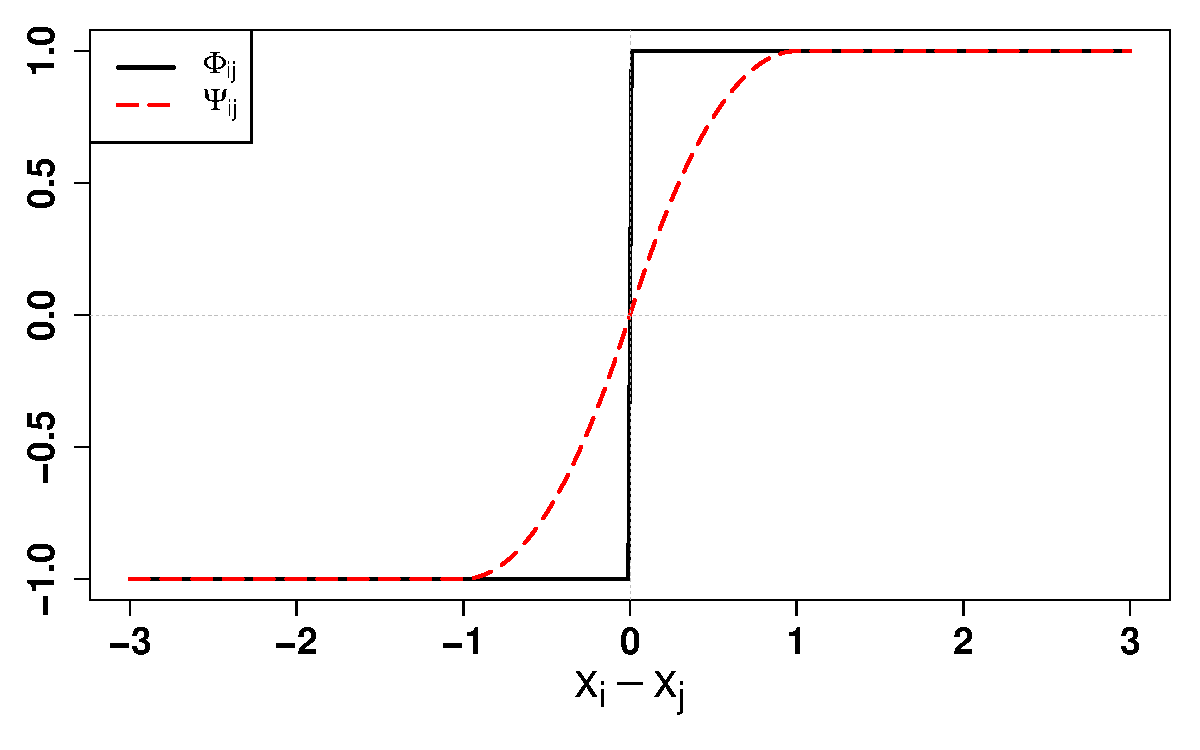
\includegraphics[width=0.6\textwidth]{ch-kendall/figures/smoothheaviside}
\caption{Smooth approximation (in red) of the Heaviside function (in black) used to define the mapping \eqref{eq2:smoothmap} for $a=1$.}
\label{fig2:smoothheaviside}
\end{center}
\end{figure} 


Although the smoothed kernel \eqref{eq2:G} can be an interesting alternative to the Kendall kernel \eqref{eq2:kdtALL}, we unfortunately lose for $G$ the computational trick that allows to compute $K_\tau$ in $O(n\log n)$. Specifically, we have two ways to compute $G$:

\noindent {\bf (i) Exact evaluation.} The first alternative is to compute explicitly the $n\choose 2$-vector representation $\Psi$ in the feature space, and then take the dot product to obtain $G$. While the kernel evaluation is exact, an analytic form of the smoothed mapping \eqref{eq2:Gkernel} is required and the computational cost is linear with the dimension of the feature space, i.e., $O(n^2)$.

\noindent {\bf (ii) Monte Carlo approximation.} The second alternative requires the observation that the smoothed mapping $\Psi(\xb) = \mathbb{E}\Phi(\tilde{\xb})$ appears in the form of expectation and can thus be  approximated by a $D$-sample mean of jittered points mapped by $\Phi$ into the feature space:
\begin{equation*}\label{eq2:mcpsi}
\Psi_D(\xb) = \frac{1}{D}\sum_{j=1}^D \Phi(\tilde{\xb}^j) \,,
\end{equation*}
where $\tilde{\xb}^1,\ldots,\tilde{\xb}^D$ are i.i.d. noisy versions of $\xb$. The dot product induces a kernel:
\begin{equation}\label{eq2:mc}
G_D(\xb,\xb') = \Psi_D(\xb)^\top \Psi_D(\xb') = \frac{1}{D^2} \sum_{i=1}^D \sum_{j=1}^D K_\tau\br{\tilde{\xb}^i , \tilde{\xb}'^j}\,,
\end{equation}
which is a $D^2$-sample empirical estimate of $G(\xb,\xb') = \mathbb{E} K_\tau(\tilde{\xb},\tilde{\xb}')$ when $\xb,\xb'$ are independently jittered with identically distributed noise. Since $K_\tau$ is of computational complexity $O(n\log n)$, computing $G_D$ requires $O(D^2 n \log n)$.


Note that the second alternative is faster to compute than the first one as long as, up to constants, $D^2 < n / \log n$, and small values of $D$ are thus favored on account of computational consideration. In that case, however, the approximation performance can be unappealing. To better understand the trade-off between the two alternatives, the question should be addressed upon how large $D$ should be so that the approximation error is not detrimental to the performance of a learning algorithm if we use the approximate kernel $G_D$ instead of $G$. Lemma \ref{lem2:concentration} provides a first answer to this question, showing that the approximation error of the kernel is upper bounded by $O(1/\sqrt{D})$ with high probability:
\begin{lemma}\label{lem2:concentration}
For any $0<\delta<1$, the following holds:

\noindent (a) For any $\xb\in\RR^n$, with probability greater than $1-\delta$,
$$
\nm{\Psi_D(\xb) - \Psi(\xb)} \leq \frac{1}{\sqrt{D}} \br{ 2+ \sqrt{8\log\frac{1}{\delta}}}\,.
$$

\noindent (b) For any $\xb_1, \ldots, \xb_m \in \RR^n$, with probability greater than $1-\delta$,
$$
\sup_{i=1,\ldots,m}\nm{\Psi_D(\xb_i) - \Psi(\xb_i)} \leq \frac{1}{\sqrt{D}} \br{ 2+ \sqrt{8\log\frac{m}{\delta}}}\,.
$$
\end{lemma}

\begin{proof}
For any $\xb\in\RR^n$, note that $\nm{\Phi(\xb)} \leq 1$. We can therefore apply \cite[Example 6.3]{Boucheron2013Concentration} to the random vector $X_j = \Phi(\tilde{\xb}^j) - \Psi(\xb)$ that satisfies $\EE X_j = 0$ and $\nm{X_j}\leq 2$ a.s. to get, for any $u\geq 2/\sqrt{D}$,
$$
\mathbb{P}\br{\nm{\Psi_D(\xb) - \Psi(\xb)} \geq u} \leq \exp \Bigg(-\frac{\br{u\sqrt{D}-2}^2}{8}\Bigg)\,.
$$
We recover (a) by setting the right-hand side equal to $\delta$ and solving for $u$. (b) then follows by a simple union bound.
\end{proof}

The uniform approximation bound of Lemma \ref{lem2:concentration} in turn implies that learning with the approximate kernel $G_D$ can be almost as good with the kernel $G$, as we now discuss. For that purpose, let us consider for example the case where the smoothed kernel $G$ is used to train a Support Vector Machine (SVM) from a training set $\mathcal{D}=\{(\mathbf{x}_i,y_i)\}_{i=1}^m\subset (\RR^n \times \{-1,+1\})^m$, specifically to estimate a function $h(\mathbf{x})=\mathbf{w}^\top \Psi(\mathbf{x})$ by solving
\begin{equation}
\label{eq2:svm}
\min_{\mathbf{w}} F(\mathbf{w})=\frac{\lambda}{2} \|\mathbf{w}\|^2 + \widehat{R}(\mathbf{w}),
\end{equation}
where $\widehat{R}(\mathbf{w})=\frac{1}{m}\sum_{i=1}^m \ell(y_i \mathbf{w}^\top \Psi(\mathbf{x}_i))$ is the empirical loss, with $\ell(y_i \mathbf{w}^\top \Psi(\mathbf{x}_i))=\max(0, 1-y_i \mathbf{w}^\top \Psi(\mathbf{x}_i))$ the hinge loss associated to the $i$-th point, $\lambda$ the regularization parameter. Now suppose that instead of training the SVM with smoothed feature mapping on the original points $\{\Psi(\xb_i)\}_{i=1,\dots,m}$, we first randomly jitter $\{\xb_i\}_{i=1,\dots,m}$ $D$ times at each point, resulting in $\{\tilde{\xb}_i^j\}_{i=1,\dots,m;j=1,\dots,D}$, and then replace each $\Psi(\xb_i)$ by the $D$-sample empirical average of jittered points mapped by $\Phi$ into the feature space, that is
$$
\Psi_D(\xb_i) := \frac{1}{D}\sum_{j=1}^D \Phi(\tilde{\xb}_i^j)\,.
$$
Note that $ \Psi_D(\xb_i)^\top \Psi_D(\xb_j)=G_D(\xb_i,\xb_j)$, hence training an SVM with the Monte Carlo approximate $G_D$ instead of exact version $G$ is equivalent to solving \eqref{eq2:svm} with $\{\Psi_D(\xb_i)\}_{i=1,\dots,m}$ in the hinge loss instead of $\{\Psi(\xb_i)\}_{i=1,\dots,m}$. Theorem \ref{thm2:approx} quantifies the approximation performance in terms of objective function $F$ which helps to answer the question on the trade-off between $G$ and $G_D$ in computational complexity and learning accuracy.


\begin{thm}\label{thm2:approx}
For any $0\leq\delta\leq 1$, the solution $\wh_D$ of the SVM trained with the Monte Carlo approximation \eqref{eq2:mc} with $D$ random-jittered samples for each training point satisfies, with probability greater than $1-\delta$,
$$
F(\wh_D) \leq \min_{\mathbf{w}} F(\mathbf{w}) +  \sqrt{\frac{8}{\lambda D}} \br{ 2+ \sqrt{8\log\frac{m}{\delta}}}\,.
$$
\end{thm}

\begin{proof}
Let $\wh$ be a solution to the original SVM optimization problem, and $\wh_D$ a solution to the perturbed SVM, i.e., a solution of
\begin{equation}
\label{eq2:svmD}
\min_{\mathbf{w}} F_D(\mathbf{w})=\frac{\lambda}{2} \|\mathbf{w}\|^2 + \widehat{R}_D(\mathbf{w}),
\end{equation}
with $\widehat{R}_D(\mathbf{w})=\frac{1}{m}\sum_{i=1}^m \ell(y_i \mathbf{w}^\top \Psi_D(\mathbf{x}_i))$. Since the hinge loss is $1$-Lipschitz, i.e., $|\ell(a)-\ell(b)|\leq |a-b|$ for any $a,b\in\RR$, we obtain that for any $\ub\in\RR^{n\choose 2}$: 
\begin{equation}\label{eq2:risklipschitz}
\begin{split}
\abs{\Rh(\ub)-\Rh_D(\ub)} &\leq \frac{1}{m}\sum_{i=1}^m \abs{\ub^\top\br{\Psi(\xb_i) - \Psi_D(\xb_i)}} \\
& \leq \nm{\ub} \sup_{i=1,\ldots,m}\nm{\Psi_D(\xb_i) - \Psi(\xb_i)}\,.
\end{split}
\end{equation}
Now, since $\wh_D$ is a solution of \eqref{eq2:svmD}, it satisfies
$$
\nm{\wh_D} \leq \sqrt{\frac{2F_D(\wh_D)}{\lambda}} \leq \sqrt{\frac{2F_D(0)}{\lambda}} = \sqrt{\frac{2}{\lambda}}\,,
$$
and similarly $\nm{\wh} \leq \sqrt{2/\lambda}$ because $\wh$ is a solution of the original SVM optimization problem. Using \eqref{eq2:risklipschitz} and these bounds on $\nm{\wh_D}$ and $\nm{\wh}$, we get
\begin{equation*}
\begin{split}
F(\wh_D) & - F(\wh) \\
& = F(\wh_D) - F_D(\wh_D) + F_D(\wh_D) - F(\wh)\\
&\leq F(\wh_D) - F_D(\wh_D) + F_D(\wh) - F(\wh)\\
&= \Rh(\wh_D)-\Rh_D(\wh_D) + \Rh_D(\wh) -\Rh(\wh)\\
& \leq \br{\nm{\wh_D} + \nm{\wh}} \sup_{i=1,\ldots,m}\nm{\Psi_D(\xb_i) - \Psi(\xb_i)}\\
& \leq \sqrt{\frac{8}{\lambda}} \sup_{i=1,\ldots,m}\nm{\Psi_D(\xb_i) - \Psi(\xb_i)} \,.
\end{split}
\end{equation*}
Theorem \ref{thm2:approx} then follows from Lemma \ref{lem2:concentration}.
\end{proof}


It is known that compared to the exact solution of \eqref{eq2:svm}, an $O(m^{-1/2})$-approximate solution is sufficient to reach the optimal statistical accuracy \cite{Bottou2008Tradeoffs}. This accuracy can be attained in our analysis when $D = O(m/\lambda)$, and since typically $\lambda \sim m^{-1/2}$ \cite{Steinwart2005Consistency}, this suggests that it is sufficient to take $D$ of order $m^{3/2}$. Going back to the comparison strategy of the two alternatives $G$ and $G_D$, we see that the computational cost of computing the full $m\times m$ Gram matrix with the exact evaluation is $O(m^2 n^2)$, while the cost of computing the approximate Gram matrix with $D=O(m^{3/2})$ random samples is $O(m^2 D^2 n \log n) = O(m^5 n \log n)$. This shows that, up to constants and logarithmic terms, the Monte Carlo approximation is interesting when $m = o(n^{1/3})$, otherwise the exact evaluation using explicit computation in the feature space is preferable.

Interestingly we can look at the extended Kendall kernel \eqref{eq2:G} to uncertain rankings from the perspective of Hilbert space embeddings of probability distributions \cite{Smola2007Hilbert}. In fact, for $x$ fixed, the smoothed mapping $\Psi(\xb) = \EE \Phi(\xb+\epsilon)$ is exactly an embedding for the distribution $\mathcal{P}$ of an additive noise $\epsilon$ in the reproducing kernel Hilbert space (RKHS) associated with Kendall kernel. As a consequence, the idea of smoothed kernel $G(\xb,\xb')$ for $\xb,\xb'\in \mathcal{X}$ is essentially equivalent to how \cite[Lemma 4]{Muandet2012Learning} defines kernels on two probability distributions from $\{\mathcal{P}+\xb | \xb \in \mathcal{X} \}$ using the Kendall kernel as the level-1 embedding kernel and linear inner product as the level-2 kernel in the feature space. As a result, given a fixed training set $\mathcal{D}$, training an SVM with $G$ in place of $K_\tau$ is equivalent to training a Flex-SVM instead of an ordinary SVM with $K_\tau$ \cite{Muandet2012Learning}. In this case, Theorem \ref{thm2:approx} provides an error bound in terms of the optimal accuracy for cases when training a Flex-SVM if exact evaluation of $G$ is intractable and its Monte Carlo approximate $G_D$ is employed. This serves to obtain a trade-off between computation complexity and approximation accuracy which is particularly interesting when we are working in high dimensions.








\section{Relation of the Mallows Kernel and the Diffusion Kernel on $\mathbb{S}_n$}
\label{sec2:group}

It is interesting to relate the Mallows kernel \eqref{eq2:mallows} to the diffusion kernel on the symmetric group proposed by \cite{Kondor2010Ranking}, which is the diffusion kernel \cite{Kondor2002Diffusion} on the Cayley graph of $\Sn$ generated by adjacent transpositions with left-multiplication. This graph, illustrated for a specific case of $n=4$ in Figure \ref{fig2:permutahedron}, is defined by $\mathcal{G}=(\mathcal{V},\mathcal{E})$ with $\mathcal{V}=\mathbb{S}_n$ as vertices, and undirected edge set $\mathcal{E}=\big\{ \{\sigma,\pi\sigma\} : \sigma\in \mathbb{S}_n,\pi\in Q \big\}$, where $Q=\{(i,i+1)|i=1,\dots,n-1\}$ the set of all adjacent transpositions. Note $Q$ is symmetric in the sense that $\pi\in Q \Leftrightarrow \pi^{-1}\in Q$, and the graph adjacency relation is a right-invariant relation, that is $\sigma \sim \sigma' \Leftrightarrow \sigma'\sigma^{-1}\in Q$. The corresponding graph Laplacian is the matrix $\Delta$ with
\begin{equation*}
	\Delta_{\sigma,\sigma'} = \left\{
		\begin{array}{ll}
			1 & \textrm{if } \sigma \sim \sigma' \\
			-(n-1) & \textrm{if } \sigma = \sigma' \\
			0 & \textrm{otherwise}
		\end{array}
	\right. ,
\end{equation*}
where $n-1$ is the degree of vertex $\sigma$ (number of edges connected with vertex $\sigma$), and the \emph{diffusion kernel} on $\Sn$ is finally defined as
\begin{equation}
	\label{eq2:diffusionkernel}
	K_{\textrm{dif}}^{\beta} (\sigma,\sigma') = [e^{\beta \Delta}]_{\sigma,\sigma'}
\end{equation}
for some diffusion parameter $\beta \in \mathbb{R}$, where $e^{\beta \Delta}$ is the matrix exponential. $K_{\textrm{dif}}^{\beta}$ is a right-invariant kernel on the symmetric group \cite[Proposition 2]{Kondor2010Ranking}, and we denote by $\kappa_{\textrm{dif}}^\beta$ the positive definite function induced by $K_{\textrm{dif}}^{\beta}$ such that $K_{\textrm{dif}}^{\beta}(\sigma,\sigma') = \kappa_{\textrm{dif}}^\beta (\sigma'\sigma^{-1}).$ Since the Mallows kernel $K_M^\lambda$ is straightforwardly right-invariant, we denote by $\kappa_M^\lambda$ the positive definite function induced by the Mallows kernel $K_M^\lambda$ such that $K_M^\lambda(\sigma,\sigma') = \kappa_M^\lambda (\sigma'\sigma^{-1}).$ One way to interpret the diffusion kernel \eqref{eq2:diffusionkernel} is by the heat equation on the Cayley graph
\begin{equation*}
	\frac{d}{d \beta} K_{\textrm{dif}}^{\beta} = \Delta K_{\textrm{dif}}^{\beta} \quad \mbox{ s.t. } K_{\textrm{dif}}^{\beta}|_{\beta=0}=I.
\end{equation*}
$K_{\textrm{dif}}^{\beta}$ is thus the product of a continuous process, expressed by the graph Laplacian $\Delta$, gradually transforming local structure $K_{\textrm{dif}}^{\beta}|_{\beta=0}=I$ to a kernel with stronger and stronger off-diagonal effects as $\beta$ increases.





\begin{figure}[!htbp]
\begin{center}
\centerline{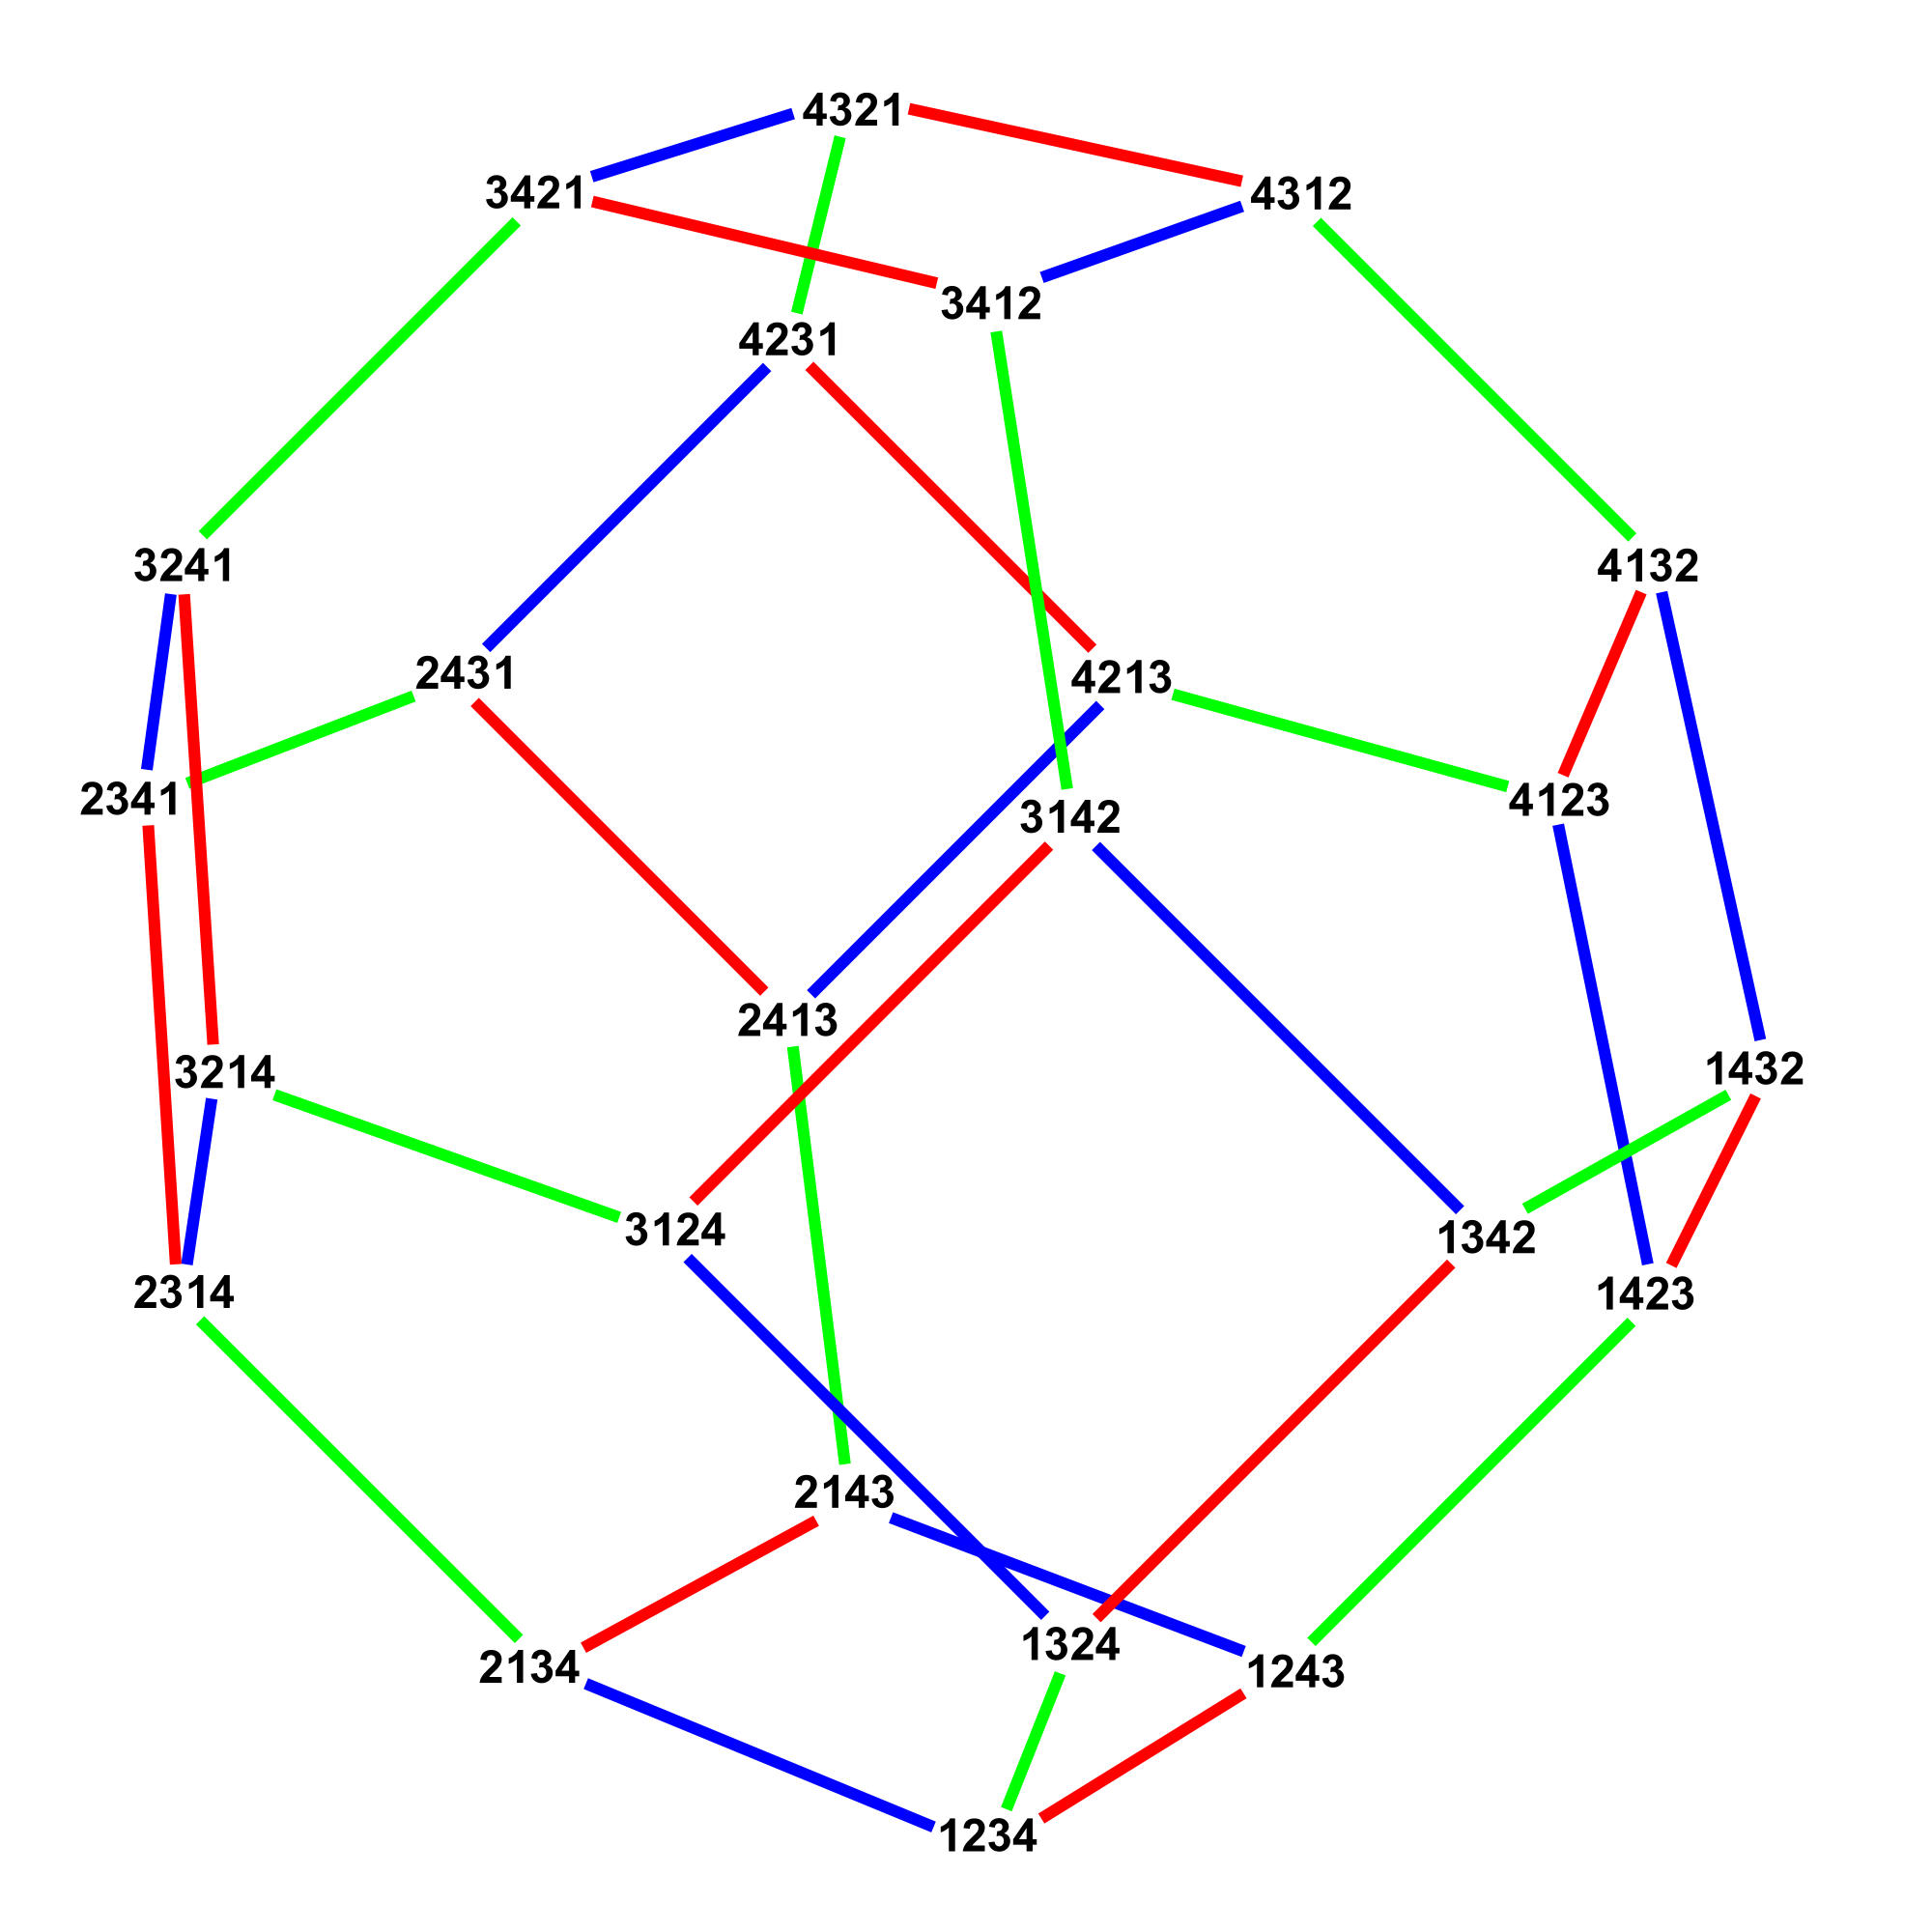
\includegraphics[width=0.6\textwidth]{ch-kendall/figures/permutahedron}}
\caption{Cayley graph of $\mathbb{S}_4$, generated by the transpositions (1 2) in blue, (2 3) in green, and (3 4) in red.}
\label{fig2:permutahedron}
\end{center}
\end{figure} 




Interestingly, the Mallows kernel can also be interpreted with the help of the Cayley graph. Indeed, it is well-known that the Kendall tau distance $n_d(\sigma,\sigma')$ is the minimum number of adjacent swaps required to bring $\sigma$ to $\sigma'$, i.e. $n_d(\sigma,\sigma')$ equals to the shortest path distance on the Cayley graph \cite[Exercise 7.73]{Drutu2017Geometric}, or simply written
\begin{equation*}
n_d(\sigma,\sigma')=d_{\mathcal{G}}(\sigma,\sigma') \,.
\end{equation*}
Different from the diffusion kernel for which communication between permutations is a diffusion process over the graph, the Mallows kernel 
$$K_{M}^{\lambda}(\sigma,\sigma')=e^{-\lambda n_d(\sigma,\sigma')}=e^{-\lambda d_{\mathcal{G}}(\sigma,\sigma')}$$ 
considers exclusively the shortest path over the graph when expressing the similarity between permutations $\sigma,\sigma'$. 






A notable advantage of the Mallows kernel over the diffusion kernel is that the Mallows kernel enjoys faster evaluation. On one hand if data instances are total rankings, i.e. $\sigma,\sigma'\in \mathbb{S}_n$, evaluating $K_{\textrm{dif}}^{\beta}(\sigma,\sigma')$ would require exponentiating an $n!$-dimensional Laplacian matrix by naive implementation, and can reduce to exponentiating matrices of smaller sizes by careful analysis in the Fourier space, which still remains problematic if working dimension $n$ is large \cite{Kondor2010Ranking}. However, evaluating $K_{M}^{\lambda}(\sigma,\sigma')$ only takes $O(n\log n)$ time. On the other hand if data instances are partial ranking of size $k\ll n$, i.e. $R,R'\subset \mathbb{S}_n$, and we take convolution kernel \eqref{eq2:partialranking} to extend the two kernels, the analysis of exploring the sparsity of the Fourier coefficients of the group algebra of partial rankings $R,R'$ of size $k$ reduces the evaluation of both the diffusion kernel and the Mallows kernel to $O((2k)^{2k+3})$ time, provided that the exponential kernel Fourier matrices $[\hat{\overline{\kappa}}(\mu)]_{\geq [\dots]_{n-k}}$ are precomputed before any kernel evaluations take place \cite[Theorem 13]{Kondor2010Ranking}.









\section{Application: Clustering and Modeling Rank Data}
\label{sec2:clustering}

In this section we illustrate the potential benefit of kernel-based algorithms using the Kendall and Mallows kernels for the purpose of unsupervised cluster analysis, i.e., partitioning a collection of rank data into sub-groups and/or estimating densities of a collection of rank data. This is in particular of great practical interest in social choice theory in order to explore the heterogeneity and identify typical sub-groups of voters with a common behavior to understand, for example, their political support for various parties \cite{Gormley2006Analysis,Gormley2008Exploring,Marden1996Analyzing}.


\subsection{Clustering with Kernel $k$-means}
\label{sec2:clusterkmeans}

Let $\cbr{\sigma_i}_{i=1}^m \subset \Sn$ be a collection of $m$ permutations representing, say, the preferences of customers over $n$ products or the votes of electorate over $n$ candidates. We aim at partitioning these permutations into $c \leq m$ clusters $\cbr{S_j}_{j=1}^c$. One approach to cluster rank data is to follow a method similar to $k$-means in the symmetric group. Assuming that each cluster $S_j$ has a ``center'' $\pi_j \in\Sn$ serving as a prototype permutation of that cluster, the classic $k$-means clustering attempts to put each point in the cluster with the nearest center so as to minimize the sum of Kendall tau distance of each permutation to the corresponding center of its cluster. Specifically, when the number of clusters $c$ is fixed, the objective is to find:
\begin{equation}\label{eq2:kmeans}
\underset{\cbr{S_j,\pi_j\in\Sn}}{\arg\min} \sum_{j=1}^c \sum_{i:\sigma_i\in S_j} n_d(\sigma_i,\pi_j) \,.
\end{equation}
Note that \eqref{eq2:kmeans} reduces to a single-ranking aggregation problem when $c=1$, where the center $\pi$ is commonly known as Kemeny consensus \cite{Kemeny1962Mathematical} which is NP-hard to find \cite{BartholdiIII1989Voting}. With the objective in \eqref{eq2:kmeans} being non convex, Lloyd's algorithm is usually employed to find local minima in an iterative manner consisting of two steps: the \emph{assignment step} assigns each point to its closest cluster, and the \emph{update step} updates each of the $c$ cluster centers using the points assigned to that cluster; the algorithm repeats until all the cluster centers remain unchanged in an iteration. While the assignment step is usually fast, the update step is indeed equivalent to solving a Kemeny consensus problem for each cluster, i.e., $\arg\min_{\pi_j\in\Sn} \sum_{i:\sigma_i\in S_j} n_d(\sigma_i,\pi_j)$. Since the exact Kemeny-optimal ranking is difficult to find, approximate techniques are usually employed in practice such as Borda Count \cite{Borda1781Memoire} or Copeland's method \cite{Copeland1951reasonable}.

As the Kendall tau distance is conditionally positive definite, we can propose as an alternative to use the kernel $k$-means approach \cite{Girolami2002Mercer,Zhang2002large} that relaxes the assumption that the cluster center are permutations, and instead works implicitly in the feature space where cluster centers can be any vector in $\RR^{{n\choose 2}}$ by considering the problem:
\begin{equation*}\label{eq2:kernelkmeans}
\underset{\big\{S_j,\mu_j\in\RR^{{n\choose 2}}\big\}}{\arg\min} \sum_{j=1}^c \sum_{i:\sigma_i\in S_j} \nm{\Phi(\sigma_i) - \mu_j}^2 \,,
\end{equation*}
for which local minima can be found efficiently by Algorithm \ref{alg:kernelkmeans}. Note that $\mu_j$ does not match a true permutation $\pi_j\in\Sn$ in general, and the Kemeny consensus problem in the update step is thus bypassed. It is worthwhile to note that the algorithm is not exclusive for clustering permutations, kernel $k$-means clustering can be applied respectively to total/partial/multivariate/uncertain rankings with appropriate kernels defined.

\begin{algorithm}[!htbp]
\caption{Kernel $k$-means for clustering heterogeneous rank data.}
{\bfseries Input:} a collection of permutations $\cbr{\sigma_i}_{i=1}^m$ and a kernel function $K$ over $\Sn$, or a kernel matrix evaluated between pairwise data points $\mathbf{K} = (K(\sigma_i,\sigma_j))_{1 \leq i,j \leq m}$; the number of clusters $c\leq m$.
\begin{algorithmic}[1]
 \STATE Randomly initialize cluster assignment for each data points and form $c$ clusters $S_1,\dots,S_c$.
 \STATE For each data point, find its new cluster assignment, i.e., for $i=1,\dots,m,$ 
 	$$j^*(\sigma_i) = \arg\min_j d_{ij} \,,$$
 	where
 	\begin{multline*}
 	d_{ij} := \nm{\Phi(\sigma_i) - \frac{1}{|S_j|} \sum_{\sigma_\ell\in S_j} \Phi(\sigma_\ell)}^2 \\
 	= K(\sigma_i,\sigma_i) - \frac{2}{|S_j|} \sum_{\sigma_\ell\in S_j} K(\sigma_i,\sigma_\ell)
 	+ \frac{1}{|S_j|^2} \sum_{\sigma_v,\sigma_\ell\in S_j} K(\sigma_v,\sigma_\ell) \,.
 	\end{multline*}
 \STATE Form updated clusters, i.e., for $j=1,\dots,c,$ 
 	$$S_j=\cbr{\sigma_i : j = j^*(\sigma_i), i=1,\dots,m} \,.$$
 \STATE Repeat 2-3 until all cluster assignments remain unchanged in an iteration.
\end{algorithmic}
{\bfseries Output:} Cluster assignments $\cbr{S_j}_{j=1}^c.$
\label{alg:kernelkmeans}
\end{algorithm}



\subsection{Mallows Mixture Model with Kernel Trick}
\label{sec2:clustermallows}

An alternative to $k$-means clustering is to consider mixture models, which provide a method for modeling heterogeneous population in data by assuming a mixture of standard models for rankings in each homogeneous sub-population. Mixture models not only allow to cluster data, but more generally to estimate a distribution on the space of permutation that can then be used for other purposes, such as combining evidences. One popular choice of probabilistic distribution over $\Sn$ is the Mallows model \cite{Mallows1957Non}, which takes the form in expressing the occurring probability of $\sigma$ by 
\begin{equation}\label{eq2:mallowspdf}
f(\sigma|\pi,\lambda) = C(\lambda) \exp[-\lambda n_d(\sigma,\pi)] \,,
\end{equation}
where the central ranking $\pi\in\Sn$ and the precision $\lambda\geq 0$ are model parameters, and the normalization constant $C(\lambda) = 1 / \sum_{\sigma'\in\Sn} \exp[-\lambda n_d(\sigma',\pi)]$ is chosen so that $f(\cdot|\pi,\lambda)$ is a valid probability mass function over $\Sn$. Notably, $C(\lambda)$ does not depend on the center $\pi$ due to the symmetry of $\Sn$. 


We follow the mixture modeling setup in \cite{Murphy2003Mixtures}. Now suppose that a population consists of $c$ sub-populations, a Mallows mixture model assumes that an observation comes from group $j$ with probability $p_j\geq 0$ for $j=1,\dots,c$ and, given that the observation belongs to sub-population $j$, it is generated from a Mallows model with central ranking $\pi_j$ and precision $\lambda_j$, i.e., the occurring probability of $\sigma$ in the Mallows mixture model is written as
\begin{equation}\label{eq2:mallowsf}
f(\sigma) = \sum_{j=1}^c p_j f(\sigma|\pi_j,\lambda_j) = \sum_{j=1}^c p_j C(\lambda_j) \exp[-\lambda_j n_d(\sigma,\pi_j)] \,.
\end{equation}
Denoting $\underline{\pi} = \cbr{\pi_j}_{j=1}^c$, $\underline{\lambda}=\cbr{\lambda_j}_{j=1}^c$, $\underline{p}=\cbr{p_j}_{j=1}^c$ such that $\sum_{j=1}^c p_j=1$, the log-likelihood of a collection of $m$ i.i.d. permutations $\underline{\sigma}=\cbr{\sigma_i}_{i=1}^m$ is therefore:
\begin{equation}\label{eq2:mallowsL}
L(\underline{\pi},\underline{\lambda},\underline{p}|\underline{\sigma}) = \sum_{i=1}^m \log f(\sigma_i)
= \sum_{i=1}^m \log \cbr{\sum_{j=1}^c p_j C(\lambda_j) \exp[-\lambda_j n_d(\sigma_i,\pi_j)]} \,.
\end{equation}
The Mallows mixture model is usually fitted by maximum likelihood using the EM algorithm. Specifically, by introducing latent (membership) variables $\underline{z} = \cbr{z_{ij}:i=1,\dots,m,j=1,\dots,c}$ where $z_{ij} = 1$ if $\sigma_i$ belongs to group $j$ and $0$ otherwise, the complete log-likelihood of data is
\begin{equation*}
L_C(\underline{\pi},\underline{\lambda},\underline{p}|\underline{\sigma},\underline{z}) = \sum_{i=1}^m \sum_{j=1}^c z_{ij}[\log p_j + \log C(\lambda_j) - \lambda_j n_d(\sigma_i,\pi_j)] \,.
\end{equation*}
The EM algorithm can be implemented to find local maximum likelihood estimates following two steps iteratively until convergence: the \emph{E-step} calculates the expected value of membership variables $\underline{\hat{z}}$ conditioned on the current estimates of the model parameters $\underline{\pi},\underline{\lambda},\underline{p}$, and the \emph{M-step} updates the model parameters $\underline{\pi},\underline{\lambda},\underline{p}$ by maximizing the expected complete log-likelihood $\hat{L}_C = L_C(\underline{\pi},\underline{\lambda},\underline{p}|\underline{\sigma},\underline{\hat{z}})$ where membership variables are replaced by their expected values. The final estimate $\hat{z}_{ij}$ amounts to our belief of $\sigma_i$ belonging to group $j$, and can thus be used to form clusters $\cbr{S_j}_{j=1}^c$ serving a partition of data where
\begin{equation}\label{eq2:mallowscluster}
S_j=\cbr{\sigma_i : \hat{z}_{ij} = \max_{\ell} \hat{z}_{i\ell}, i=1,\dots,m} \,.
\end{equation}


A closer look at the EM algorithm reveals that optimizing $\hat{L}_C$ with respect to $\underline{\pi}$ alone in the M-step is indeed equivalent to finding a (weighted) Kemeny consensus for each group, i.e., solving $\arg\min_{\pi_j\in\Sn} \sum_{i=1}^m \hat{z}_{ij} n_d(\sigma_i,\pi_j),$ for which exact solution is difficult as above-mentioned in the context of $k$-means clustering. Similarly to the idea of kernel $k$-means in contrast to classic $k$-means, we propose to seek ways to bypass the Kemeny consensus problem by working in the feature space instead. Note that the Mallows probability mass function \eqref{eq2:mallowspdf} is equivalently written as $f(\sigma|\pi,\lambda) \propto \exp \sqb{-\lambda \nm{\Phi(\sigma)-\Phi(\pi)}^2}$ up to a constant scaling on $\lambda$ by using \eqref{eq2:distance}, we propose to relax the constraint that the center has to match a true permutation $\pi\in\Sn$ and consider the following two alternatives in place of $f$ following the mixture modeling approach stated above:

\noindent {\bf (i) Kernel Mallows.} The Mallows probability mass function over $\Sn$ \eqref{eq2:mallowspdf} is generalized to admit any point in the feature space $\mu\in\RR^{{n\choose 2}}$ to be the population center, i.e.,
\begin{equation}\label{eq2:kernelmallows}
g(\sigma|\mu,\lambda) = C(\mu,\lambda) \exp \sqb{-\lambda \nm{\Phi(\sigma)-\mu}^2} \,,
\end{equation}
where the normalization constant $C(\mu,\lambda) = 1 / \sum_{\sigma'\in\Sn} \exp \sqb{-\lambda \nm{\Phi(\sigma')-\mu}^2}$ is chosen so that $g(\cdot|\mu,\lambda)$ is a valid probability mass function over $\Sn$. Notably, $C(\mu,\lambda)$ now depends on the center $\mu$ as well.

If we replace the probability mass function of classic Mallows $f$ in \eqref{eq2:mallowsL} by that of kernel Mallows $g$, the Kemeny consensus problem is averted when the EM algorithm is used to fit a local maximum likelihood estimate. However, another computational setback arises that the expected complete log-likelihood $\hat{L}_C$ to maximize in the M-step of the EM algorithm is separately concave with respect to $\mu$ or $\lambda$, but not jointly concave. Hence alternating optimization is often used in practice with the caveats of intensive computation and no guarantee to attain global optima for the M-step optimization at each iteration.


\noindent {\bf (ii) Kernel Gaussian.} Note that \eqref{eq2:kernelmallows} has a similar form to the Gaussian density, therefore we consider for $\sigma\in\Sn$,
\begin{equation}\label{eq2:kernelgaussian}
g^{\dagger} (\sigma|\mu,\lambda) = \sqrt{\br{\frac{\lambda}{\pi}}^{{n\choose 2}}} \exp \sqb{-\lambda \nm{\Phi(\sigma)-\mu}^2} \,,
\end{equation}
which is exactly $\mathcal{N}(\Phi(\sigma) | \mu, (2\lambda)^{-1} I )$, i.e., the ${n\choose 2}$-dimensional Gaussian distribution with mean $\mu$ and isotropic covariance matrix $(2\lambda)^{-1} I$ injected by $\Phi(\sigma)$. Notably, $g^{\dagger} (\cdot|\mu,\lambda)$ is not a valid probability mass function over $\Sn$.

The mixture modeling approach stated above using $g^{\dagger}$ instead of $f$ is in fact equivalently stated in Algorithm \ref{alg:kernelgaussian}. It is worthwhile to note that the algorithm also applies to total/partial/multivariate/uncertain rankings with appropriate kernels defined as \cite[Table 2]{Wang2003Kernel} provides the counterpart of Algorithm \ref{alg:kernelgaussian} in case that a kernel matrix evaluated between data points is given instead. However, since $g^{\dagger}$ itself is not a valid probability mass function over $\Sn$, an evident drawback is that we now lose the probabilistic interpretation of the mixture distribution as in \eqref{eq2:mallowsf}.


\begin{algorithm}[!htbp]
\caption{Kernel trick embedded Gaussian mixture model for clustering heterogeneous rank data.}
{\bfseries Input:} a collection of permutations $\cbr{\sigma_i}_{i=1}^m$ and a kernel function $K$ over $\Sn$; the number of clusters $c\leq m$.
\begin{algorithmic}[1]
 \STATE Compute feature points $\Phi(\sigma_i) \in \RR^{{n \choose 2}}$ mapped by the Kendall embedding.
 
 \STATE Fit a Gaussian mixture model for $\cbr{\Phi(\sigma_i)}_{i=1}^m$ in $\RR^{{n \choose 2}}$ using maximum likelihood with the EM algorithm under the constraint of isotropic covariance matrix, i.e., $\Sigma=(2\lambda)^{-1}I$.
 
 \STATE Use the membership estimates $\underline{\hat{z}}$ to form clusters by \eqref{eq2:mallowscluster}.
\end{algorithmic}
{\bfseries Output:} Cluster assignments $\cbr{S_j}_{j=1}^c.$
\label{alg:kernelgaussian}
\end{algorithm}



\subsection{Experiments}
\label{sec2:clusterexp}


\noindent {\bf Clustering 1980 APA election data.} In the 1980 American Psychological Association (APA) presidential election, voters were asked to rank $5$ candidates in order of preference, and $5738$ votes in form of total rankings were reported and thus used in our experiment. The dataset was thoroughly studied by \cite{Diaconis1988Group}.



We first use $k$-means approaches to cluster the data. We compare the proposed kernel $k$-means algorithm (Algorithm \ref{alg:kernelkmeans} with Kendall kernel $K_{\tau}$) to the classic $k$-means algorithm formulated as \eqref{eq2:kmeans}. For the classic $k$-means where cluster centers are required to be a prototype permutation, three methods are employed in the center-update step for each iteration: brute-force search of Kemeny-optimal ranking, approximate ranking induced by Borda Count and Copeland's method. In each case, we vary the number of clusters ranging from $2$ to $10$ and the algorithm is repeated $50$ times with randomly initialized configurations for each fixed number of clusters. We observe from Figure \ref{fig2:kmeans-time} that the kernel $k$-means or classic $k$-means with approximate centers runs much faster than optimal $k$-means for which the Kemeny-optimal ranking is time-consuming to find by a brute-force search. Further, Figure \ref{fig2:kmeans-silhouette} shows that the kernel $k$-means outperforms all three methods based on classic $k$-means in terms of the average silhouette scores of the clustering results, which justifies that the kernel $k$-means splits the data into more consistent sub-groups in the sense that instances, measured by Kendall tau distance on average, are more similar in the same cluster and more dissimilar in different clusters.



\begin{figure}[!htbp]
\centering
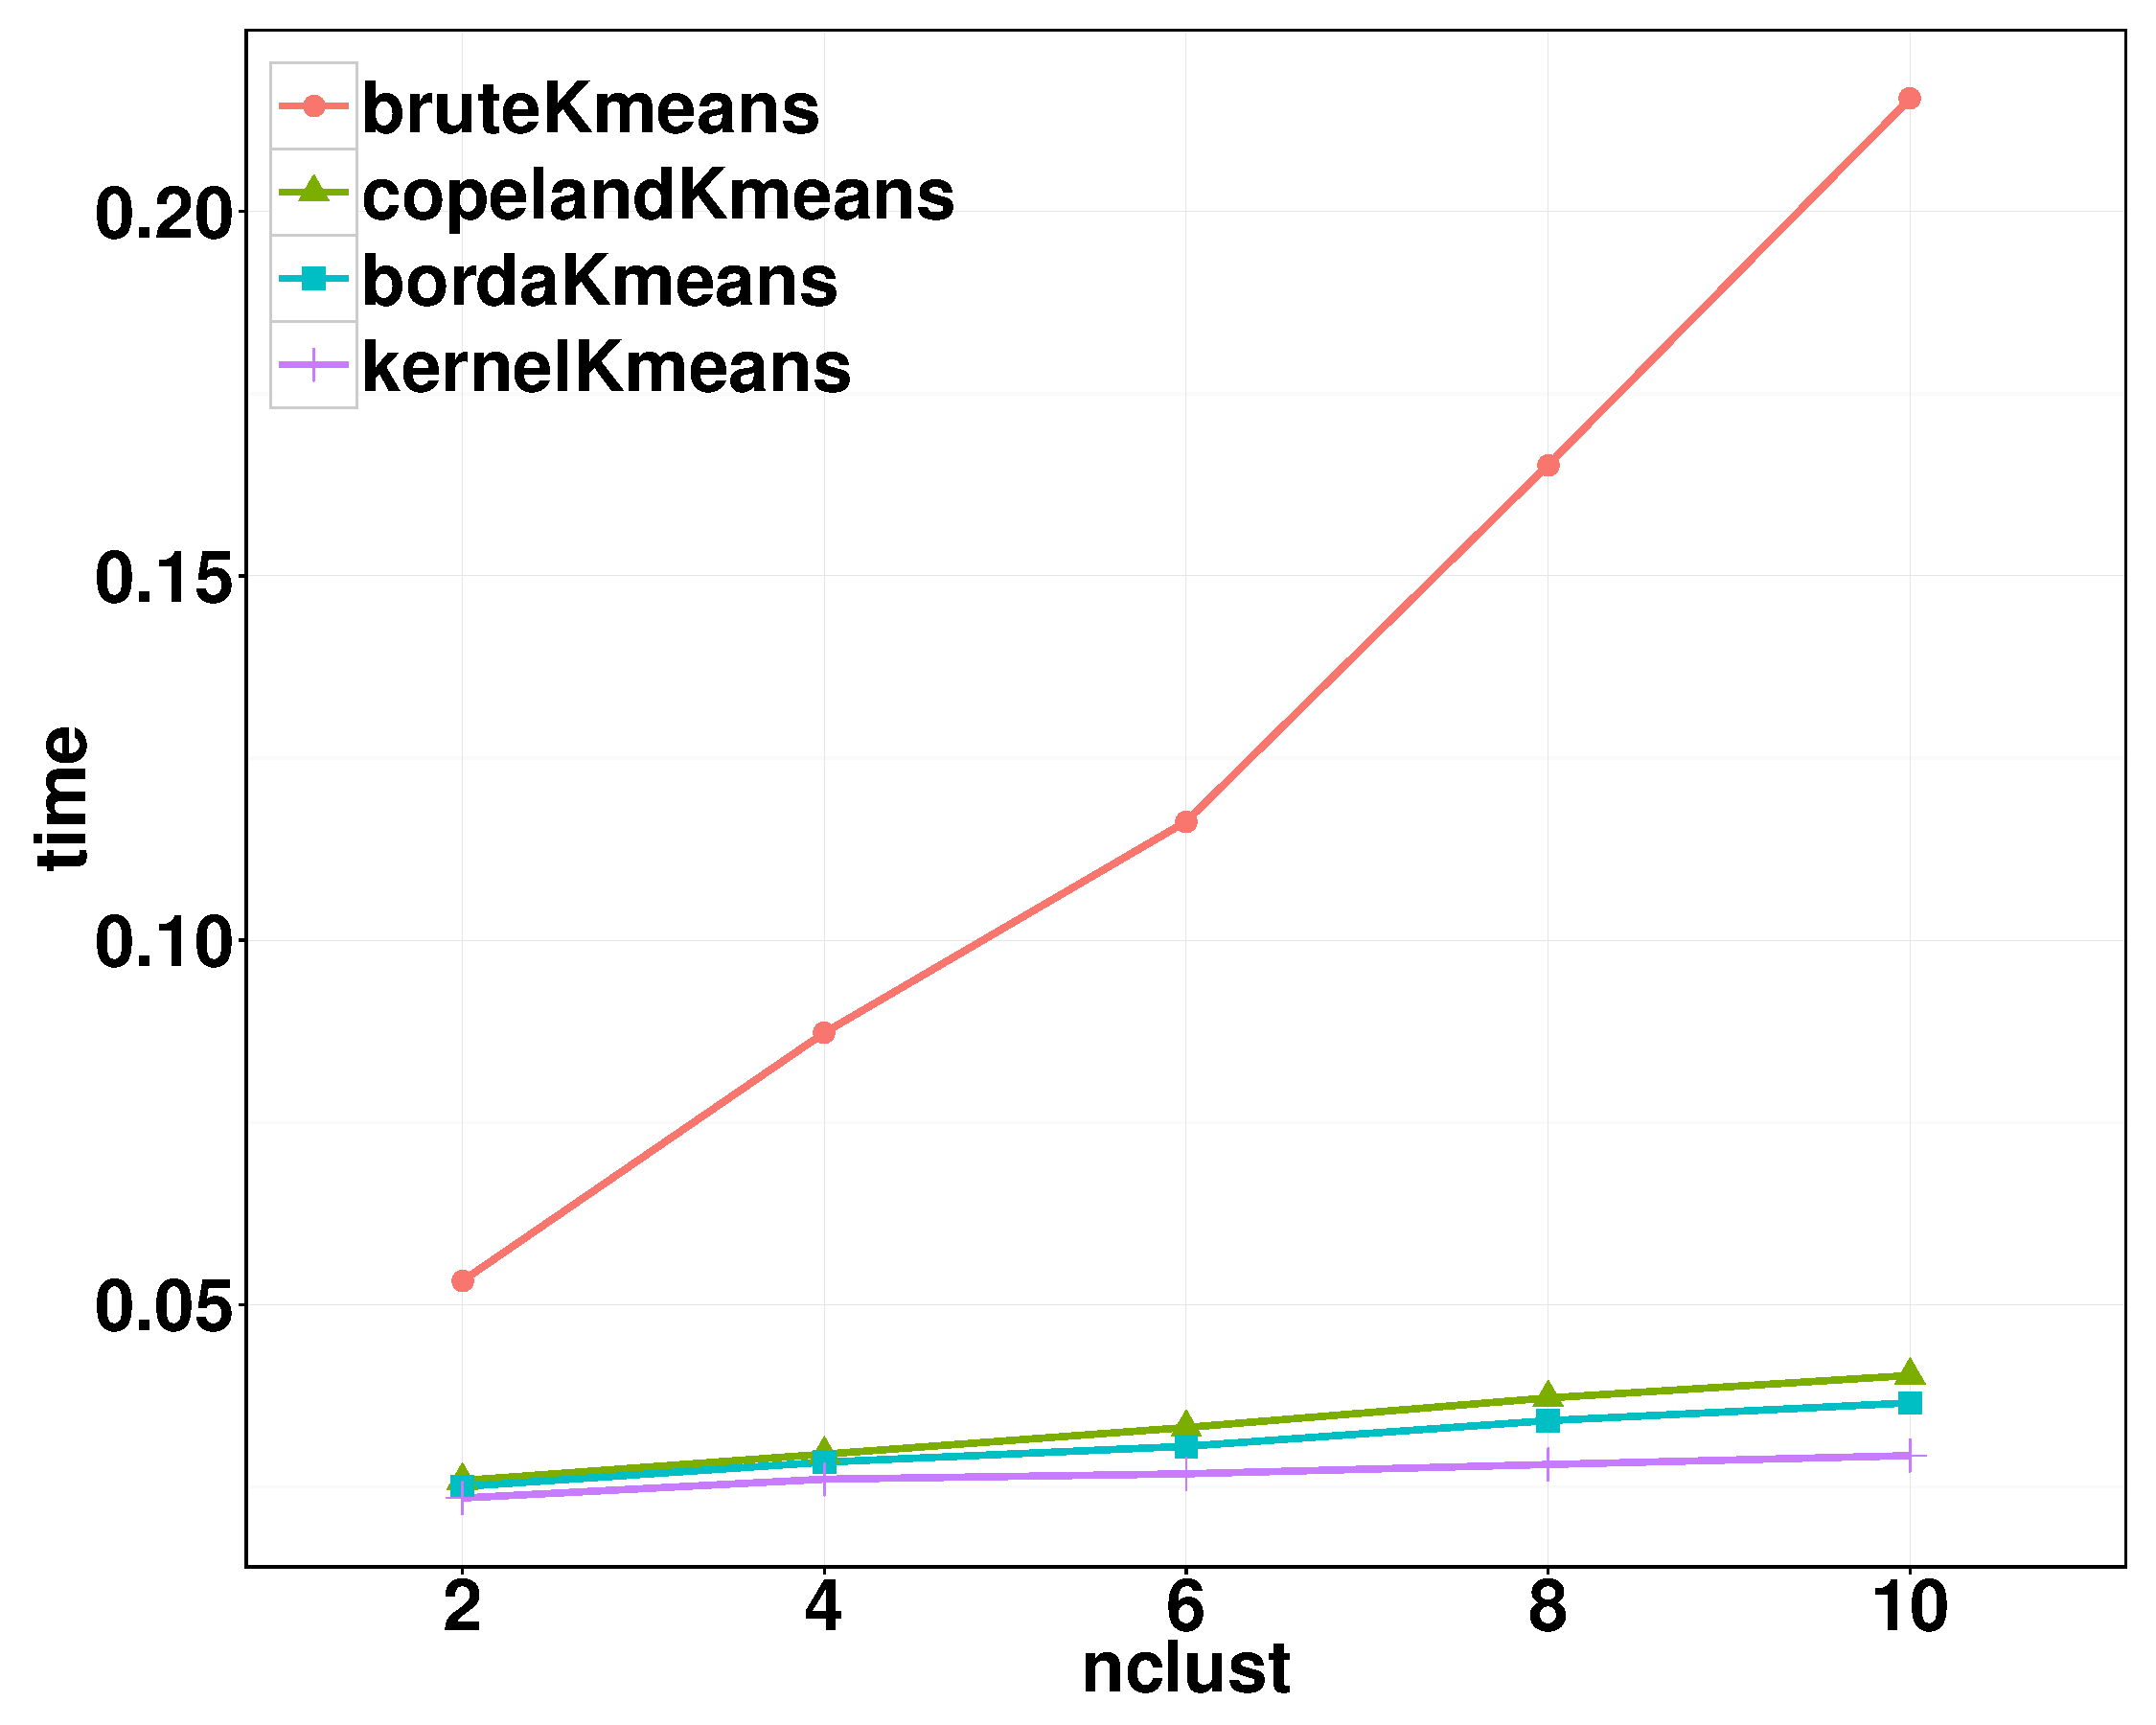
\includegraphics[width=0.6\textwidth]{ch-kendall/cluster_results/kmeans-time}\caption{Computational time (in seconds) of $k$-means algorithms per run across different number of clusters.}
\label{fig2:kmeans-time}
\end{figure}

\begin{figure}[!htbp]
\centering
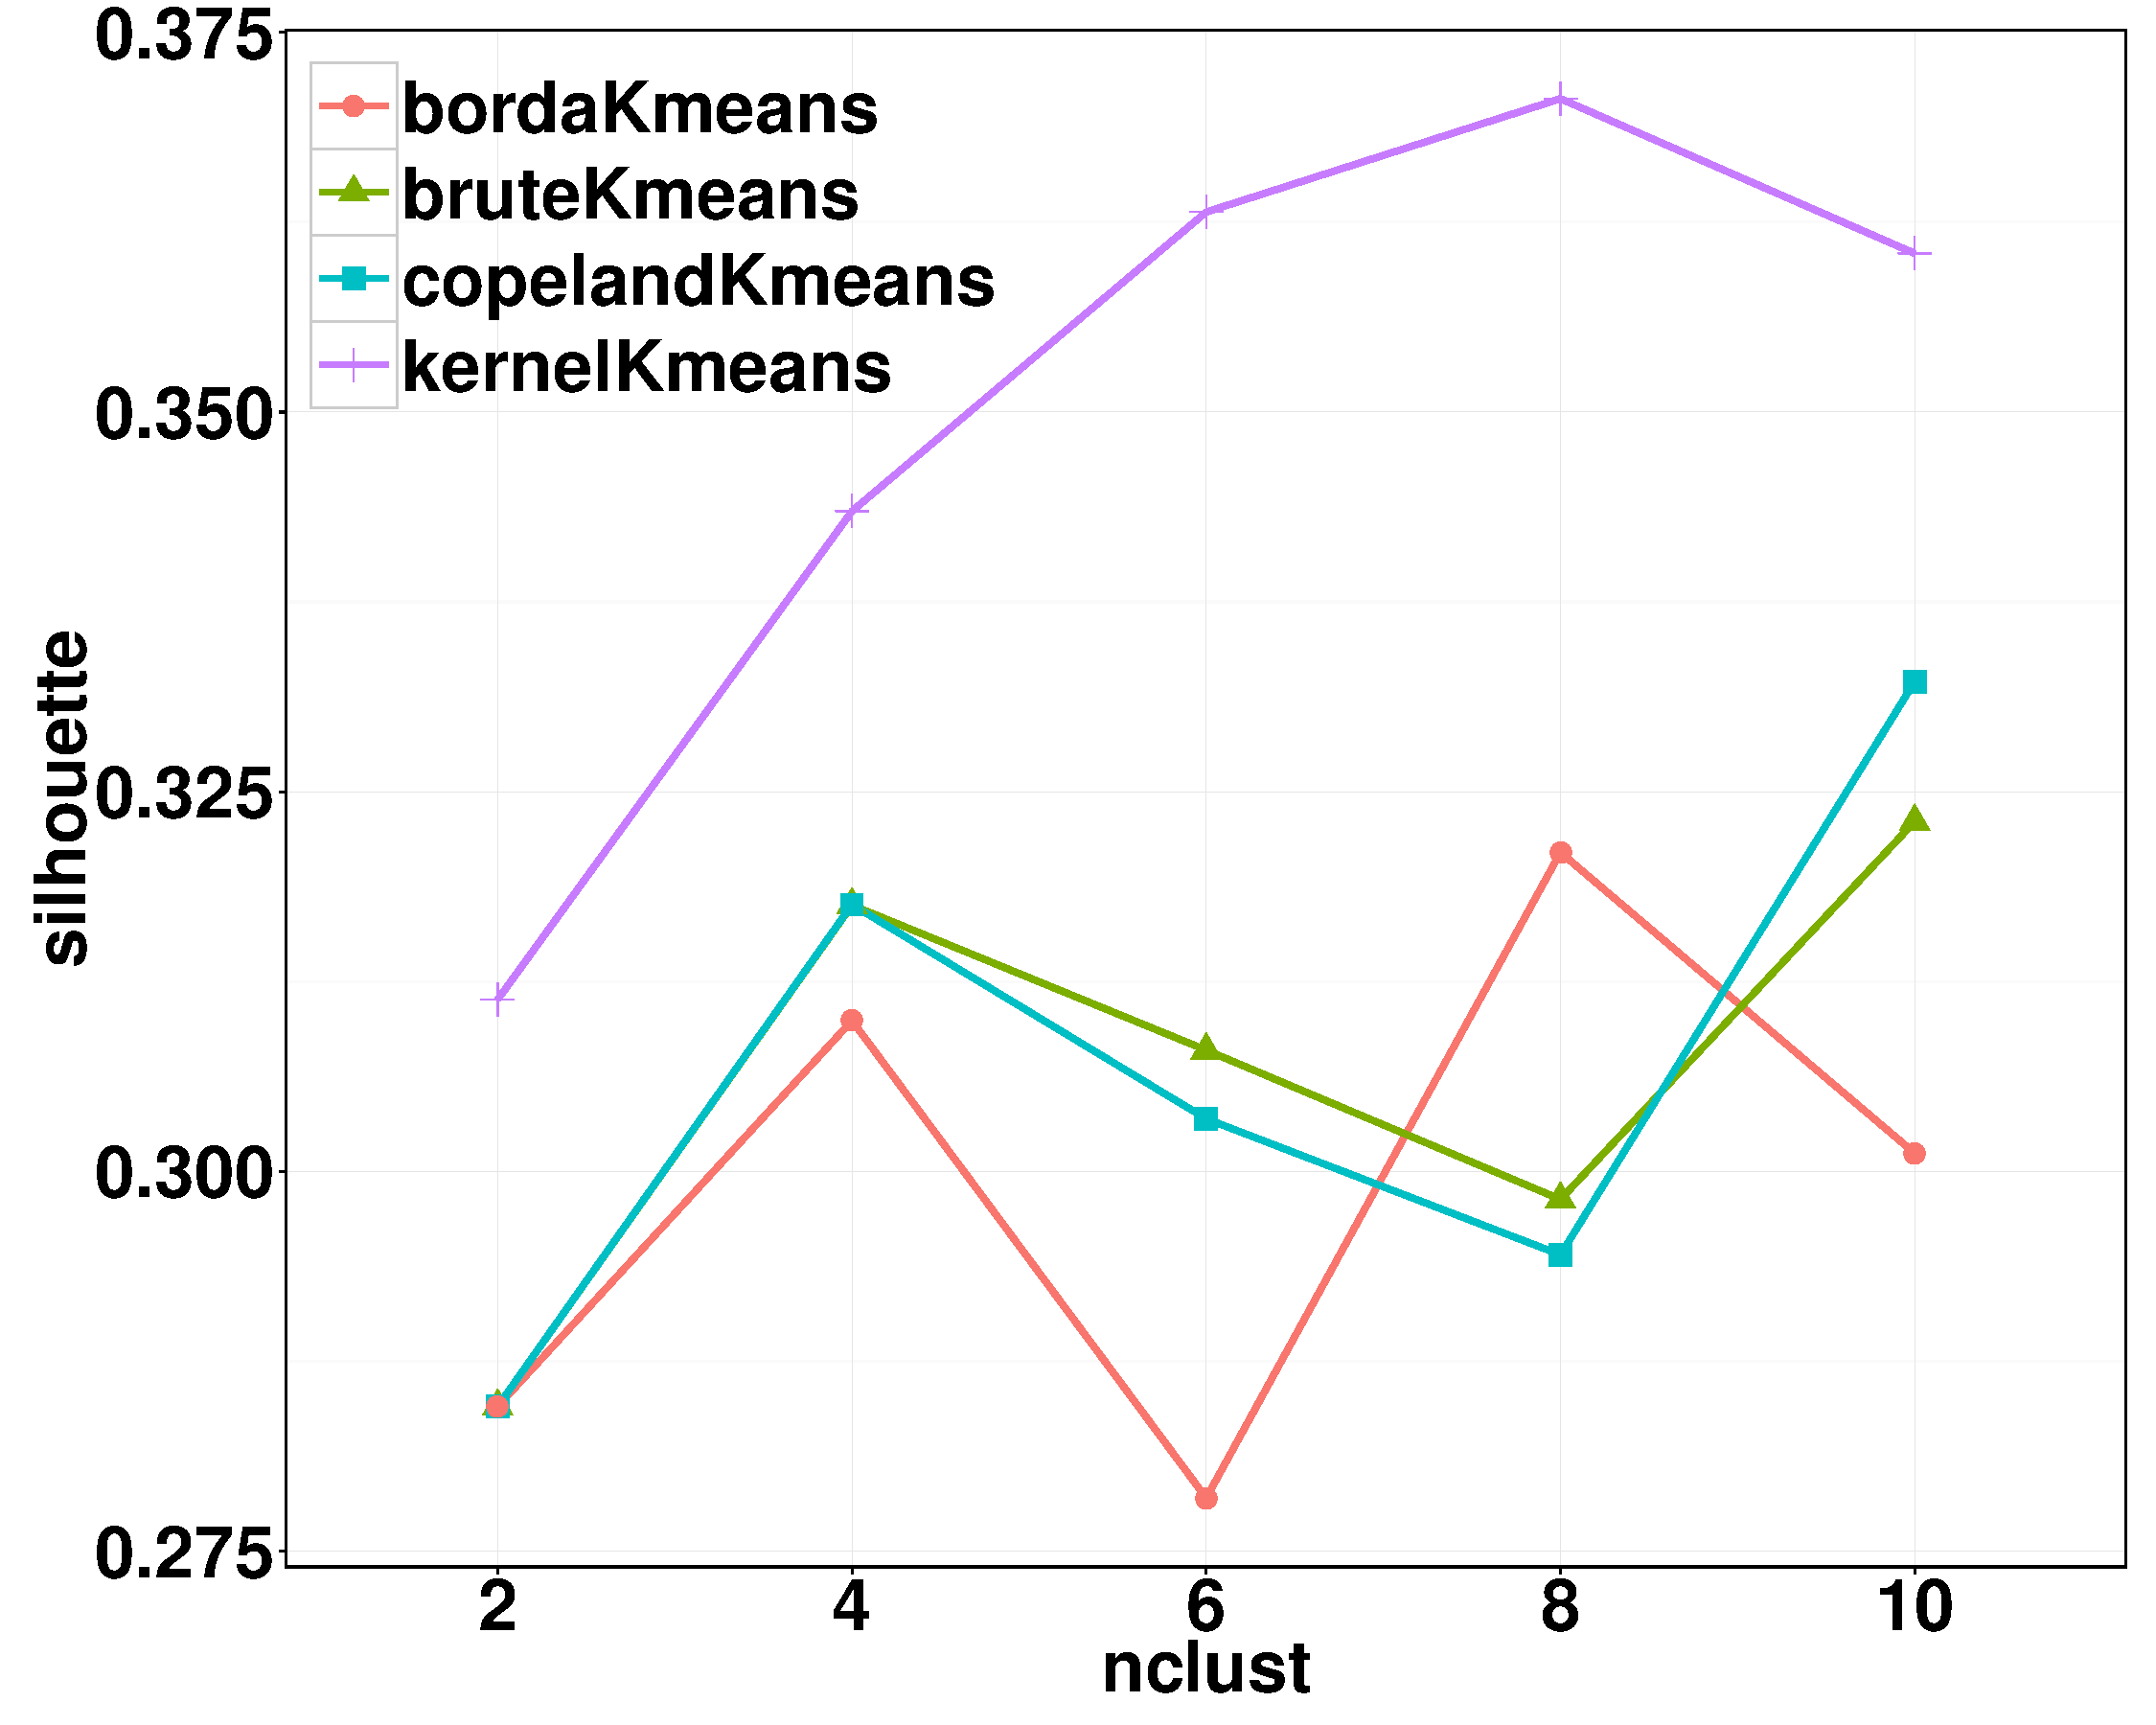
\includegraphics[width=0.6\textwidth]{ch-kendall/cluster_results/kmeans-silhouette}
\caption{Average silhouette scores of $k$-means methods across different number of clusters.}
\label{fig2:kmeans-silhouette}
\end{figure}



Further, good clustering algorithms are supposed be robust to ``perturbation'' in data, in the sense that clusters formed by running an algorithm on bootstrap replicas of the original data should be similar. In other words, if we bootstrap the complete dataset twice and form a clustering with respect to each, the two clustering assignments should be close to each other. Note that in order to measure the similarity of two clustering assignments, we use the (adjusted) Rand index defined by the percentage of instance pairs falling in the same or in different clusters by the two assignments \cite{Hubert1985Comparing}. We now compare the stability performance of the proposed kernel $k$-means and other $k$-means algorithms. Specifically, for each fixed number of clusters, we repeatedly use a bootstrap replica of the dataset to search for centroids returned by running $k$-means algorithms, and partition the original dataset with these identified centroids. The Rand index for two such clustering assignments is computed and the computation is repeated for 100 times accounting for the random process of bootstrapping. Results are shown in Figure \ref{fig2:kmeans-stability}. We observe that, for each fixed number of clusters, kernel $k$-means has higher stability scores than the classic $k$-means algorithms in general. Notably, the discrepancy between kernel $k$-means and the others in terms of their stability performance is even sharper when the number of clusters becomes large. In conclusion, evidence advocates again the use of kernel $k$-means over classic $k$-means algorithms in clustering rank data.


\begin{figure}[!htbp]
\begin{center}
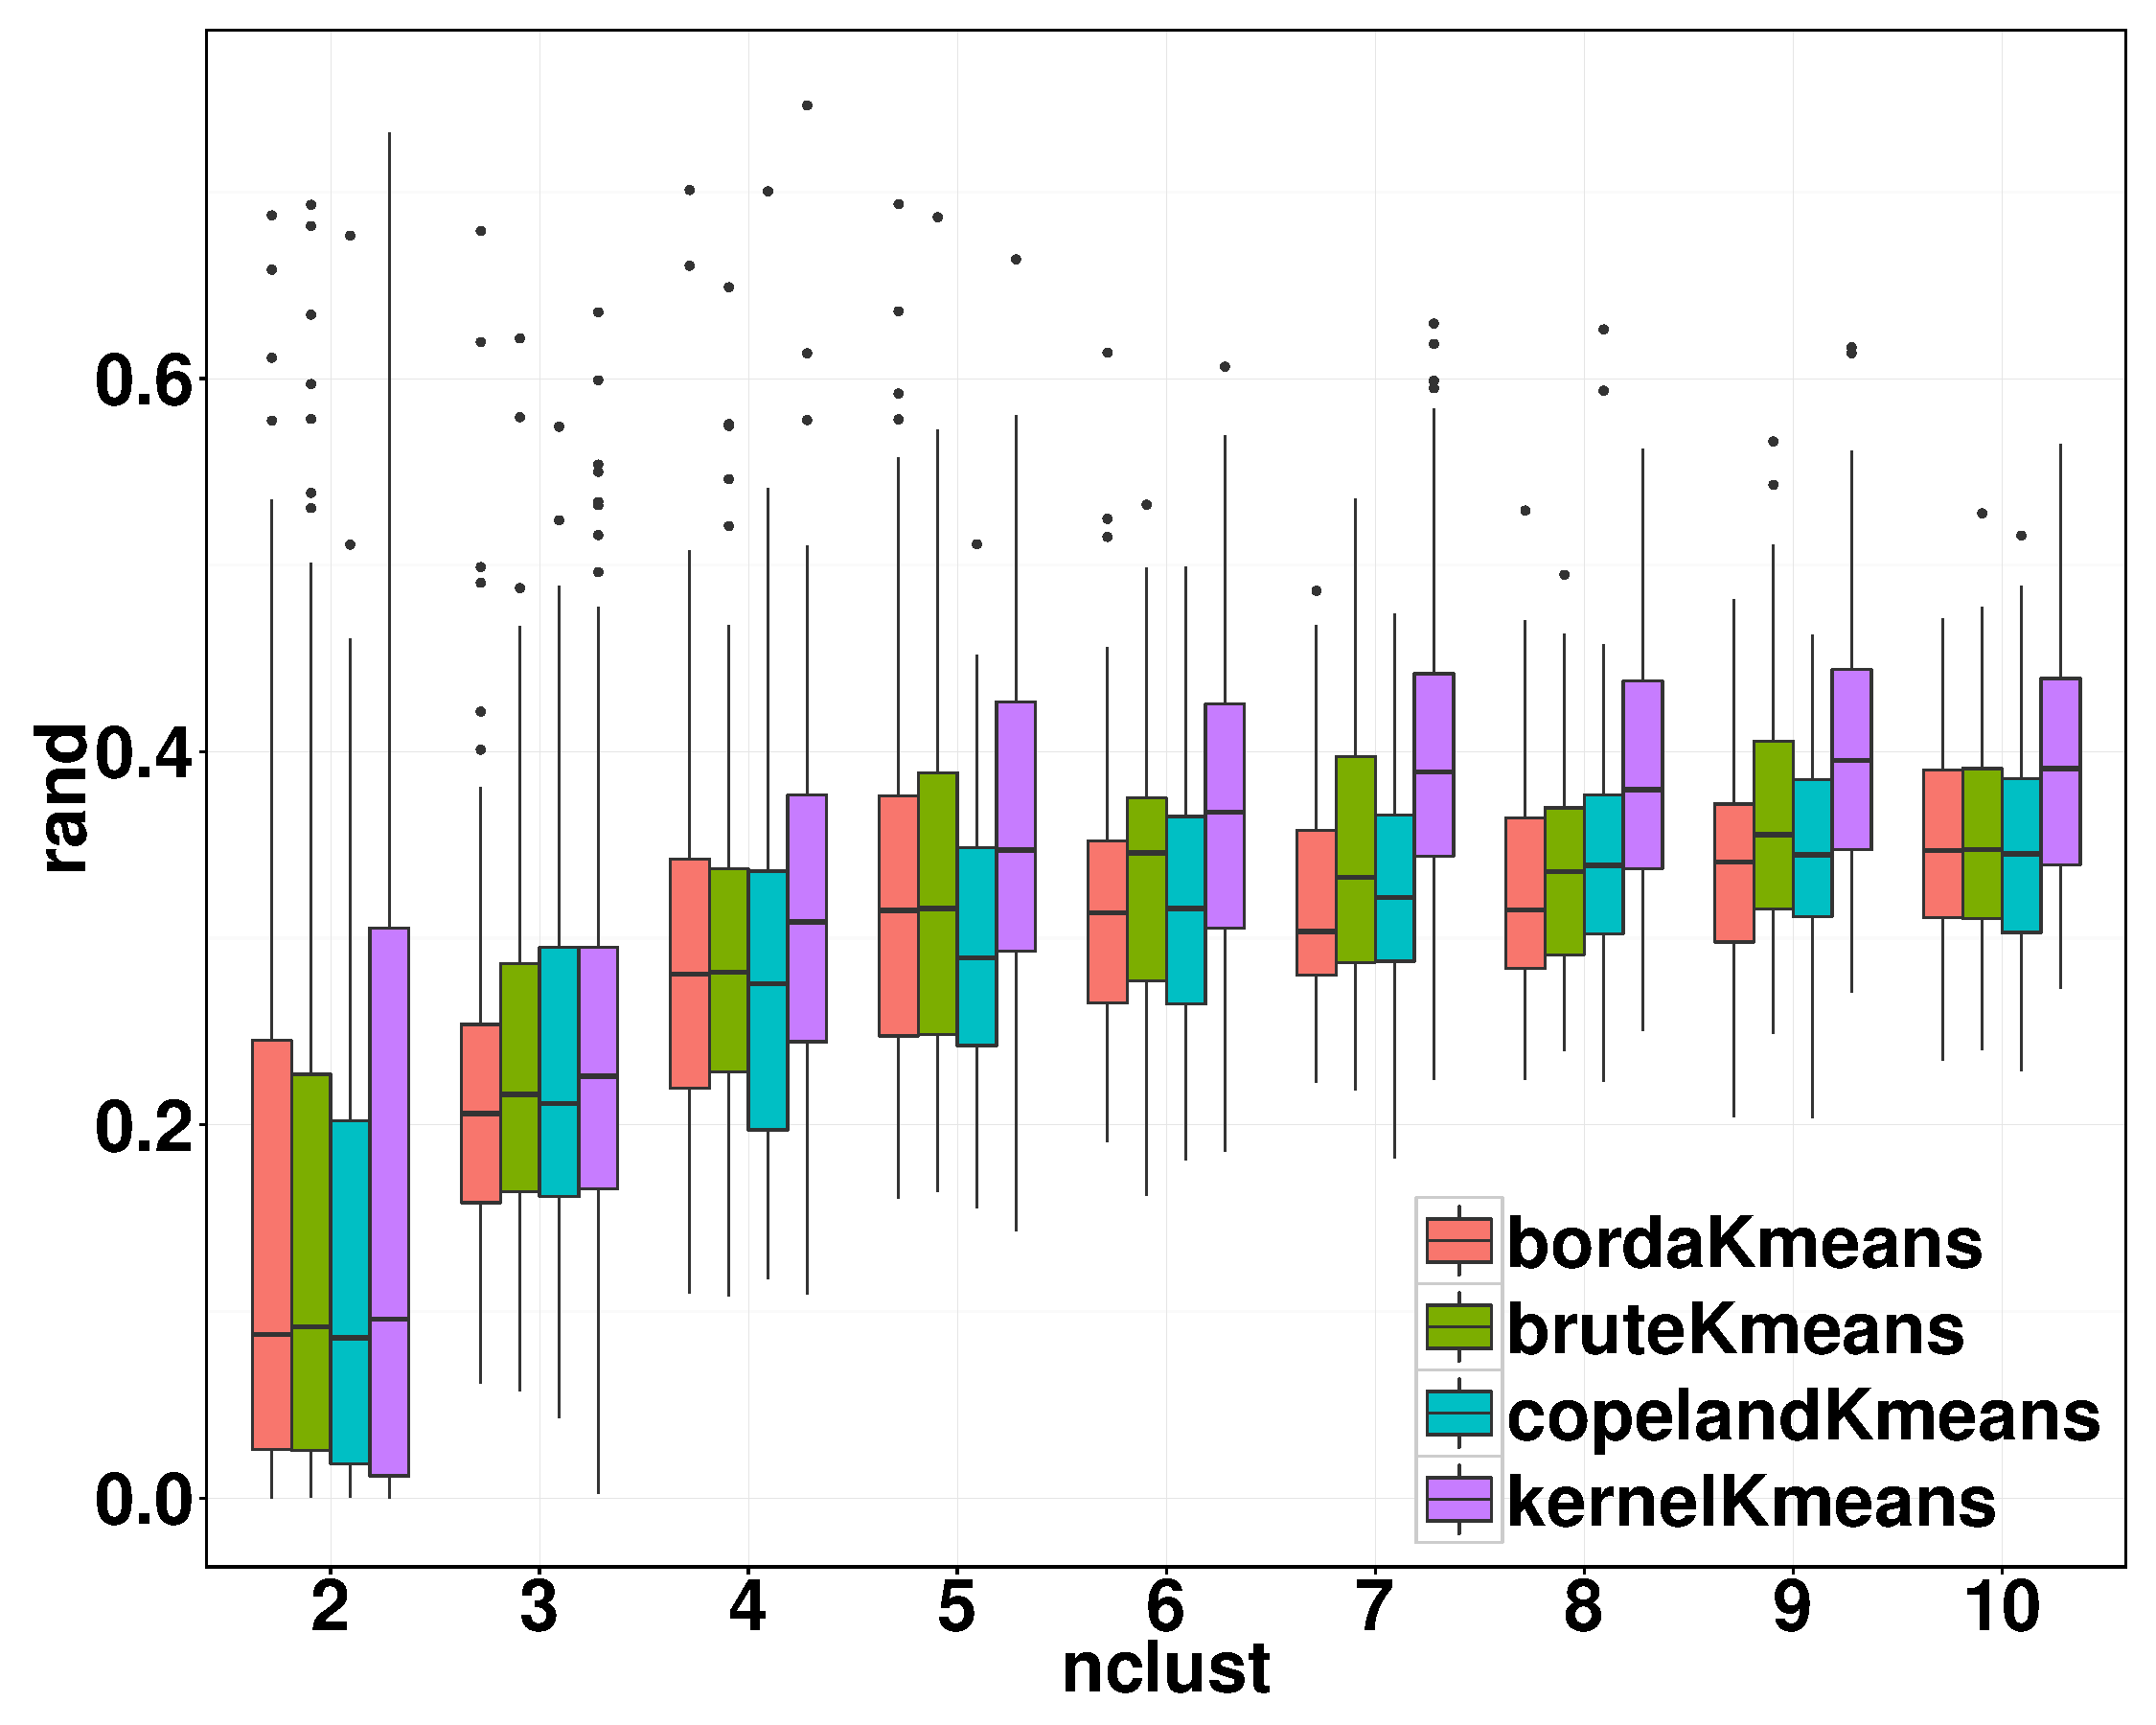
\includegraphics[width=0.6\textwidth]{ch-kendall/cluster_results/kmeans-stability}
\caption{Across different number of clusters, Rand index between clustering assignments by running $k$-means algorithm on bootstrap replicas of the 1980 APA election data. For each fixed number of clusters, the boxplot represents the variance over 100 repeated runs.}
\label{fig2:kmeans-stability}
\end{center}
\end{figure} 


Mixture modeling is then used to fit the data and a partition of the votes is converted from the fitted models forming a clustering result. Baseline models are the Mallows mixture models fitted by the EM algorithm \cite{Murphy2003Mixtures} using three different center-update algorithms at each iteration: brute-force search for Kemeny-optimal ranking, approximate ranking induced by Borda Count and Copeland's method. As proposed in this chapter, we embed the kernel trick in Mallows mixture modeling with two alternatives $g$ \eqref{eq2:kernelmallows} and $g^{\dagger}$ \eqref{eq2:kernelgaussian} in place of $f$ \eqref{eq2:mallowspdf}. In each case, we vary the number of clusters ranging from $2$ to $10$ and the algorithm is repeated $50$ times with randomly initialized configurations for each fixed number of clusters. As shown in Figure \ref{fig2:mallows-silhouette}, modeling a Gaussian mixture to data in the feature space, or equivalently using $g^{\dagger}$ instead of $f$, provides a preferable split of the data into sub-groups with higher average silhouette scores across different number of clusters selected \emph{a priori}.


\begin{figure}[!htbp]
\centering
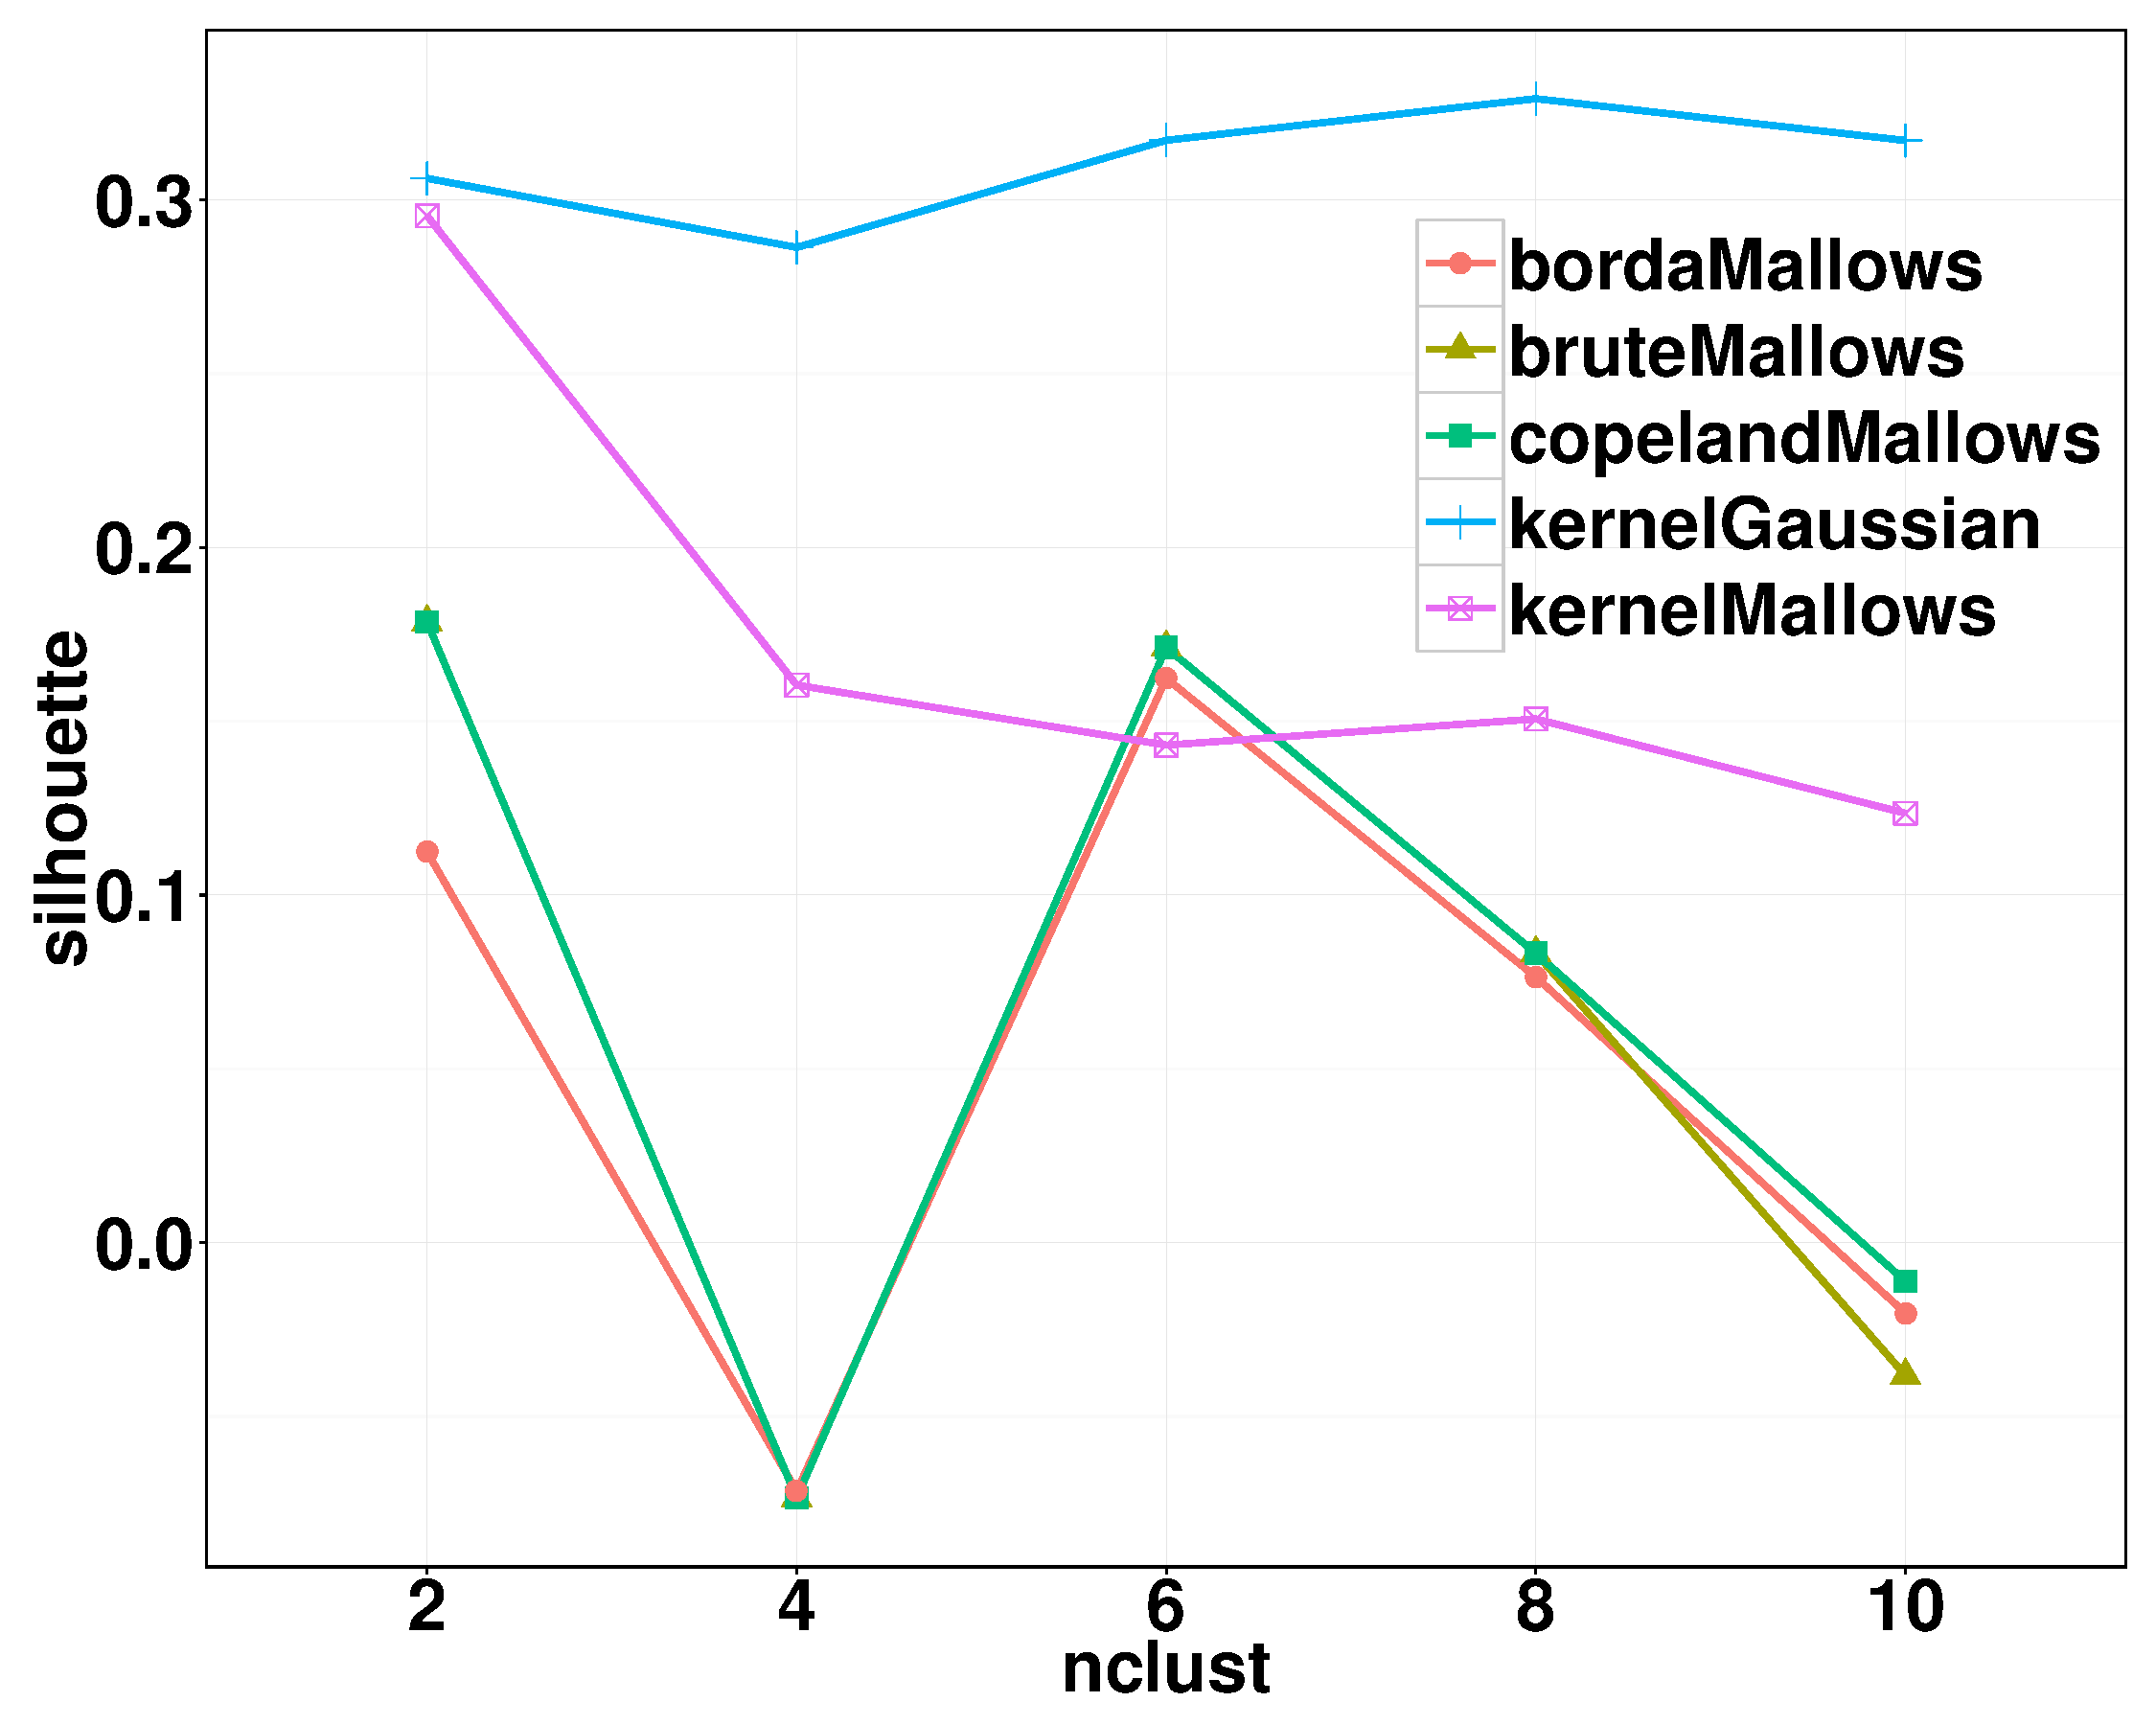
\includegraphics[width=0.6\textwidth]{ch-kendall/cluster_results/mallows-silhouette}
\caption{Average silhouette scores of Mallows mixture modeling methods across different number of clusters.}
\label{fig2:mallows-silhouette}
\end{figure}


\noindent {\bf Clustering ESC voting data.} We finally perform clustering on a dataset of multivariate partial rankings. In the finale of Eurovision Song Contest (ESC), each participating country casts one top-$k$ vote over the finalists who represent their home country. Taken from \cite{Jacques2014Model}, the dataset consists of $34$ multivariate ranking instances, each being a series of $6$ partial votes over top $8$ finalists from 2007 to 2012 respectively.



In comparison with the mixture of Insertion Sorting Rank (ISR) model for clustering multivariate partial rank data proposed by \cite{Jacques2014Model}, we implement the kernel $k$-means algorithm (Algorithm \ref{alg:kernelkmeans}) with the extended Kendall kernel to multivariate rankings \eqref{eq2:multivariate} and equal weights $\mu_j=1/p$ where $p=6$ corresponding to the six contests across years. For each fixed number of clusters, the kernel $k$-means algorithm is repeated $100$ times with randomly initialized configurations while $10$ times for the ISR mixture modeling approach. We vary the number of clusters ranging from $2$ to $6$, and the optimal number is selected to be $2$ for kernel $k$-means with respect to highest average silhouette score while $5$ for the ISR mixture model with respect to highest BIC value. It consumes $2$ hours in total to fit the ISR mixture model in order for clustering while it only takes less than $10$ seconds to form the partition of data with kernel $k$-means. Although it is beyond the scope of this study to further explore the meaningful voting blocs, the colored map of Asia-Europe in terms of clustering results of participating countries to the ESC according to their voting behavior (Figure \ref{fig2:eurovision}, Left) depicts that there exists interesting geographical alliances between countries in the voting data. For example, country-clusters returned by both algorithms present a sign of strong amity within Eastern Europe. Silhouette plots for both algorithms are shown in Figure \ref{fig2:eurovision} (Right). Despite a relatively small number of clusters selected for the kernel $k$-means, the silhouette plot (Figure \ref{fig2:eurovision-kkmeans}, Right) attests that the underlying clusters are well formed. Note that both silhouette plots opt for the same distance used by kernel $k$-means, which may show bias against a clustering scheme based on probabilistic modeling with ISR mixtures. However, the two approaches behave distinctly in identifying subgroups. For example, the ISR mixture model distinguishes Portugal as a singleton among all countries, while interpreting such clustering results remains to be studied. On the other hand, the $k$-means based approach tends to find more evenly distributed subgroups, in the sense that the number of individuals in each subgroup is more consistent. Therefore kernel $k$-means clustering is favored if the study of interest lies in populous behaviors in voting despite of potential outlier individuals. Notably the detection of outliers can be done by other kernel algorithms (Section \ref{sec2:discussion}).

\begin{figure}[!htbp]

\begin{subfigure}{\textwidth}
\centering
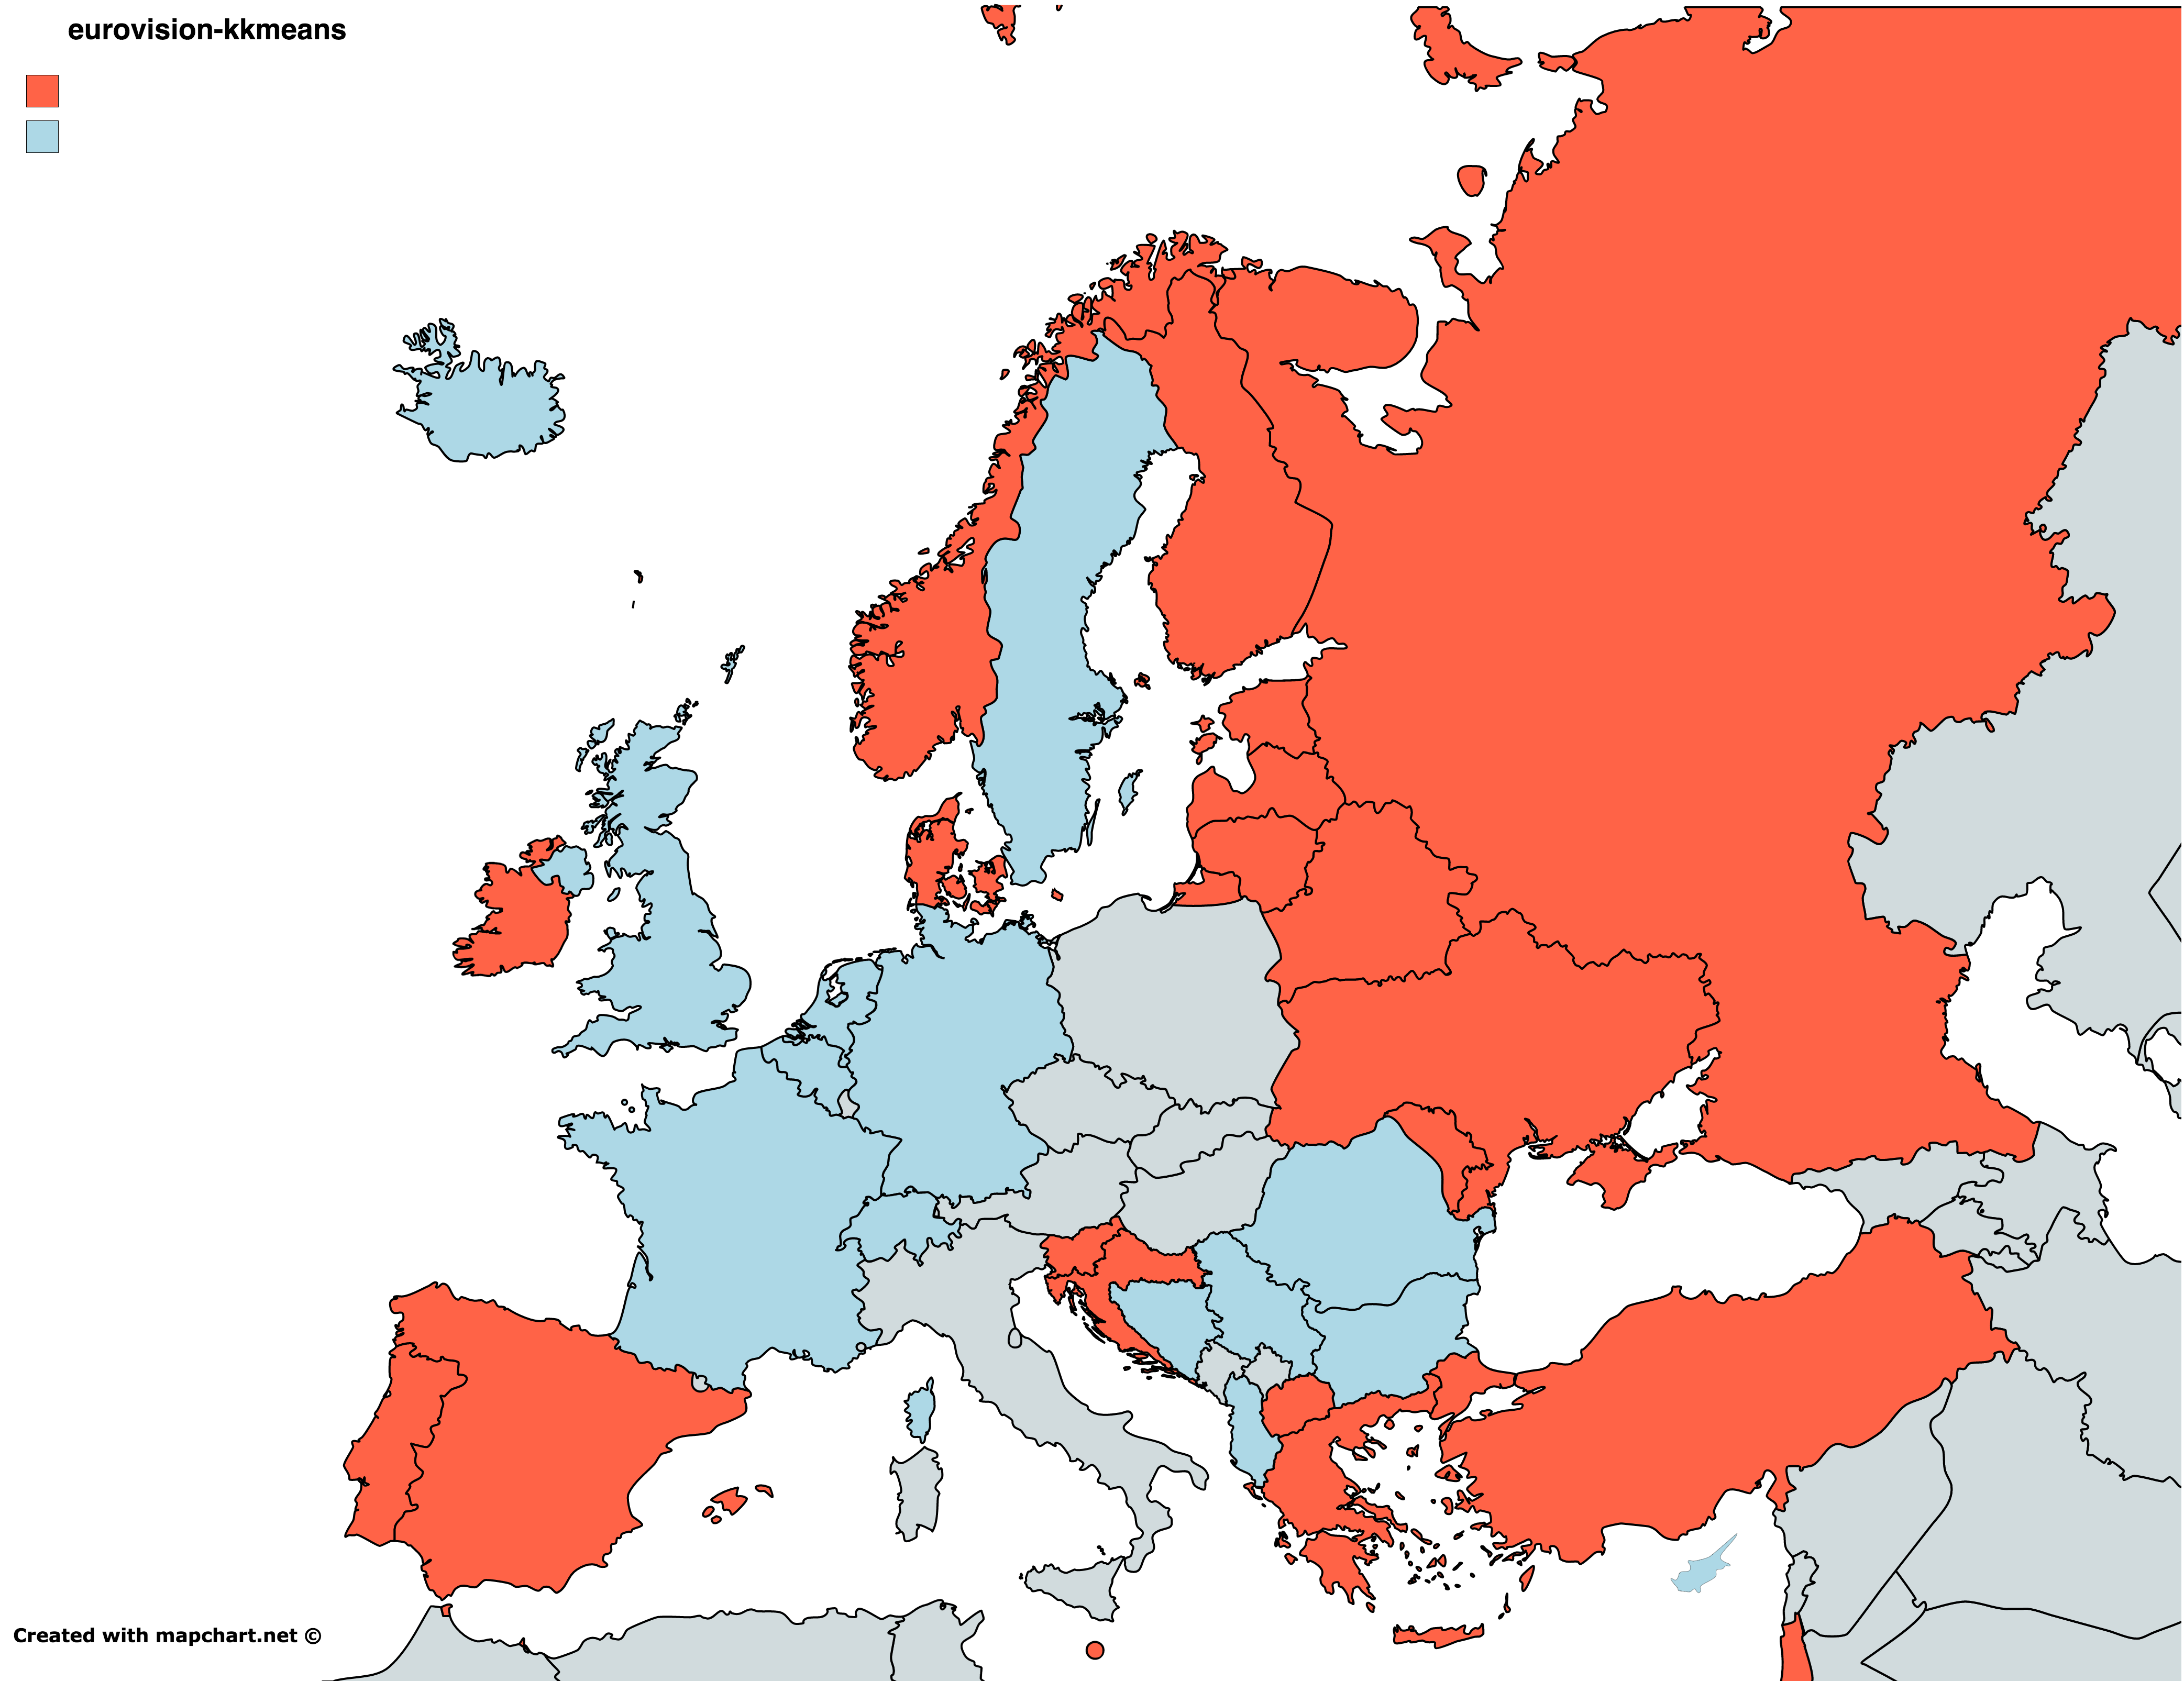
\includegraphics[width=0.45\textwidth]{ch-kendall/cluster_results/eurovision-kkmeans}%
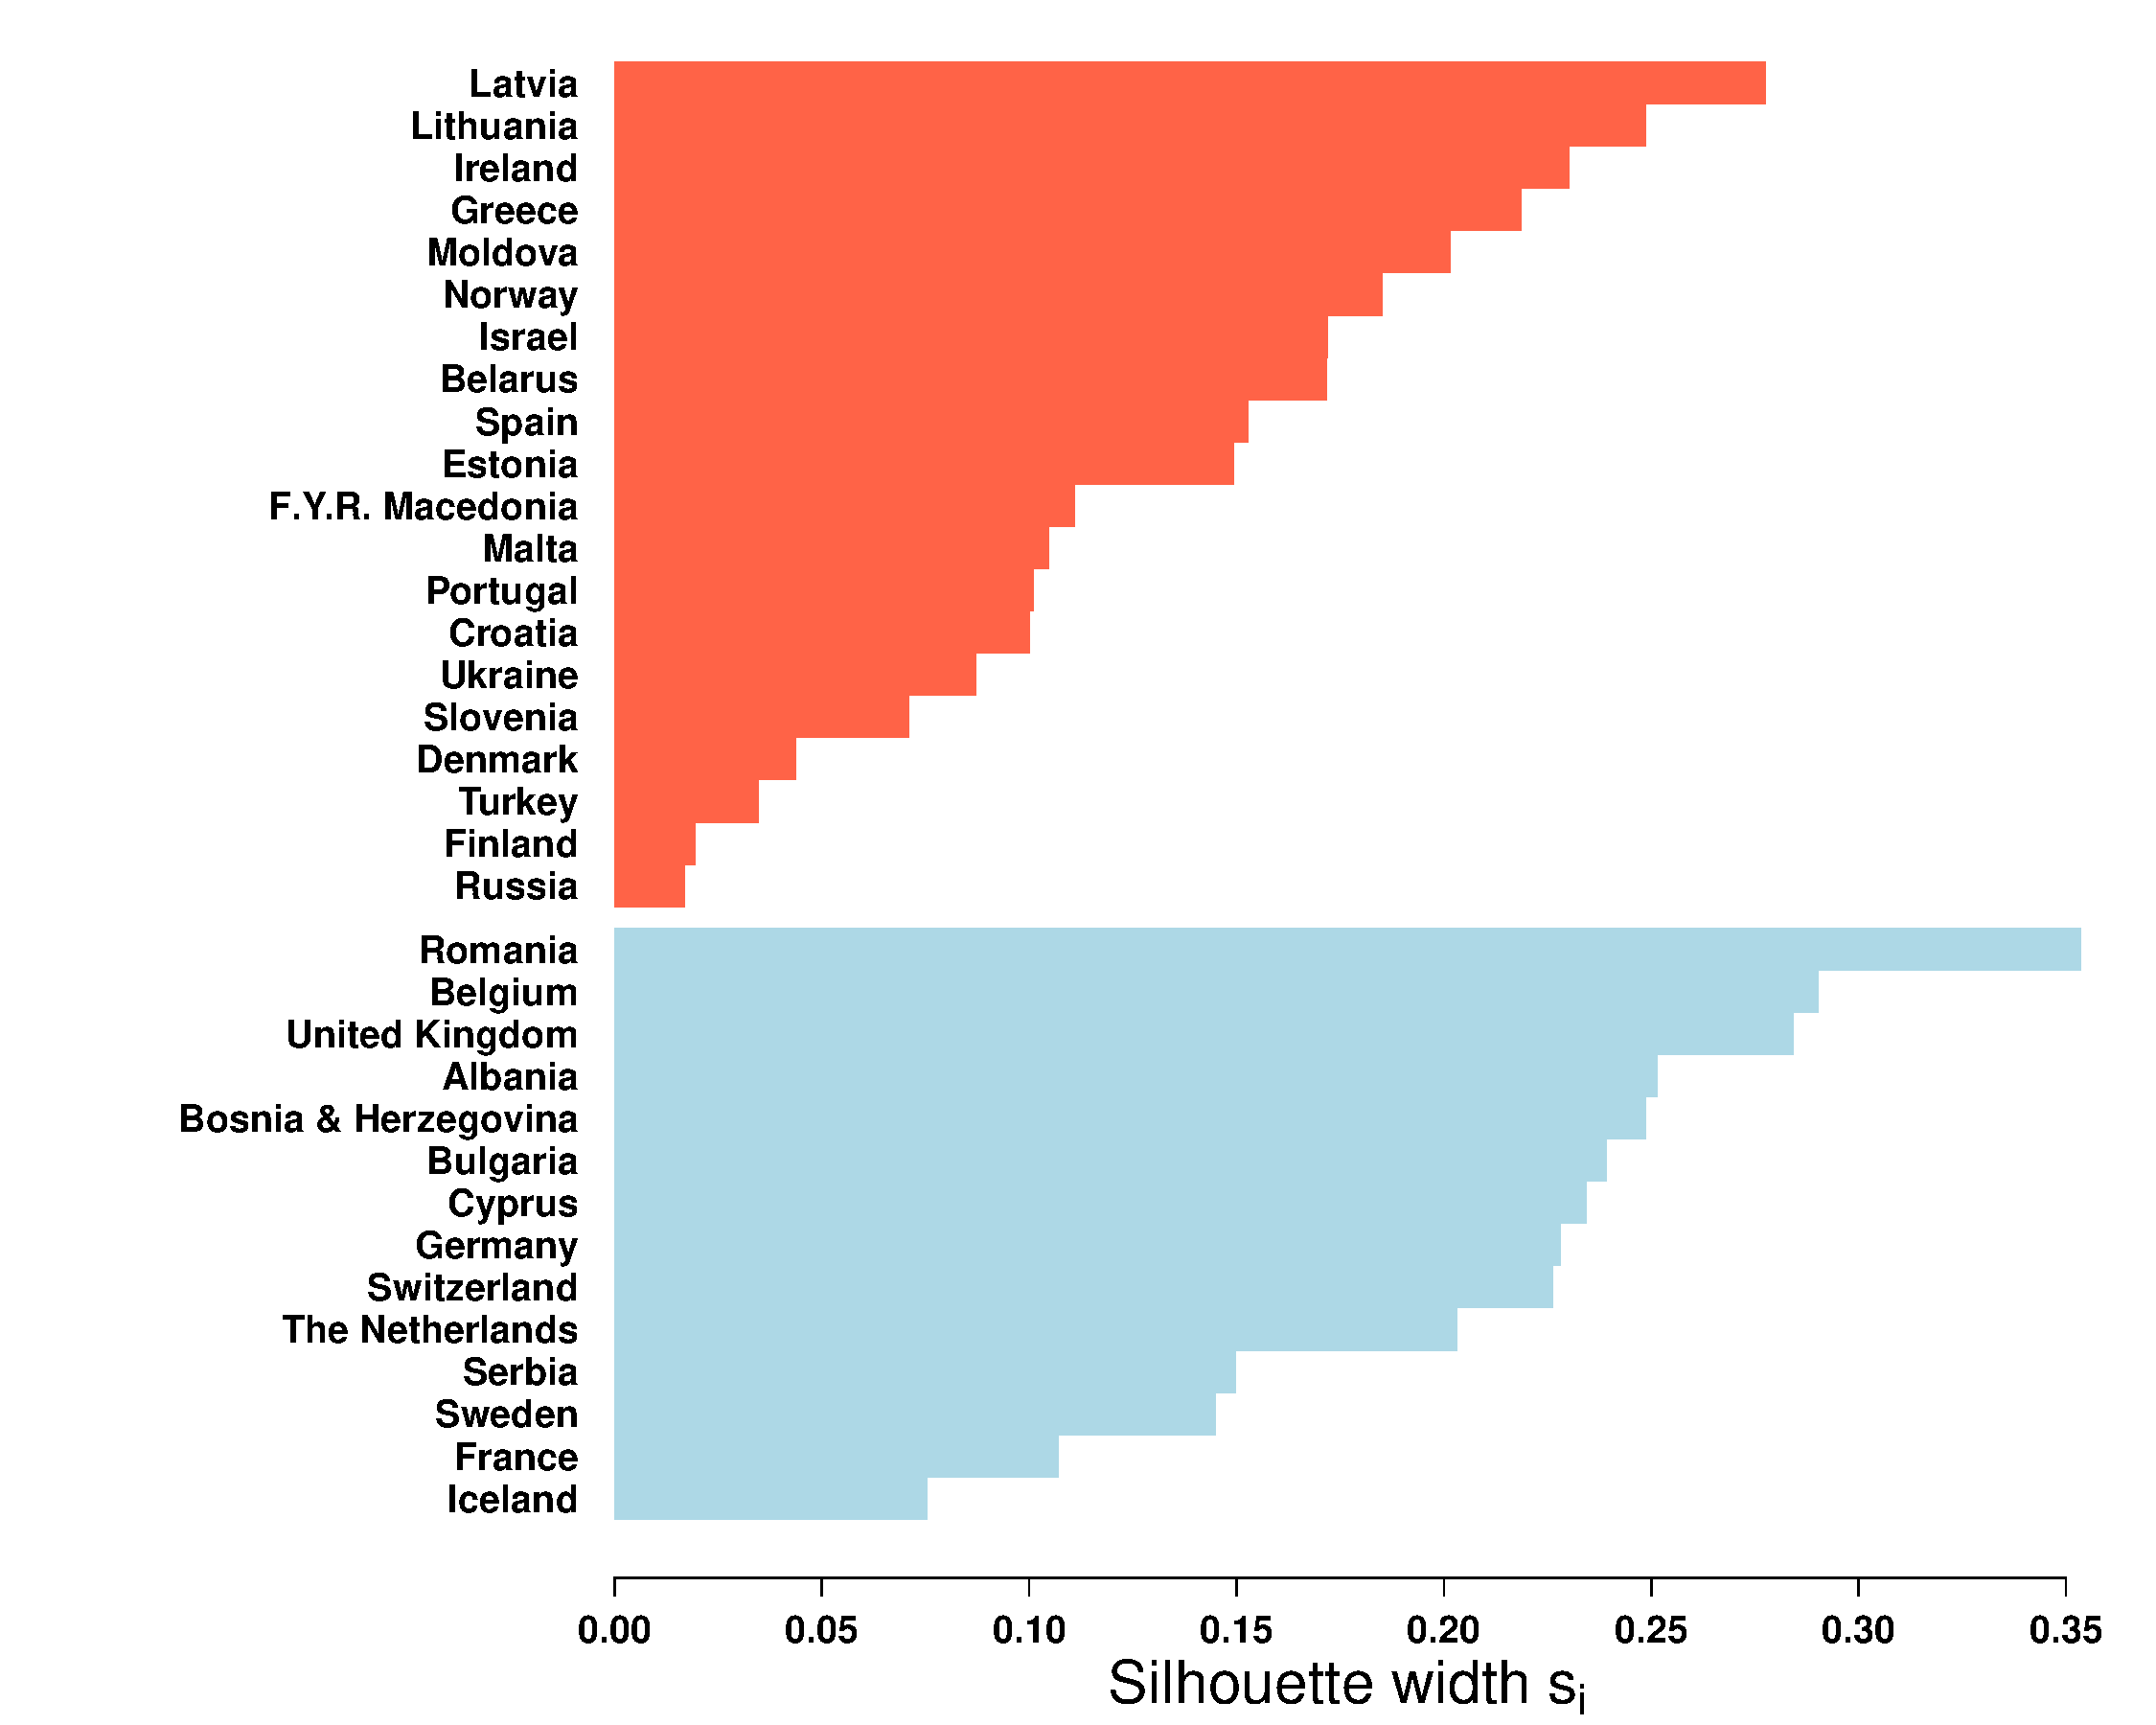
\includegraphics[width=0.45\textwidth]{ch-kendall/cluster_results/eurovision-silhouette-kkmeans}
\caption{Country-clusters returned by kernel $k$-means, where the number of clusters $2$ is selected with respect to highest silhouette score averaged over all countries.}
\label{fig2:eurovision-kkmeans}
\end{subfigure}

\begin{subfigure}{\textwidth}
\centering
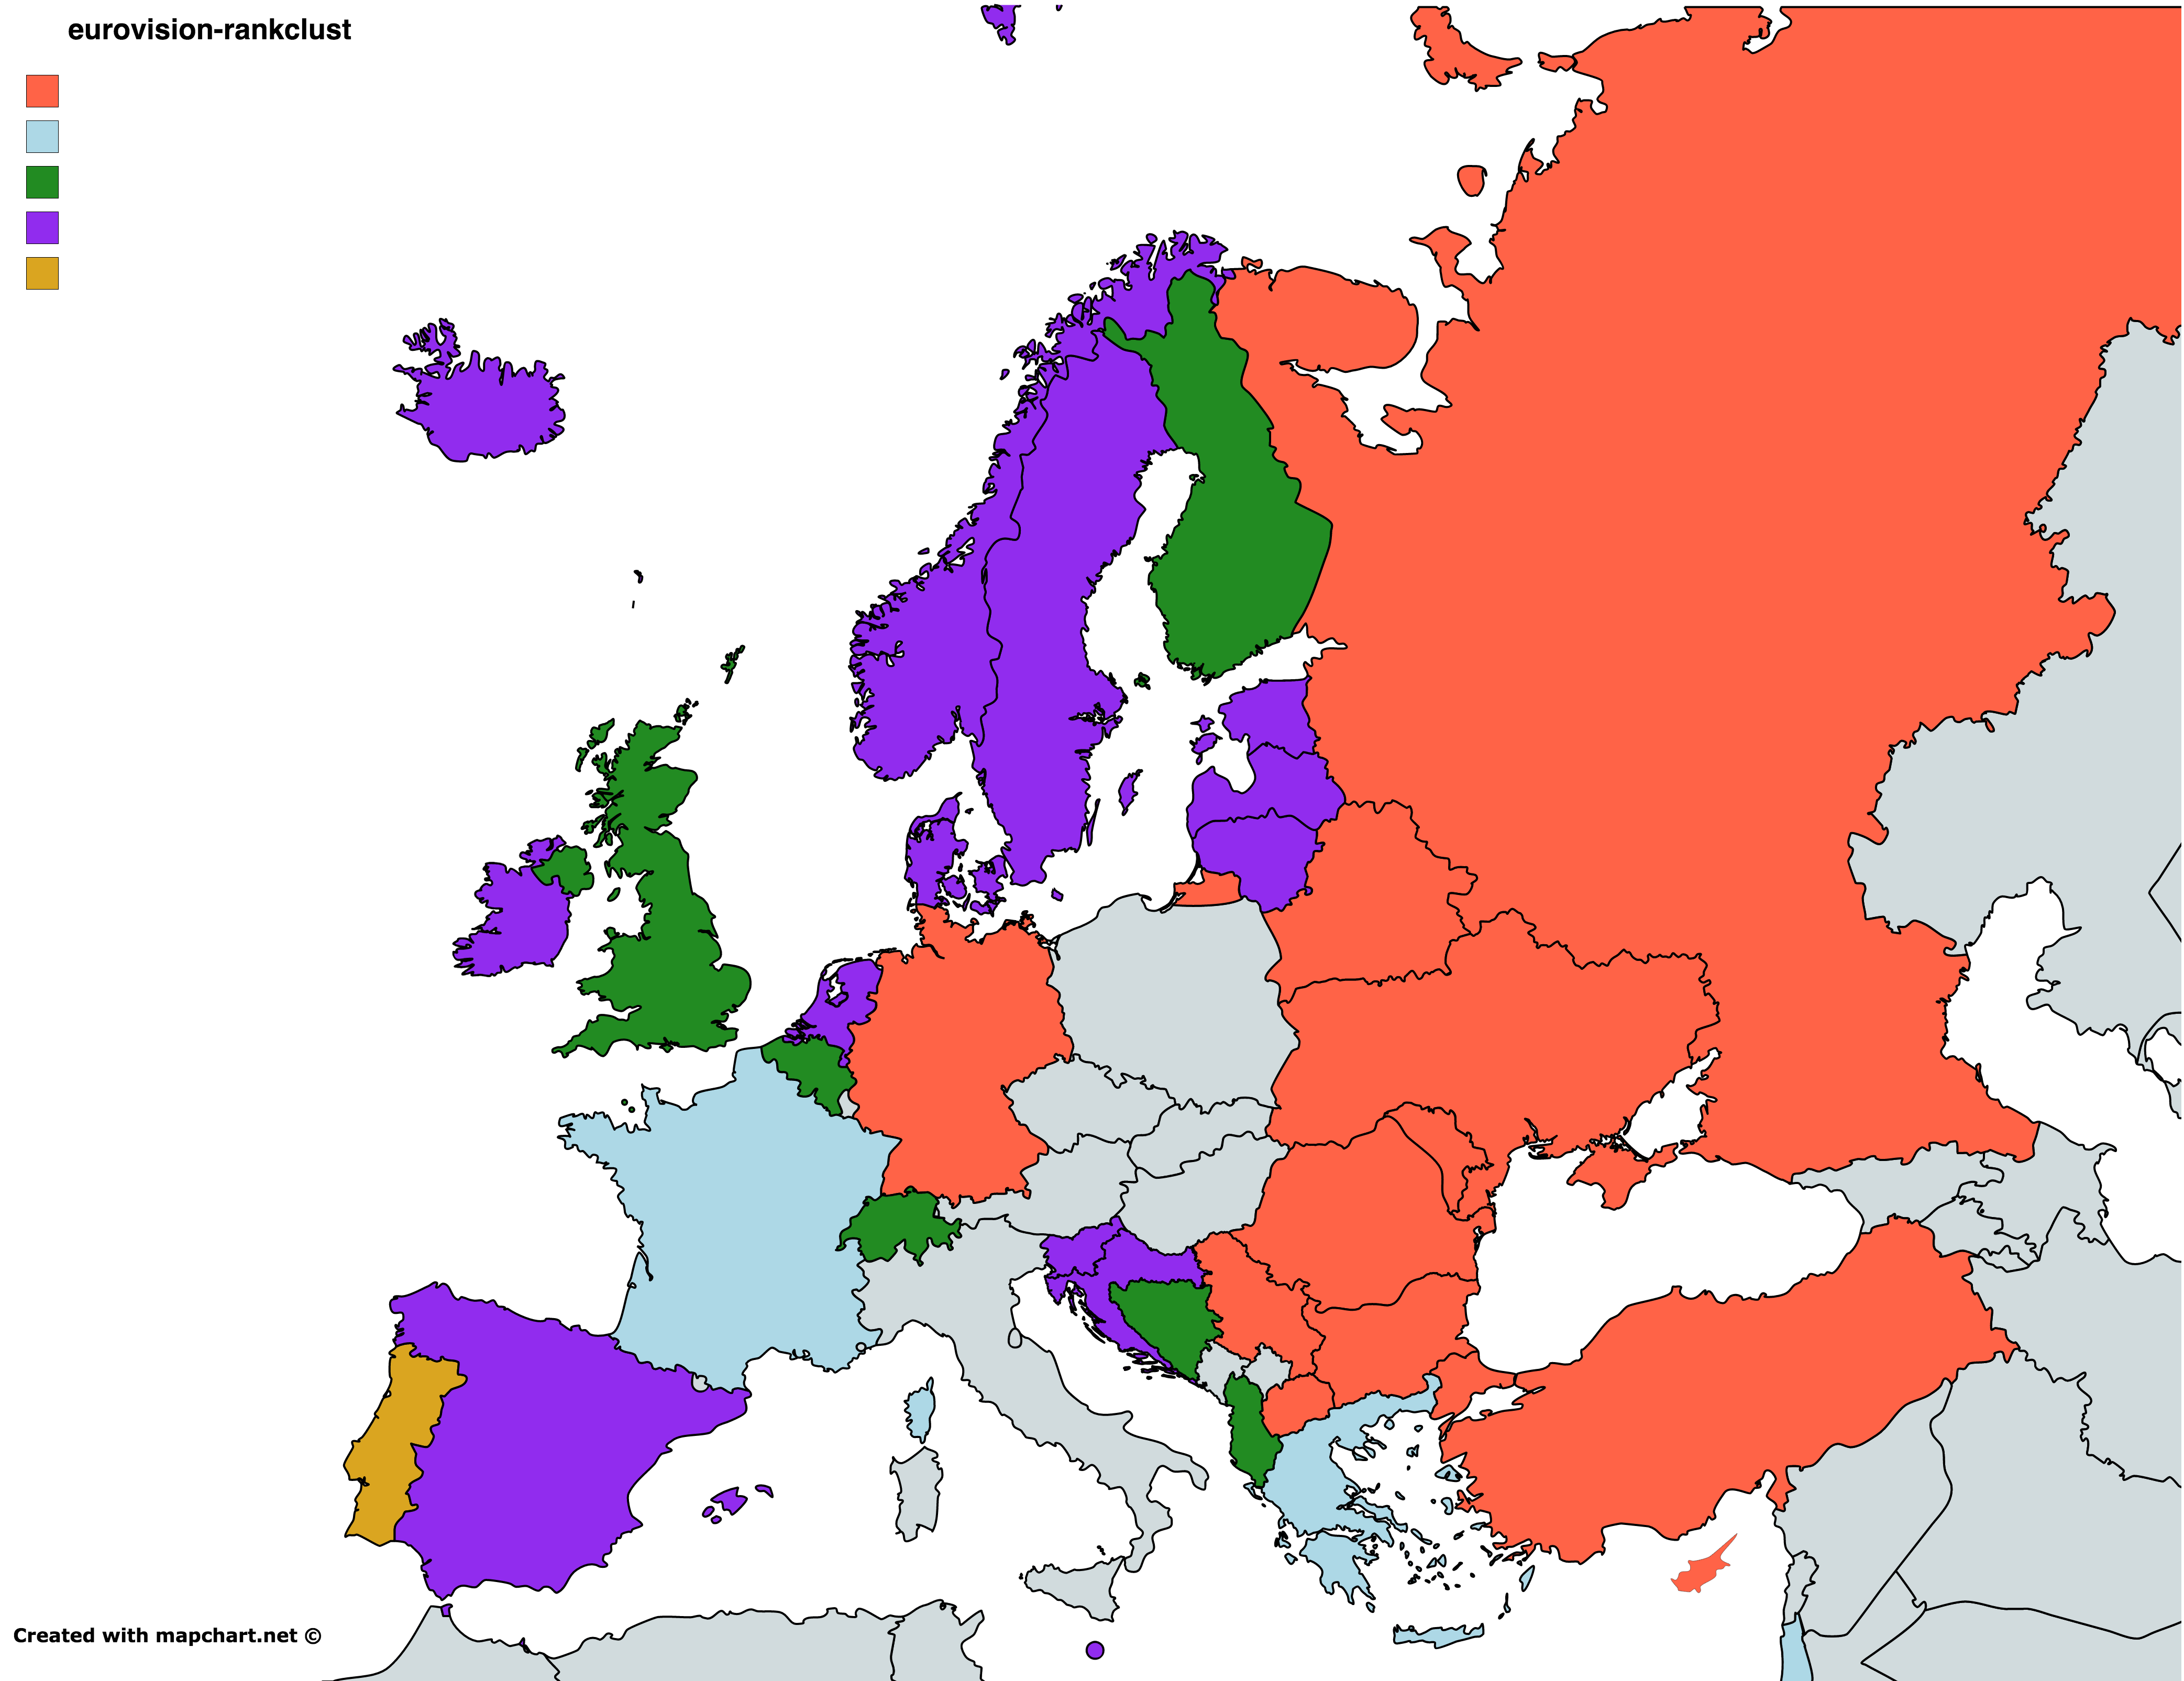
\includegraphics[width=0.45\textwidth]{ch-kendall/cluster_results/eurovision-rankclust}%
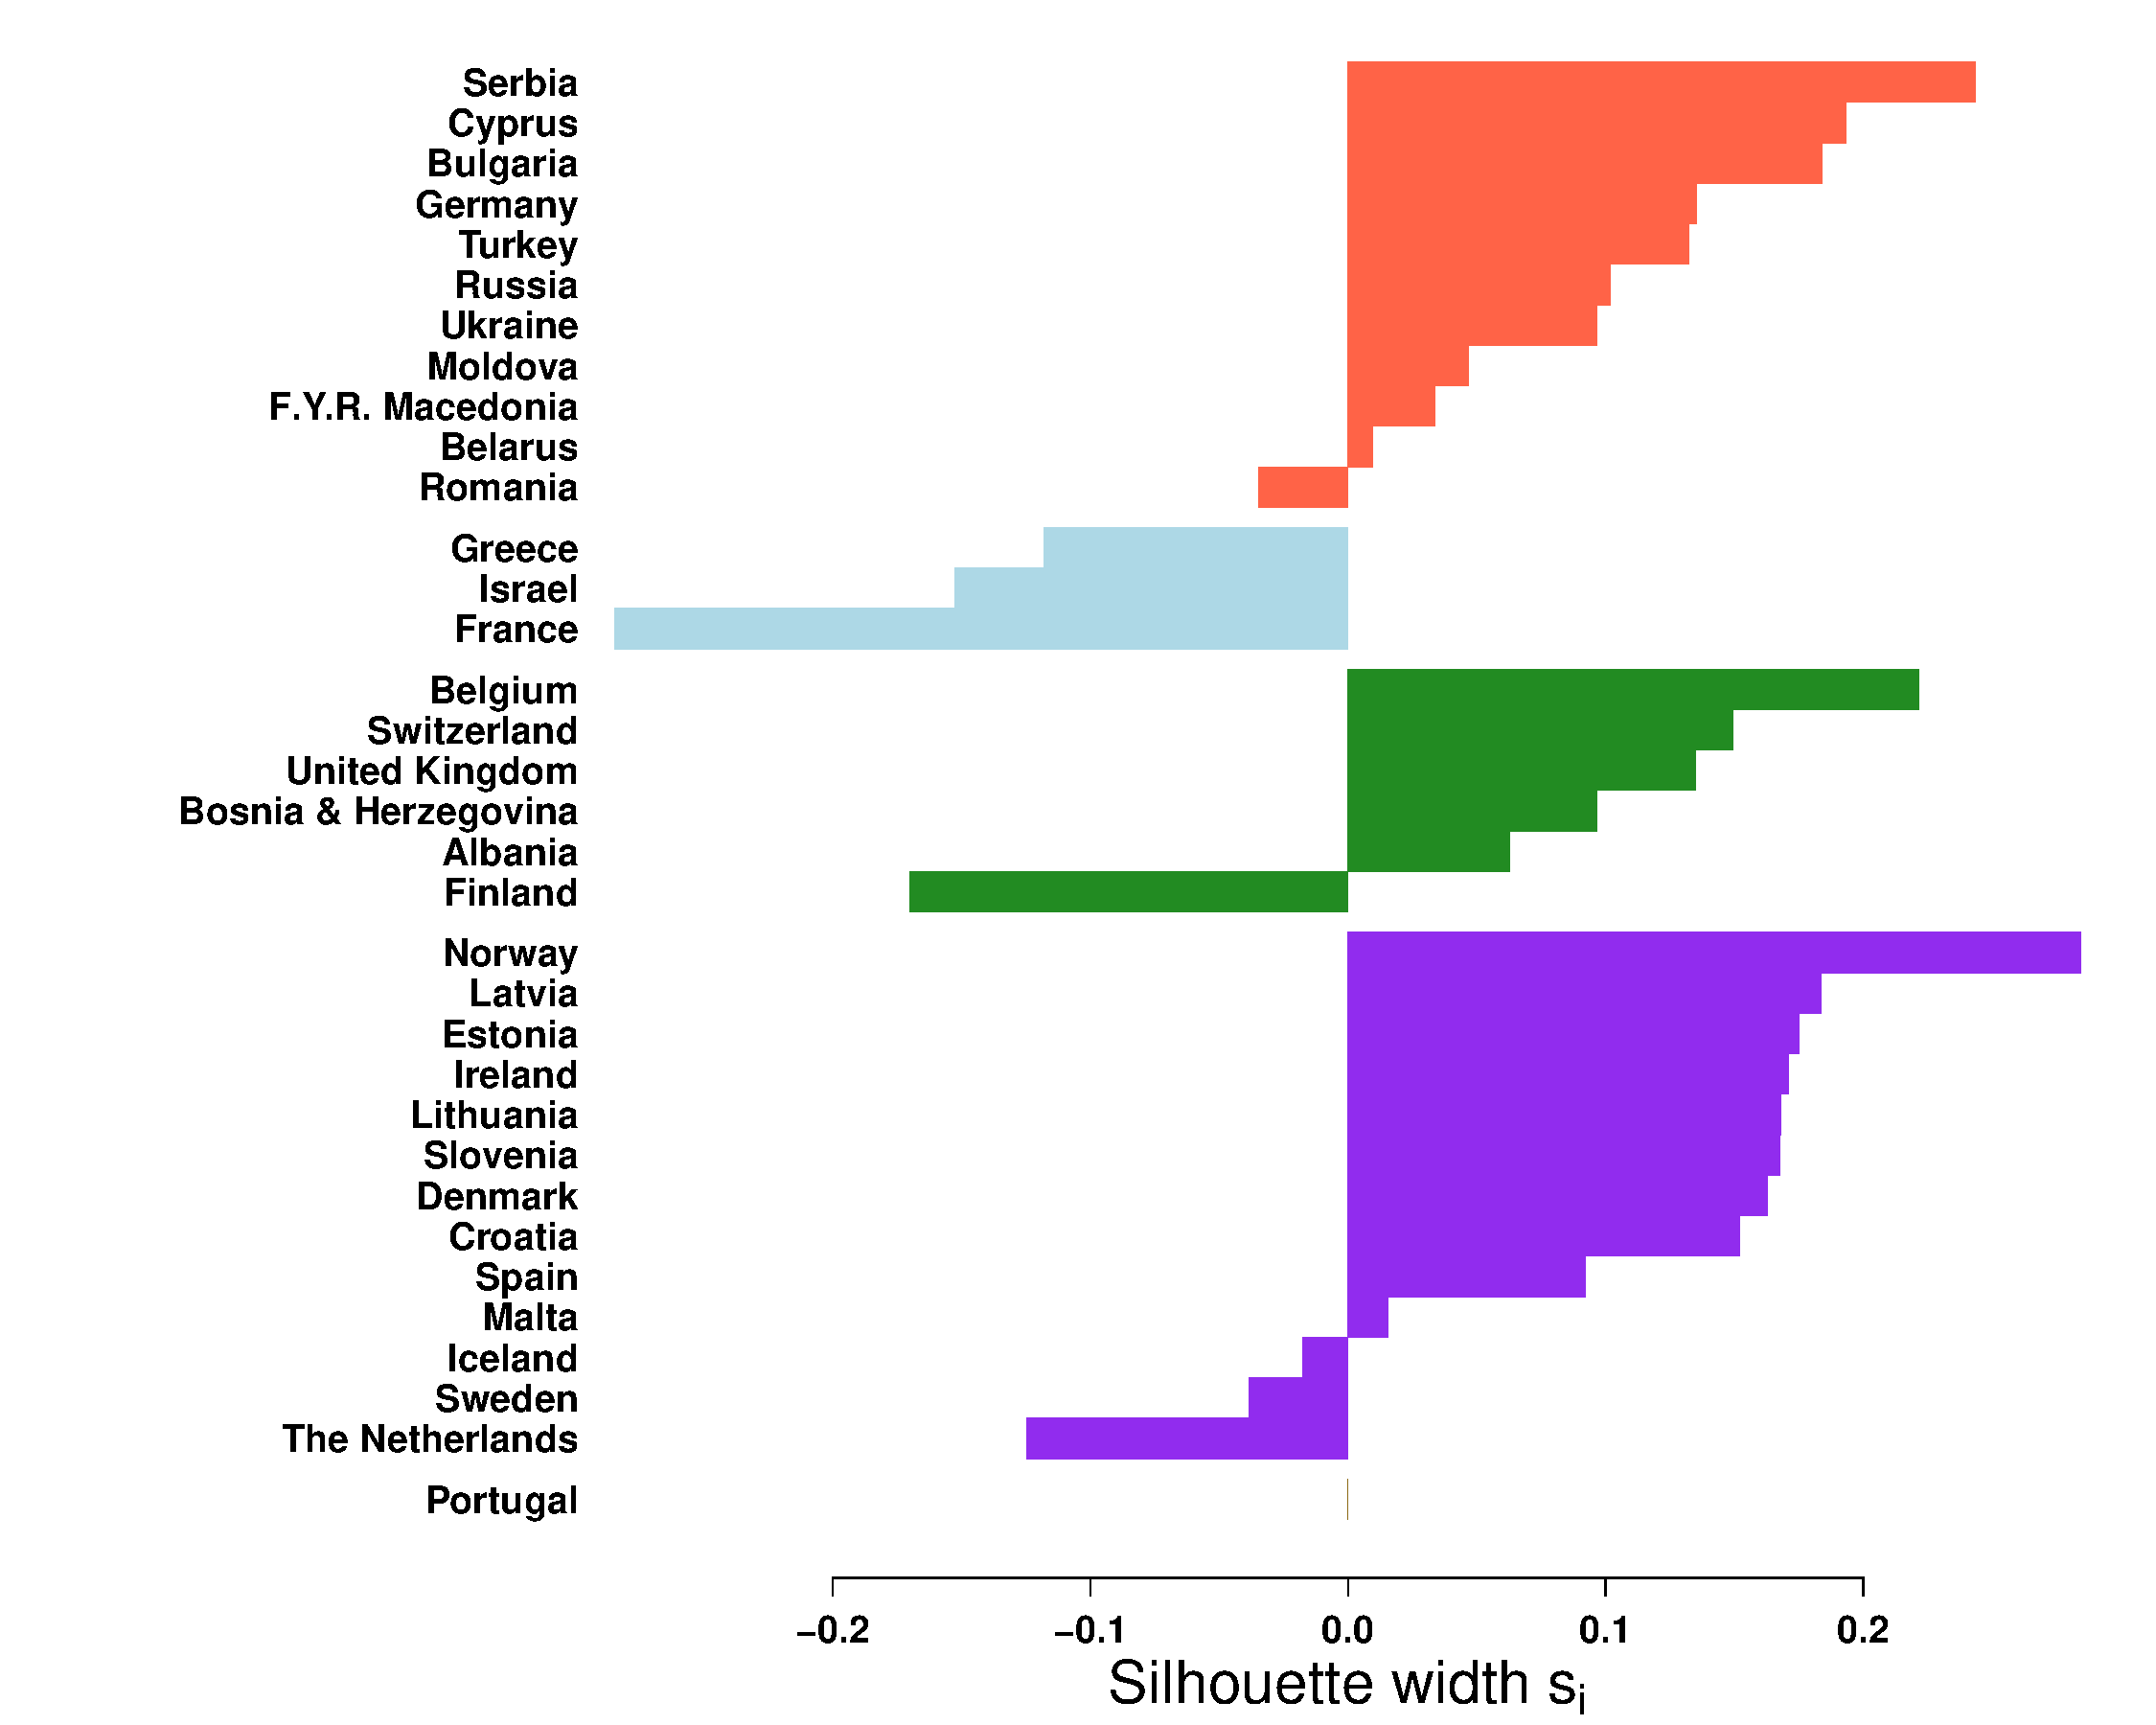
\includegraphics[width=0.45\textwidth]{ch-kendall/cluster_results/eurovision-silhouette-rankclust}
\caption{Country-clusters returned by ISR mixture modeling, where the number of clusters $5$ (including in particular ``Portugal'' as a singleton) is selected with respect to highest fitted BIC value.}
\label{fig2:eurovision-rankclust}
\end{subfigure}

\caption{Clustering results of participating countries to the ESC according to their voting behavior illustrated by geographic map and silhouette plot.}
\label{fig2:eurovision}
\end{figure}



\section{Application: Supervised Classification of Biomedical Data}
\label{sec2:classification}



In this section we illustrate the relevance of supervised classification of rank data with an SVM using the Kendall kernel, when the ranking are derived from a high-dimensional real-valued vector. More precisely, we investigate the performance of classifying high-dimensional biomedical data, motivated by previous work demonstrating the relevance of replacing numerical features by pairwise comparisons in this context \cite{Geman2004Classifying,Tan2005Simple,Xu2005Robust,Lin2009ordering}. 



For that purpose, we collected 10 datasets related to human cancer research publicly available online \cite{Li2003Mean,Schroeder2011breastCancerTRANSBIG,Shi2011Top}, as summarized in Table \ref{tab2:exprdataset}. The features are proteomic spectra relative intensities for the \emph{Ovarian Cancer} dataset and gene expression levels for all the others. The contrasting classes are typically ``Non-relapse v.s. Relapse'' in terms of cancer prognosis, or ``Normal v.s. Tumor'' in terms of cancer identification. The datasets have no missing values, except the \emph{Breast Cancer 1} dataset for which we performed additional preprocessing to remove missing values as follows: first we removed two samples (both labeled ``relapse'') from the training set that have around 10\% and 45\% of missing gene values; next we discarded any gene whose value was missing in at least one sample, amounting to a total of 3.5\% of all genes.


\begin{table}[!htbp]
\caption{Summary of biomedial datasets.}
\label{tab2:exprdataset}
\begin{center}
\begin{scriptsize}
\begin{tabular}{ccccc}
\hline
Dataset & No. of features & \multicolumn{2}{c}{No. of samples (training/test)} & Reference \\
& & $C_1$ & $C_2$ & \\
\hline
Breast Cancer 1 & 23624 & 44/7 (Non-relapse) & 32/12 (Relapse) & \cite{Veer2002Gene} \\
%\hline
Breast Cancer 2 & 22283 & 142 (Non-relapse) & 56 (Relapse) & \cite{Desmedt2007Strong} \\
%\hline
Breast Cancer 3 & 22283 & 71 (Poor Prognosis) & 138 (Good Prognosis) & \cite{Wang2005HykGene} \\
%\hline
Colon Tumor & 2000 & 40 (Tumor) & 22 (Normal) & \cite{Alon1999Broad} \\
%\hline
Lung Adenocarcinoma 1 & 7129 & 24 (Poor Prognosis) & 62 (Good Prognosis) & \cite{Beer2002Gene} \\
%\hline
Lung Cancer 2 & 12533 & 16/134 (ADCA) & 16/15 (MPM) & \cite{Gordon2002Translation} \\
%\hline
Medulloblastoma & 7129 & 39 (Failure) & 21 (Survivor) & \cite{Pomeroy2002Prediction} \\
%\hline
Ovarian Cancer & 15154 & 162 (Cancer) & 91 (Normal) & \cite{Petricoin2002Use} \\
%\hline
Prostate Cancer 1 & 12600 & 50/9 (Normal) & 52/25 (Tumor) & \cite{Singh2002Gene} \\
%\hline
Prostate Cancer 2 & 12600 & 13 (Non-relapse) & 8 (Relapse) & \cite{Singh2002Gene} \\
\hline
\end{tabular}
\end{scriptsize}
\end{center}
\end{table}



We compare the Kendall kernel to three standard kernels, namely linear kernel, homogeneous 2nd-order polynomial kernel and Gaussian RBF kernel with bandwidth set with ``median trick'', using SVM (with regularization parameter $C$) and Kernel Fisher Discriminant (KFD, without tuning parameter) as classifiers. In addition, we include in the benchmark classifiers based on Top Scoring Pairs (TSP) \cite{Geman2004Classifying}, namely (1-)TSP, $k$-TSP \cite{Tan2005Simple}\footnote{While the original $k$-TSP algorithm selects only top $k$ \textit{disjoint} pairs with the constraint that $k$ is \textit{less than} 10, we do not restrict ourselves to any of these two conditions since we consider $k$-TSP in this study essentially a feature pair scoring algorithm.} and APMV (all-pairs majority votes, i.e. ${n \choose 2}$-TSP). Finally we also test SVM with various kernels using as input only top features selected by TSP \cite{Shi2011Top}.

In all experiments, each kernel is centered (on the training set) and scaled to unit norm in the feature space. For KFD-based models, we add $10^{-3}$ on the diagonal of the centered and scaled kernel matrix, as suggested by \cite{Mika1999Fisher}. The Kendall kernel we use in practice is a soft version to \eqref{eq2:kdtALL} in the sense that the extremes $\pm 1$ can still be attained in the presence of ties, specifically we use
\begin{equation*}
	K_{\tau}(\mathbf{x},\mathbf{x}') = \frac{n_c(\mathbf{x},\mathbf{x}')-n_d(\mathbf{x},\mathbf{x}')}{\sqrt{(n_0-n_1)(n_0-n_2)}} \,,
\end{equation*}
where $n_0={n \choose 2}$ and $n_1,n_2$ are the number of tied pairs in $\mathbf{x},\mathbf{x}'$ respectively.

For the three datasets that are split into training and test sets, we report the performance on the test set; otherwise we perform a 5-fold cross-validation repeated 10 times and report the mean performance over the $5\times 10=50$ splits to evaluate the performance of the different methods. In addition, on each training set, an internal 5-fold cross-validation is performed to tune parameters, namely the $C$ parameter of SVM-based models (optimized over a grid ranging from $10^{-2}$ to $10^3$ in $\log$ scale), and the number $k$ of $k$-TSP in case of feature selection (ranging from $1$ to $5000$ in $\log$ scale).




Table \ref{tab2:exprresult} and Figure \ref{fig2:exprresult-acc} summarize the performance of each model across the datasets. An SVM with the Kendall kernel achieves the highest average prediction accuracy overall ($79.39\%$), followed by a linear SVM trained on a subset of features selected from the top scoring pairs ($77.16\%$) and a standard linear SVM ($76.09\%$). The SVM with Kendall kernel outperforms all the other methods at a P-value of $0.07$ according to a Wilcoxon rank test. We note that even though models based on KFD generally are less accurate than those based on SVMs, the relative order of the different kernels is consistent between KFD and SVM, adding evidence that the Kendall kernel provides an interesting alternative to other kernels in this context. The performance of TSP and $k$-TSP, based on majority vote rules, are comparatively worse than SVMs using the same features, as already observed by \cite{Shi2011Top}.



\begin{table}[!htbp]
\caption{Prediction accuracy (\%) of different methods across biomedical datasets. Models are named after candiate methods (SVM or KFD) and candiate kernels, namely linear kernel (linear), 2nd-order homogeneous polynomial kernel (poly), Gaussian RBF kernel (rbf) or Kendall kernel (kdt), and whether feature selection is combined (TOP) or not (ALL).}
\label{tab2:exprresult}
\begin{center}
\begin{scriptsize}
\begin{tabular}{|c|c|cccccccccc|}
\hline
		 & Average & BC1 & BC2 & BC3 & CT & LA1 & LC2 & MB & OC & PC1 & PC2 \\\hline
SVMkdtALL & 79.39 & 78.95 & 71.31 & 67.34 & 85.78 & 70.98 & 97.99 & 63.67 & 99.48 & 100 & 58.4 \\
SVMlinearTOP & 77.16 & 84.21 & 69.29 & 67.11 & 84.19 & 63.92 & 97.32 & 65.17 & 99.41 & 85.29 & 55.7 \\
SVMlinearALL & 76.09 & 78.95 & 71.67 & 64.27 & 86.73 & 70.23 & 97.99 & 62.67 & 99.64 & 73.53 & 55.17 \\
SVMkdtTOP & 75.5 & 52.63 & 70.61 & 65.81 & 85.46 & 67.7 & 97.99 & 58.33 & 99.92 & 97.06 & 59.47 \\
SVMpolyALL & 74.54 & 68.42 & 71.62 & 63.66 & 78.43 & 70.53 & 98.66 & 61.17 & 99.28 & 79.41 & 54.23 \\
KFDkdtALL & 74.33 & 63.16 & 59.41 & 67.22 & 85.46 & 59.08 & 99.33 & 59.33 & 98.73 & 97.06 & 54.57 \\
kTSP & 74.03 & 57.89 & 58.22 & 64.47 & 87.23 & 61.7 & 97.99 & 56 & 99.92 & 100 & 56.83 \\
SVMpolyTOP & 73.99 & 63.16 & 69.44 & 66.26 & 79.14 & 65.98 & 99.33 & 60 & 99.21 & 88.24 & 49.1 \\
KFDlinearALL & 71.81 & 63.16 & 60.43 & 67.52 & 77.26 & 57.24 & 97.99 & 59.5 & 100 & 73.53 & 61.43 \\
KFDpolyALL & 71.39 & 63.16 & 60.48 & 67.38 & 75.1 & 58.52 & 97.99 & 60.33 & 100 & 73.53 & 57.43 \\
TSP & 69.71 & 68.42 & 49.58 & 57.8 & 85.61 & 58.96 & 95.97 & 52.67 & 99.8 & 76.47 & 51.83 \\
SVMrbfALL & 69.31 & 63.16 & 71.41 & 65.87 & 81.18 & 70.84 & 93.96 & 63.83 & 98.85 & 26.47 & 57.5 \\
KFDrbfALL & 66.5 & 63.16 & 60.38 & 66.17 & 84.33 & 58.62 & 97.32 & 60.17 & 98.34 & 26.47 & 50 \\
APMV & 61.91 & 84.21 & 65.98 & 33.96 & 64.49 & 33.6 & 89.93 & 42.17 & 85.19 & 73.53 & 46 \\\hline
\end{tabular}
\end{scriptsize}
\end{center}
\end{table}



\begin{figure}[!htbp]
\begin{center}

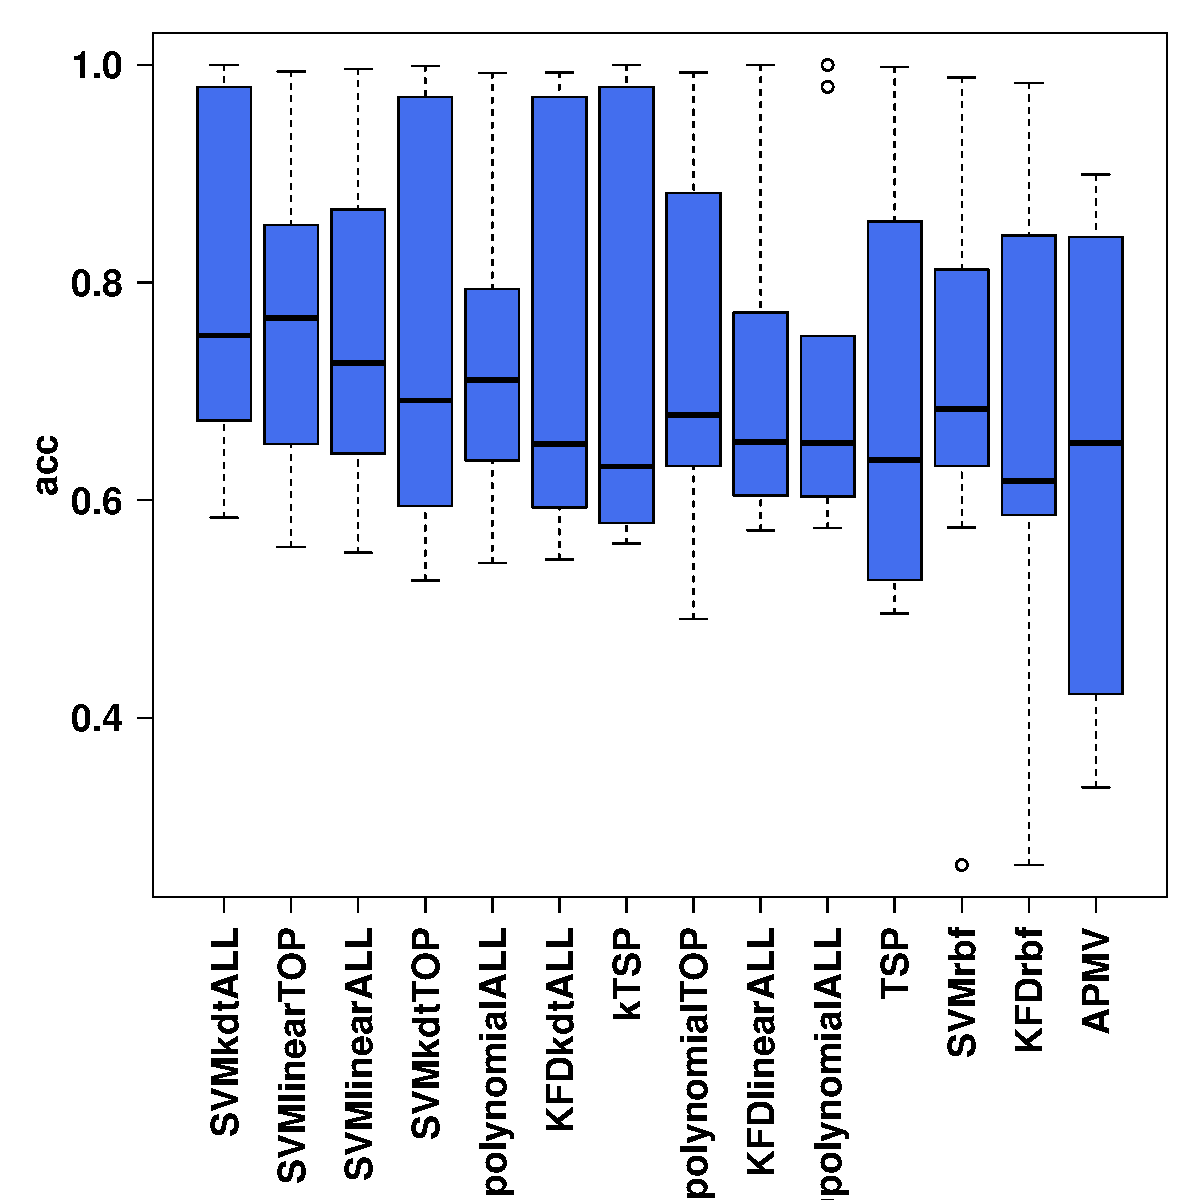
\includegraphics[width=0.6\textwidth]{ch-kendall/clasf_results/acc_plot}
\
\end{center}
\caption{Model performance comparison (ordered by decreasing average accuracy across datasets).}
\label{fig2:exprresult-acc}
\end{figure}




We further studied how the performance of different kernels depends on the choice of the $C$ parameter or the SVM (Figure \ref{fig2:exprresult-perfSVM}), and on the number of features used (Figure \ref{fig2:exprresult-perfFS}), on some representative datasets. We observe that compared to other kernels, an SVM with the Kendall kernel is relatively insensitive to hyper-parameter $C$ especially when $C$ is large, which corresponds to a hard-margin SVM. This may explain in part the success of SVMs in this setting, since the risk of choosing a bad $C$ during training is reduced. Regarding the number of features used in case of feature selection, we notice that it does not seem to be beneficial to perform feature selection in this problem, explaining why the Kendall kernel which uses all pairwise comparisons between features outperforms other kernels restricted to a subset of these pairs. In particular, the feature space of the Kendall and Mallows kernels is precisely the space of binary pairwise comparisons defined by \cite{Geman2004Classifying}, and the results show that instead of selecting a few features in this space as the Top Scoring Pairs (TSP)-family classifiers do \cite{Geman2004Classifying, Tan2005Simple, Xu2005Robust, Lin2009ordering}, one can simply work with \emph{all} pairs with the kernel trick.


\begin{figure}[!htbp]
\begin{center}

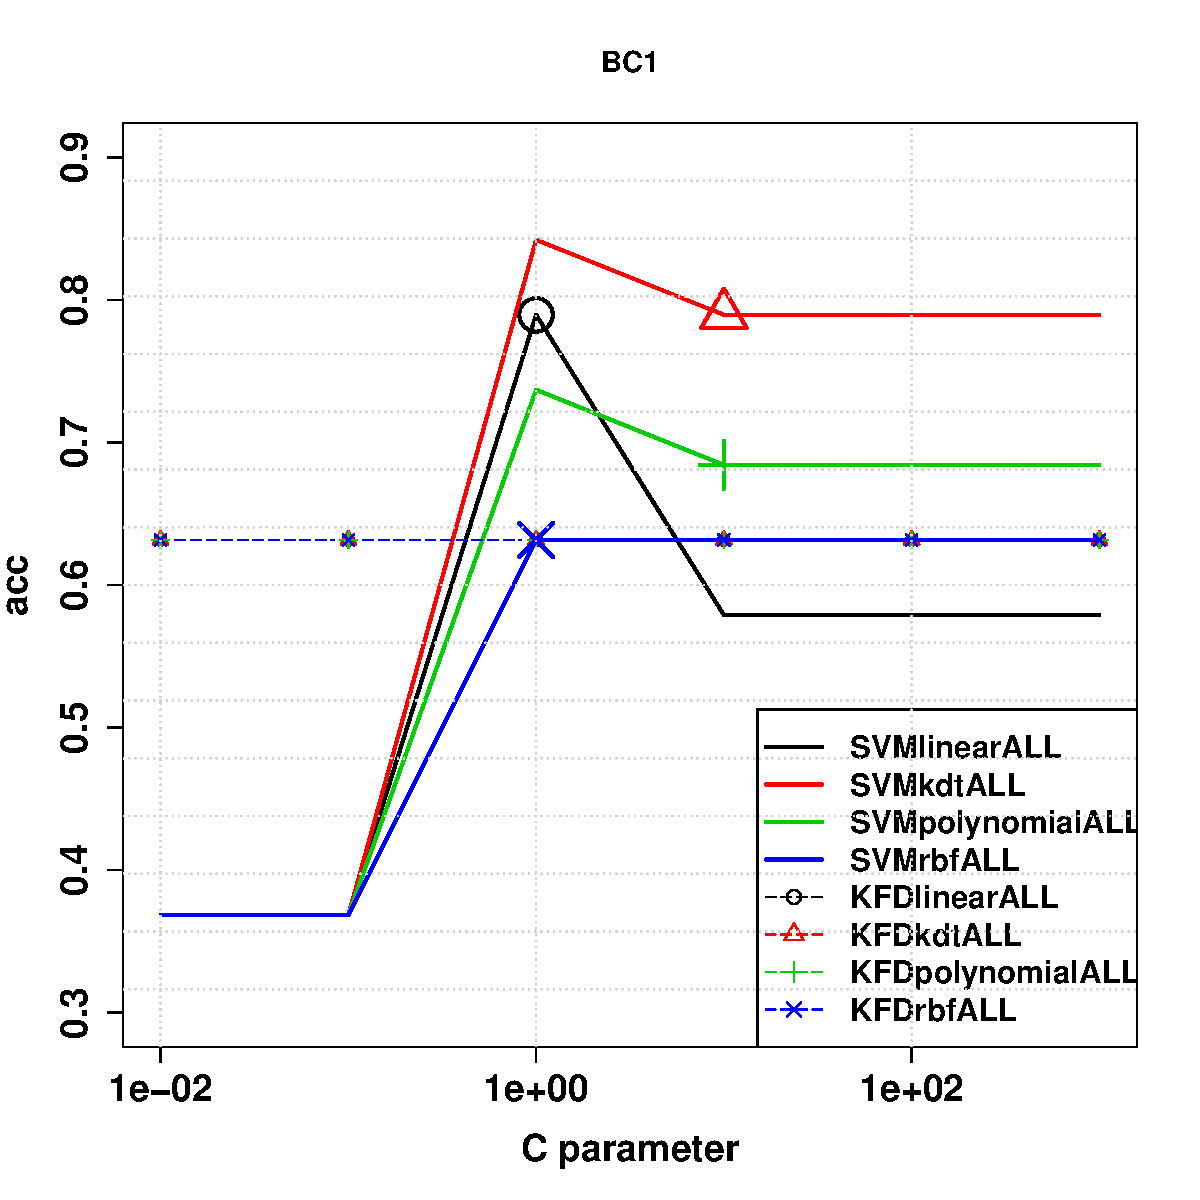
\includegraphics[width=0.6\textwidth]{ch-kendall/clasf_results/acc_perfSVM}

\end{center}
\caption{Sensitivity of kernel SVMs to $C$ parameter on the \emph{Breast Cancer 1} dataset. (Special marks on SVM lines denote the parameter returned by cross-validation.)}
\label{fig2:exprresult-perfSVM}
\end{figure}

\begin{figure}[!htbp]
\begin{center}

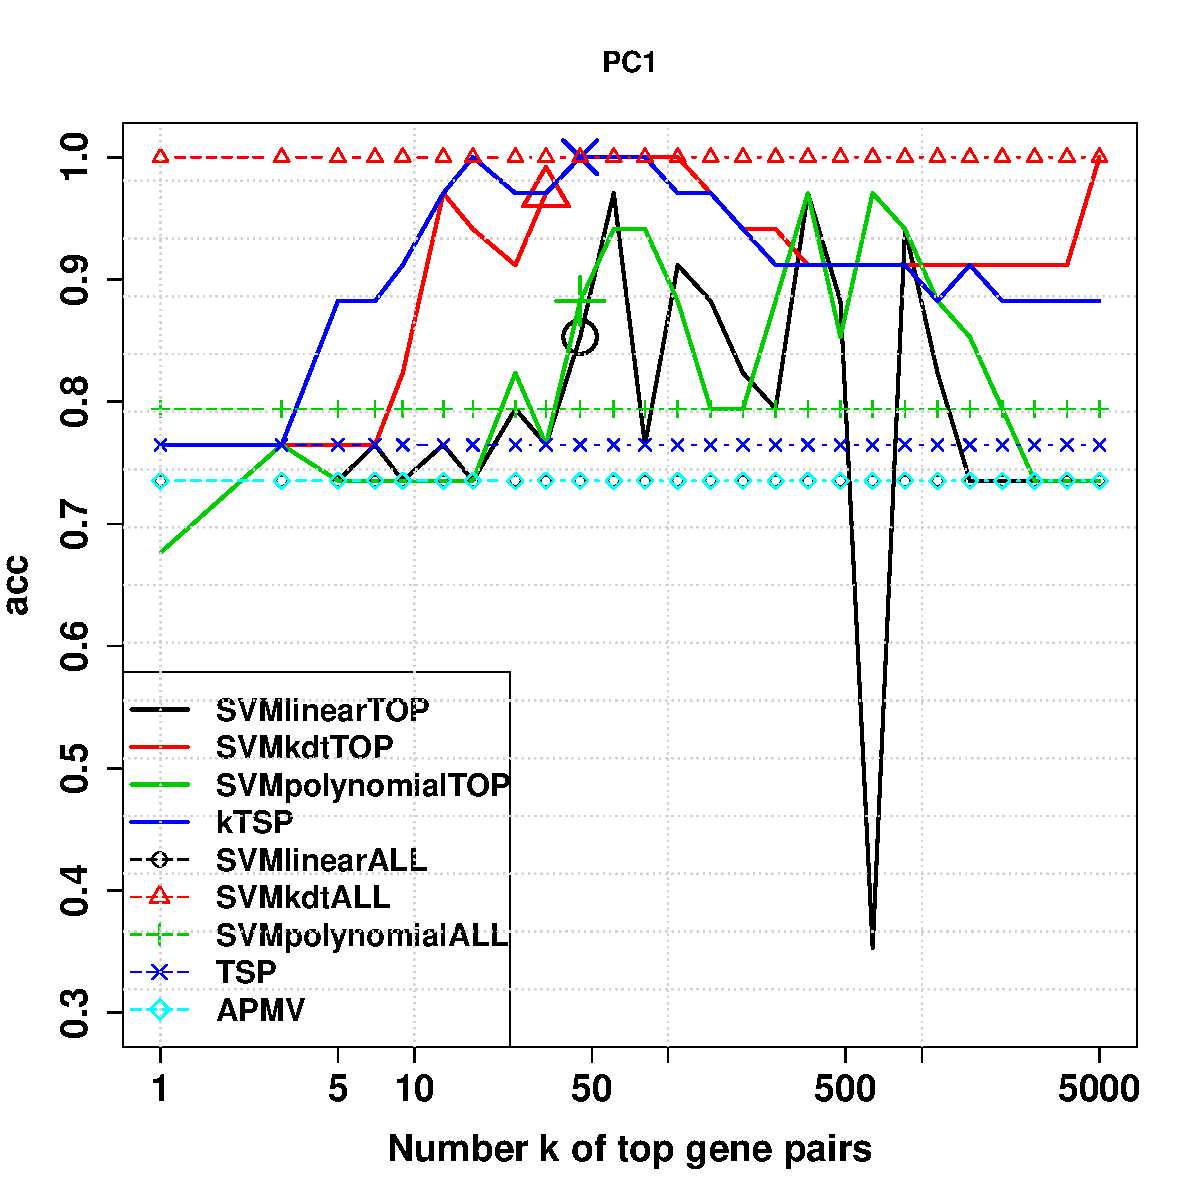
\includegraphics[width=0.6\textwidth]{ch-kendall/clasf_results/acc_perfFS}

\end{center}
\caption{Impact of TSP feature selection on the \emph{Prostate Cancer 1} dataset. (Special marks on SVM lines denote the parameter returned by cross-validation.)}
\label{fig2:exprresult-perfFS}
\end{figure}




Finally, as a proof of concept we empirically compare on one dataset the smooth alternative \eqref{eq2:G} and its Monte Carlo approximate \eqref{eq2:mc} with the original Kendall kernel. We studied how the performance varies with the amount of noise added to the samples (Figure \ref{fig2:exprapprox-stab}), and how the performance varies with the number of samples in the Monte Carlo scheme for a given amount of noise (Figure \ref{fig2:exprapprox-approxsingle}). It confirms that the smooth alternative \eqref{eq2:G} can improve the performance of the Kendall kernel, and that the amount of noise (window size) should be considered as a parameter of the kernel to be optimized. Although the $D^2$-sample Monte Carlo approximate kernel \eqref{eq2:mc} mainly serves as a fast estimate to the exact evaluation of \eqref{eq2:G}, it shows that the idea of jittered input with specific noise can also bring a tempting benefit for data analysis with Kendall kernel, even when $D$ is small. This also justifies the motivation of our proposed smooth alternative \eqref{eq2:G}. Last but not least, despite the fact that the convergence rate of $D^2$-sample Monte Carlo approximate to the exact kernel evaluation is guaranteed by Theorem \ref{thm2:approx}, experiments show that the convergence in practice is typically faster than the theoretical bound, and even faster in case that the window size $a$ is small. This is due to the fact that the convergence rate is also dependent of the observed data distribution in the input space, for which we have not made any specific assumption in our analysis.





\begin{figure}[!htbp]
\begin{center}
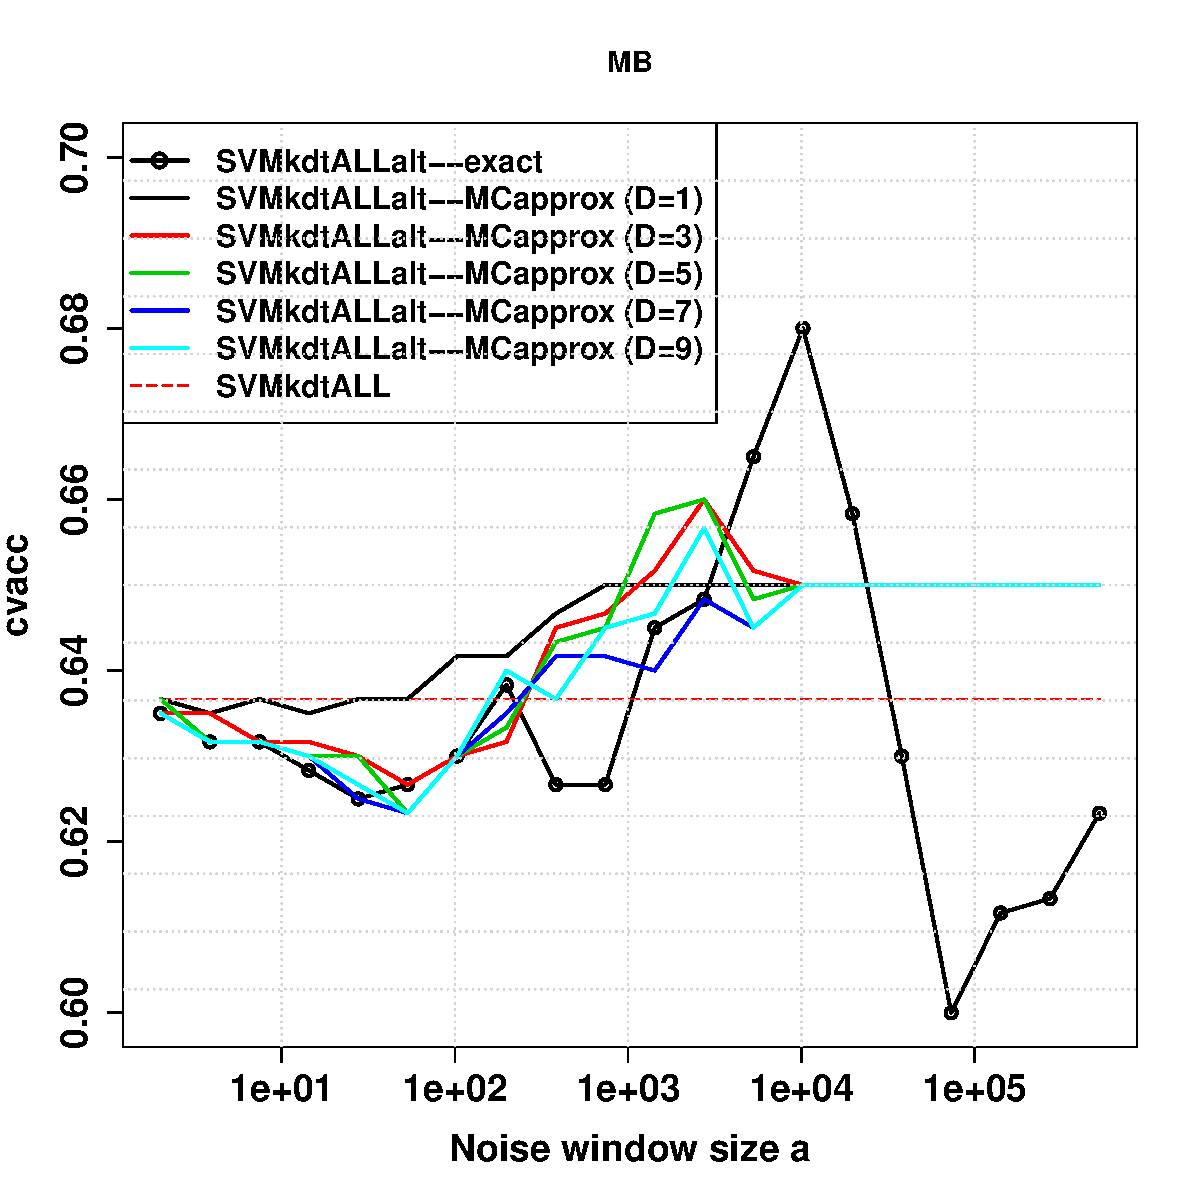
\includegraphics[width=0.6\textwidth]{ch-kendall/clasf_results/acc_StabApprox}
\end{center}
\caption{Empirical performance of smoothed alternative to Kendall kernel on the \emph{Medulloblastoma} dataset.}
\label{fig2:exprapprox-stab}
\end{figure}


\begin{figure}[!htbp]
\begin{center}
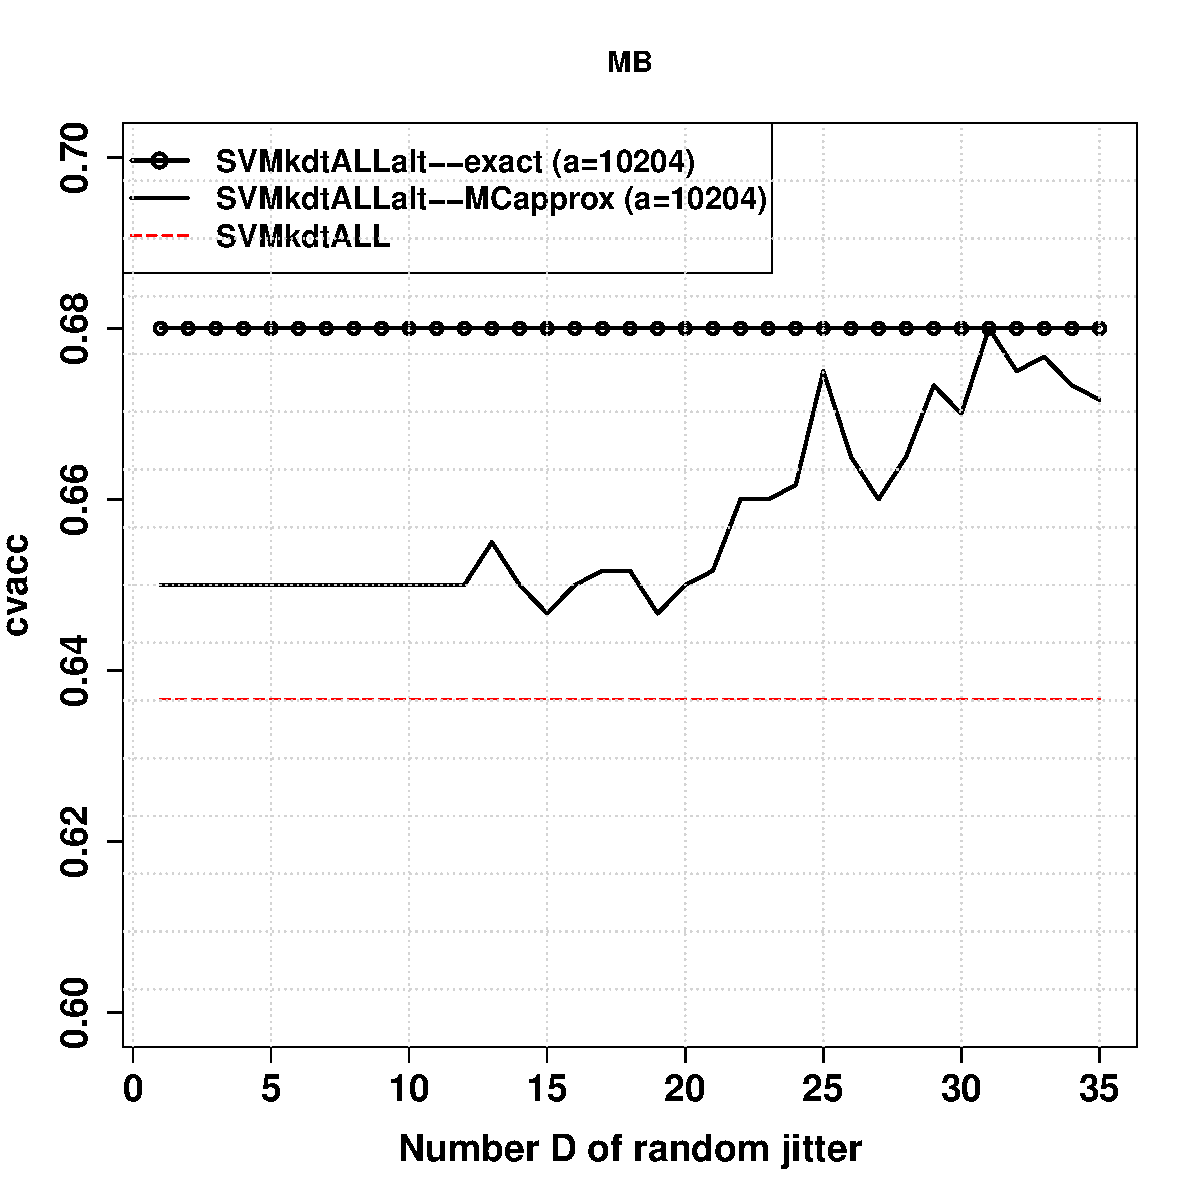
\includegraphics[width=0.6\textwidth]{ch-kendall/clasf_results/acc_approxSingleWindow}
\end{center}
\caption{Empirical convergence of Monte Carlo approximate at the fixed window size attaining maximum underlying accuracy from the left plot.}
\label{fig2:exprapprox-approxsingle}
\end{figure}




\section{Discussion}
\label{sec2:discussion}

Based on the observation that the popular Kendall tau correlation between total rankings is a positive definite kernel, we presented some extensions and applications pertaining to learning with the Kendall kernel and the related Mallows kernel. We showed that both kernels can be evaluated efficiently in $O(n \log n)$ time, and that the Kendall kernel can be extended to partial rankings containing $k$ items out of $n$ in $O(k \log k)$ time as well as to multivariate rankings. When permutations are obtained by sorting real-valued vectors, we proposed an extension of the Kendall kernel based on random perturbations of the input vector to increase its robustness to small variations, and discussed two possible algorithms to compute it. We further highlighted a connection between the fast Mallow kernel and the diffusion kernel of \cite{Kondor2010Ranking}. We also reported promising experimental results on clustering of heterogeneous rank data and classifying biomedical data demonstrating that for highly noisy data, the Kendall kernel is competitive or even outperforms other state-of-the-art kernels. 

We believe that computationally efficient kernels over the symmetric group pave the way to numerous applications beyond the ones we pursued in this chapter. In unsupervised data mining, kernel density estimation for example can be applied to modeling the distribution over a collection of rankings, and by the representer theorem the resulting distribution depends solely on the observed data points circumventing the exponentially large cardinality of the symmetric group, from which a consensus ranking that best represents the data is the one with the highest probability. As more complicated cases, there is much interest beyond finding a single consensus ranking typically in the context of political votes or social choices: groups of homogeneous sub-populations in data can be clustered by algorithms such as kernel $k$-means or spectral clustering \cite{Filippone2008survey}; dependencies or principle structural factors in data can be found by kernel canonical correlation analysis \cite{Lai2000Kernel} or kernel principle component analysis \cite{Schoelkopf1999Kernel}; outliers in a collection of rank data can be detected with one-class SVMs \cite{Schoelkopf1999Support,Tax2004Support}. In a more predictive setting, Support Vector Machines and kernel ridge regression are representative delegates for solving classification and regression problems amongst many other kernel algorithms \cite{Schoelkopf2002Learning}. Notably, the input/output kernels formalism allows us to predict rankings as well as learn from rankings where a wealth of algorithms such as multi-class SVMs or structural SVMs \cite{Crammer2002algorithmic,Tsochantaridis2005Large,Bakir2007Predicting} are ready to suit the problem at hand.

Deeper understanding of the Kendall and Mallows kernels calls for more theoretical work of the proposed kernels. In particular, a detailed analysis of the Fourier spectra of the Kendall and Mallows kernels is provided in \cite{Mania2016Universality}. Those authors also introduced a tractable family of normalized polynomial kernels of degree $p$ that interpolates between Kendall (degree one) and Mallows (infinite degree) kernels.

There are many interesting extensions of the current work. One direction would be to include high-order comparisons in measuring the similarity between permutations. Since the fast computation of the Kendall and Mallows kernels is balanced by the fact that they only rely on pairwise statistics between the ranks, computationally tractable extension to higher-order statistics, such as three-way comparisons, could potentially enhance the discriminative power of the proposed kernels. Another interesting direction would be to extend the proposed kernels to rankings on partially ordered set. In fact, the current work lies on the assumption that a (strict) total order can be associated with the (finite) set of items given to rank $\{x_1,\dots,x_n\}$, which is implicitly presumed when we label the items by the subscripts $\n$ and then define the Kendall and Mallows kernels by comparing all item pairs $(i,j)$ for $i<j$ (Section \ref{sec2:kernel}). However, there are cases when the item set is intrinsically associated with a (strict) partial order such that some item pairs are conceptually incomparable. In that case, we can collect all comparable item pairs into a set denoted by $E$ and define the kernels by comparing only those item pairs $(i,j)$ in $E$. Notably evaluating the extended kernels is still fast as we can simply replace the Merge Sort algorithm for total orders (Section \ref{sec2:kernel}) by a topological sort algorithm for partial orders \cite[Section 22.4]{Cormen2009Introduction}. We leave further investigations of this generalization to future work.

